\documentclass[11pt]{article}
\usepackage[T1]{fontenc}
\usepackage[utf8]{inputenc}
\usepackage{lmodern}
\usepackage[margin=1.08in]{geometry}
\usepackage{amsmath,amssymb,amsthm,mathtools,bm}
\usepackage{microtype}
\usepackage{enumitem,booktabs,array}
\usepackage{graphicx,xcolor,tikz}
\usetikzlibrary{arrows.meta,positioning,calc}
\usepackage[hyphens]{url}
\usepackage{hyperref}
\hypersetup{colorlinks=true,linkcolor=blue!45!black,citecolor=blue!45!black,
  urlcolor=blue!45!black,pdfauthor={OpenAI},
  pdftitle={Functional universality of critical SK autocorrelations}}
\numberwithin{equation}{section}
\newtheorem{theorem}{Theorem}[section]
\newtheorem{proposition}[theorem]{Proposition}
\newtheorem{lemma}[theorem]{Lemma}
\newtheorem{corollary}[theorem]{Corollary}
\theoremstyle{definition}
\newtheorem{definition}[theorem]{Definition}
\theoremstyle{remark}
\newtheorem{remark}[theorem]{Remark}
\newcommand{\E}{\mathbb E}
\renewcommand{\P}{\mathbb P}
\newcommand{\R}{\mathbb R}
\newcommand{\N}{\mathbb N}
\newcommand{\Z}{\mathbb Z}
\newcommand{\1}{\mathbf 1}
\newcommand{\cE}{\mathcal E}
\newcommand{\cA}{\mathcal A}
\newcommand{\cL}{\mathcal L}
\newcommand{\cH}{\mathcal H}
\DeclareMathOperator{\Tr}{Tr}
\DeclareMathOperator{\Cov}{Cov}
\DeclareMathOperator{\Var}{Var}
\DeclareMathOperator{\supp}{supp}
\DeclareMathOperator{\diag}{diag}
\DeclareMathOperator{\sech}{sech}
\DeclareMathOperator{\Id}{Id}
\DeclareMathOperator{\Ent}{Ent}
\DeclareMathOperator{\Law}{Law}
\newcommand{\articleid}[1]{\begingroup\urlstyle{same}\nolinkurl{#1}\endgroup}
\setlist[enumerate]{itemsep=3pt,topsep=5pt}
\setlist[itemize]{itemsep=3pt,topsep=5pt}
\setlength{\emergencystretch}{2em}
\allowdisplaybreaks[2]

\title{Functional universality of critical SK autocorrelations}
\author{OpenAI}
\date{October 5, 2026}
\begin{document}
\maketitle
\begin{abstract}
We prove that the stationary spin autocorrelation of the zero-field
Sherrington--Kirkpatrick model at inverse temperature $\beta=1$ has a common
functional scaling limit for Gaussian and Rademacher couplings. With
rate-one heat-bath clocks at every site, time is scaled by $n^{2/3}$ and the
mean spin autocorrelation is multiplied by $n^{1/3}$. The functions converge
in law uniformly on compact positive-time intervals. Their limiting law
is not a point mass: it retains sample-to-sample randomness, and its
functions decay to zero at large times.
\end{abstract}
\tableofcontents
\section{Introduction}\label{sec:introduction}

The equilibrium spin autocorrelation measures how much a system remembers
its initial configuration after averaging over its stationary dynamics.
At the critical temperature of the Sherrington--Kirkpatrick model, this
memory lives on a time scale that diverges with the number of spins.
We determine its limiting random function and prove that Gaussian and
Rademacher interactions give the same law on the stated clock.

\subsection{Model and result}
Let $D$ be either the standard Gaussian distribution or the uniform
distribution on $\{-1,1\}$. For $n\ge2$, let $(J_{ij})_{i<j}$ be independent
with law $D$, put $J_{ji}=J_{ij}$ and $J_{ii}=0$, and define
\begin{equation}\label{eq:intro-gibbs}
 \pi_{n,J}(\sigma)=\frac1{Z_{n,J}}
 \exp\left(\frac1{\sqrt n}\sum_{i<j}J_{ij}\sigma_i\sigma_j\right),
 \qquad \sigma\in\{-1,1\}^n.
\end{equation}
This is the zero-field model at inverse temperature one. Each site has an
independent rate-one clock. When the clock at site $i$ rings, its spin is
resampled from its conditional law under $\pi_{n,J}$:
\[
 \P\{\sigma_i\gets a\mid\sigma_{-i}\}
 =\frac{\exp(a h_i(\sigma))}{2\cosh h_i(\sigma)},
 \qquad h_i(\sigma)=\frac1{\sqrt n}\sum_{j\ne i}J_{ij}\sigma_j.
\]
One unit of this clock contains $n$ site updates on average.
Write $P_t^J$ for this reversible semigroup. Its stationary spin
autocorrelation and its critical rescaling are
\begin{align}
 C_{n,J}(t)&=\frac1n\sum_{i=1}^n
    \langle\sigma_i,P_t^J\sigma_i\rangle_{\pi_{n,J}},
       \label{eq:intro-correlation}\\
 A_{n,J}(s)&=n^{1/3}C_{n,J}(s n^{2/3}),\qquad s>0.
       \label{eq:intro-rescaling}
\end{align}
Thermal fluctuations and the randomness of the dynamics have already been
averaged in these quantities. Their only remaining randomness is the
interaction matrix.

Let $C_{\mathrm{loc}}((0,\infty))$ denote the continuous real functions,
with uniform convergence on every compact subinterval of $(0,\infty)$.

\begin{theorem}[Functional universality]\label{thm:main}
There is a Borel probability law $Q_{\mathrm{crit}}$ on
$C_{\mathrm{loc}}((0,\infty))$ such that, for each of the two choices of $D$,
\[
 \Law_D(A_{n,J})\Longrightarrow Q_{\mathrm{crit}}
 \qquad(n\to\infty).
\]
The law $Q_{\mathrm{crit}}$ is not a point mass. It assigns probability one
to nonzero, nonnegative, nonincreasing functions $f$ satisfying
$\lim_{s\to\infty}f(s)=0$. The Gaussian and Rademacher models use exactly
the normalization in \eqref{eq:intro-rescaling}.
\end{theorem}

The restriction to positive times is necessary: $A_{n,J}(0)=n^{1/3}$.
At every fixed positive time, the limiting value has unbounded support,
as proved in Proposition~\ref{prop:functional-randomness}.
The limiting law is described explicitly in Section~\ref{sec:edge-law}.
It is the law of a sum of coordinate autocorrelations for a reversible semigroup in
countably many edge coordinates.
The equilibrium measure of those coordinates is Gaussian conditioned on a
renormalized quadratic constraint; its parameters are the random GOE edge
points. A single positive deterministic coefficient accounts for the
relaxation of microscopic spin gradients. Section~\ref{sec:microscopic}
characterizes that coefficient by a determinate moment problem.

\subsection{History and relation to earlier work}
Sherrington and Kirkpatrick introduced their infinite-range spin-glass
model in 1975~\cite{SK1975}. Dynamical mean-field theory subsequently studied
relaxation through correlation and response, notably in the soft-spin
framework of Sompolinsky and Zippelius~\cite{SompolinskyZippelius1982}.
For critical Ising heat-bath dynamics, Billoire and
Campbell~\cite[Equation~(7)]{BilloireCampbell2011} tested numerically the
finite-size scaling form
\[
 q_c(n,t)\sim n^{-1/3}F(t/n^{2/3}),
\]
with time measured in updates per spin. This is the direct numerical
precedent for \eqref{eq:intro-rescaling}. A disorder-averaged scaling curve
does not determine whether individual sample curves concentrate; our result
identifies their limiting probability law.

Spherical models made the role of the spectral edge especially clear.
Kosterlitz, Thouless, and Jones~\cite{KosterlitzThoulessJones1976} identified
the edge mechanism in the spherical spin-glass transition.
Cugliandolo and Dean~\cite{CugliandoloDean1995} analyzed Langevin relaxation
and aging, and Ben Arous, Dembo, and Guionnet~\cite{BenArousDemboGuionnet2001}
proved limiting dynamics and aging results for a soft spherical constraint.
At finite size, Fyodorov, Perret, and Schehr~\cite{FyodorovPerretSchehr2015}
related non-self-averaging on the $n^{2/3}$ time scale to edge fluctuations
in zero-temperature spherical dynamics. These are spectral and dynamical
predecessors, with different temperatures, initial conditions, and spin
spaces from stationary critical Ising heat-bath dynamics.

The equilibrium comparison used here has its own history.
Comets~\cite{Comets1996} related Ising and spherical partition functions by
averaging over the eigenframe. Baik and Lee~\cite{BaikLee2016} studied
spherical free-energy fluctuations on the two sides of the transition,
and Landon~\cite{Landon2022} analyzed critical free-energy fluctuations and
the edge-scale saddle. Du and Huang~\cite{DuHuang2026FreeEnergy} obtained
a quantitative critical Ising--spherical partition comparison; their
quenched overlap theorem~\cite{DuHuang2026Overlap} describes the random
critical overlap law using Gaussian coordinates conditioned on a
centered square sum. The conditioned measure used below follows this framework.
The additional work here identifies the closed dynamical form, its
microscopic coefficient, and the functional limit across two coupling laws.

Rigorous high-temperature mixing developed through spectral functional
inequalities and localization. Relevant steps include
Bauerschmidt and Bodineau~\cite{BauerschmidtBodineau2019},
Eldan, Koehler, and Zeitouni~\cite{EldanKoehlerZeitouni2022}, and
Anari, Koehler, and Vuong~\cite{AnariKoehlerVuong2024}.
For fixed inverse temperature $\beta<1/2$, Wang~\cite{Wang2026} obtains
$O_\beta(n\log(n/\epsilon))$ random-site heat-bath mixing, uniformly in
external fields, with probability tending to one over the disorder.
At zero field, Boban, Li, and Oveis
Gharan~\cite{BobanLiOveisGharan2026} obtain a spectral gap bounded below by
a positive constant for rate-one-per-site dynamics, and polynomial mixing
for $\beta<1/2+\epsilon_0$, with a universal
$\epsilon_0>0$, again with high disorder probability.
Such fixed-subcritical estimates do not identify dynamics
at the endpoint $\beta=1$.

Two companion manuscripts supply the Gaussian estimates used below.
The critical slowing-down manuscript~\cite[Theorems~1.1 and~1.2]{CS} identifies the $n^{2/3}$
scale of covariance and linear relaxation, and gives an obstruction to
mixing from most realized equilibrium starts at smaller times. The critical
mixing manuscript~\cite[Theorem~1.1]{CM} obtains the matching mixing exponent and
functional inequalities. Its comparison of spectral caps with spherical
measures provides the starting estimates for our proof. An exponent statement
alone does not identify the dynamics at a fixed multiple of $n^{2/3}$;
we need quantitative improvements and an identification of the limiting
energy. We state the companion inputs with their precise ranges in
Section~\ref{sec:edge-law} and prove those additional steps here.

Finally, the comparison of coupling laws belongs to the Lindeberg approach
to universality~\cite{Chatterjee2006}. Carmona and Hu~\cite{CarmonaHu2006}
proved universality of the SK limiting free energy. The observable here
depends on the Gibbs law and the generator simultaneously. Its critical
derivative bounds require the quadratic-feature comparison described next.

\subsection{The proof and its main ingredients}
We first work with Gaussian couplings. Adjoining an independent Gaussian
diagonal does not affect the Gibbs law and makes the interaction matrix a
GOE matrix $W=U\Lambda U^{\mathsf T}$. The spectral coordinates
$x=n^{-1/3}U^{\mathsf T}\sigma$ isolate the fluctuations near the upper edge.
Their limiting equilibrium law is a conditioned measure $\Pi$, rather than
a product of independent Gaussian coordinates. This constraint remains
visible in the domain of the limiting gradient form.

There are two separate reasons why equilibrium convergence does not already
give the answer. First, a function of the edge coordinates can lower its
Dirichlet energy by adding a small microscopic correction. Second, convergence
of finitely many edge coordinates gives no bound on the sum over all
coordinates in \eqref{eq:intro-correlation}. The proof treats these issues
before comparing the two coupling distributions.

The starting observation is the resolvent trace. If $H$ is minus the
heat-bath generator, then for $z>0$ set
\[
 B_n(z)=\sum_{a=1}^n
   \langle x_a,(z+n^{2/3}H)^{-1}x_a\rangle.
\]
This quantity is independent of the choice of orthogonal coordinates. It
is the Stieltjes transform of the same spectral measure whose Laplace
transform is $A_{n,J}$. We establish convergence of these traces and then
recover convergence of the functions on every compact positive time interval.

The observations used below have a concrete spectral meaning. At scale
$p>0$, remove from $W$ the matrix
\[
 B_p=U\diag\bigl((\lambda_a-(2-p^2))_+\bigr)U^{\mathsf T},
 \qquad h_p=B_p\sigma+\mathsf N(0,B_p).
\]
Conditioning on $h_p$ replaces the interaction by $W-B_p$, whose eigenvalues
are capped at $2-p^2$, and adds the external field $h_p$. Decreasing $p$
retains fewer observed directions near the spectral edge.

The Gaussian argument has four stages.
\begin{enumerate}
\item Spectral observations smooth functions on the cube. We compare their
posterior means with a spherical model and control the score of the
comparison density. Sections~\ref{sec:observations} and~\ref{sec:variance}
sharpen the cap estimates to a conditional variance bound of order $p^{-2}$
at cap scale $p$, without a power loss. The gain comes from averaging the
curvature error before compressing it onto a smaller random spectral subspace.
\item In Section~\ref{sec:gradient}, slopes of these smoothings converge to
weak gradients for $\Pi$. We prove that their domain equals the closure of
smooth cylinder functions. This identifies the closed energy form on the
conditioned equilibrium measure.
\item Section~\ref{sec:microscopic} identifies the energy remaining after
microscopic correction. Fixed-order contractions specify a deterministic
positive measure $\omega$ on $[0,\infty)$. Polynomial approximation isolates
its atom $c_*=\omega(\{0\})$, producing matching lower bounds and recovery
sequences for the limiting form $c_*\int|\nabla F|^2\,d\Pi$.
\item Section~\ref{sec:trace} bounds the tail of the resolvent trace by vector
integration by parts. The summable decay of the resulting coefficients makes
finite-coordinate convergence sufficient for the whole observable.
\end{enumerate}

For Rademacher couplings we compare basis-independent traces directly.
The Lindeberg argument in Section~\ref{sec:comparison} first transfers a
trace built from quadratic spin features. Its vanishing controls the
fourth-order remainders for the spin trace. This order of comparison is what
allows Gaussian and sign couplings, whose fourth moments differ, to have
the same limit. Finally, Section~\ref{sec:functional} proves the functional
convergence, decay, and surviving disorder randomness. Appendix~\ref{sec:support}
explains why almost-sure decay is compatible with nondecaying functions in
the closed topological support.

\section{The conditioned edge measure and the Gaussian inputs}
\label{sec:edge-law}

The limiting state space is determined by the upper spectral edge of the
interaction matrix.  The spherical model makes this state space explicit:
after diagonalization, its only remaining interaction is a constraint on the
sum of the squared coordinates.  We construct the resulting probability measure on infinitely many coordinates, following the equilibrium
edge-conditioning description of Du--Huang \cite[Section~2]{DuHuang2026Overlap}.  We then explain the change of disorder law that transfers spherical
calculations to the cube, and record the cap estimates used in the dynamical
argument.

\subsection{The heat-bath form and the edge coordinates}

Write $\mu=\pi_{n,J}$ and put $T=n^{2/3}$.  For a function on the cube, let
\[
 D_i f(X)=\frac{f(X^{i,+})-f(X^{i,-})}{2},\qquad
 t_i(X)=\tanh h_i(X),\qquad w_i(X)=1-t_i(X)^2,
\]
where $X^{i,\pm}$ is obtained by setting the $i$th spin to $\pm1$ and
$h_i(X)=n^{-1/2}\sum_{j\ne i}J_{ij}X_j$.  The nonnegative heat-bath
operator and its Dirichlet form are
\begin{equation}\label{eq:edge-heatbath-form}
 H=\sum_{i=1}^n(X_i-t_i)D_i,
 \qquad
 \cE(f,g)=\mu\!\left[\sum_{i=1}^n w_iD_ifD_ig\right],
 \qquad \cE(f)=\cE(f,f).
\end{equation}
Thus $P_t^J=e^{-tH}$.  Forms and inner products of vector-valued functions
include summation over the vector index.  In particular, the clock
normalization in \eqref{eq:edge-heatbath-form} is rate one at each site.

Until Section~\ref{sec:comparison}, the couplings are Gaussian.  Let $W$ have
off-diagonal entries $J_{ij}/\sqrt n$, and add independent diagonal entries
with law $N(0,2/n)$.  The extra energy is constant on the cube, so it changes
neither $\mu$ nor $H$.  The completed matrix is GOE.  Diagonalize it as
\[
 W=U\Lambda U^{\mathsf T},\qquad
 \lambda_1\ge\cdots\ge\lambda_n,
 \qquad d_a=2-\lambda_a,\qquad g_{a,n}=n^{2/3}d_a.
\]
After independent choices of eigenvector signs, $U$ is Haar orthogonal
conditionally on $\Lambda$.  Its columns are denoted by $v_a$.  Set
\[
 Y_a=v_a^{\mathsf T}X,\qquad x_a=n^{-1/3}Y_a,
 \qquad
 B_n(z)=\sum_{a=1}^n\langle x_a,(z+TH)^{-1}x_a\rangle_\mu,
 \quad z>0.
\]
The trace $B_n(z)$ is independent of the chosen orthonormal basis and is
the Laplace transform of the rescaled autocorrelation:
\[
 B_n(z)=\int_0^\infty e^{-zs}A_{n,J}(s)\,ds.
\]
We use $x_a$ also for the coordinate functions of the limiting measure.

Let $\rho_{\rm sc}$ be the semicircle probability measure
\[
 d\rho_{\rm sc}(\lambda)=\frac1{2\pi}
 \sqrt{4-\lambda^2}\,\1_{[-2,2]}(\lambda)\,d\lambda.
\]
The GOE edge convergence theorem gives the joint convergence of each fixed
number of $g_{a,n}$ to a simple, increasing point process
$g=(g_1,g_2,\ldots)$; see \cite{RamirezRiderVirag2011}.  This definition fixes the sign and
scale of the edge process throughout the paper.

\begin{lemma}[Spectral bounds]\label{lem:edge-spectral}
The GOE eigenvalues have the following additional properties.
\begin{enumerate}
\item $\max_a|\lambda_a|\le3$ with probability tending to one.
\item There are tight random bounds $K_n\ge0$ and $C_n>0$ such that
$g_{a,n}\ge C_n^{-1}a^{2/3}$ for every $a>K_n$.
\item For every $\epsilon>0$,
\begin{equation}\label{eq:edge-trace-double-limit}
 \lim_{L\to\infty}\limsup_{n\to\infty}
 \mathbb P\!\left(
 g_{1,n}+L\le0\ \text{or}\
 \left|n^{1/3}-\sum_{a=1}^n\frac1{g_{a,n}+L}-\sqrt L\right|
       >\epsilon\right)=0.
\end{equation}
\end{enumerate}
In the event appearing in the last formula, the sum is evaluated only when
$g_{1,n}+L>0$.
\end{lemma}

\begin{proof}
We use the eigenvalue-only spectral estimate of \cite[Proposition~3.1]{CS}.  For every
deterministic sequence $L_n\to\infty$ with $L_n\le\log n$, that proposition
controls both resolvent traces for
$s\in[L_nn^{-2/3},5]$, with positive denominators.  At
$s=L_nn^{-2/3}$, multiplying its first-trace error by $n^{1/3}$ gives
\[
 O\!\left(L_n^{-1}+L_n^{-1/8}
       +L_n^{-1/4}\sqrt{\log(2+L_n)}\right)=o(1).
\]
The semicircle resolvent equals
$(2+s-\sqrt{s(4+s)})/2$, whose expansion supplies the main term
$\sqrt{L_n}$ and an additional error $O(L_nn^{-1/3})=o(1)$.

The second-trace estimate yields, for the same interval of $u$,
\[
 \#\{a:d_a\le u\}
 \le 4u^2\sum_a(d_a+u)^{-2}
 \le Cnu^{3/2}.
\]
Indeed $0<d_a+u\le2u$ for every counted eigenvalue.  It follows that
$g_{a,n}\ge c a^{2/3}$ once $a>CL_n^{3/2}$.  The uniform norm bound is
part of the same proposition.

These conclusions hold for every arbitrarily slowly divergent $L_n$.
If \eqref{eq:edge-trace-double-limit} failed, one could select
$L_j\to\infty$ and $n_j\to\infty$, with $\log n_j\ge L_j$, along which
the failure probability stayed positive, and embed the values
$L_{n_j}=L_j$ in a sufficiently slow divergent sequence.  This contradicts
the preceding estimate.  The identical criterion, applied to the least
index after which the counting consequence holds, makes that index tight.
This proves the second assertion as well.
\end{proof}

\begin{remark}[Convergence on sets of large disorder probability]
\label{rem:edge-tight-convergence}
We will use constants that are bounded on disorder events of probability
arbitrarily close to one.  A bound of this kind is called a tight bound.
For subsequential arguments, include these bounds, the eigenvalues, and the
countably many relevant error quantities in the joint law before taking a
Skorokhod representation.  On the represented space, finite bounds and
coordinate convergence can then be used deterministically.  The conditional
laws of the remaining finite-dimensional variables lift this representation
to the original finite problems.  A further diagonal extraction handles
quantities that vanish in an iterated limit such as
\eqref{eq:edge-trace-double-limit}.  The representation itself makes no assertion of convergence for the
original sequence: one must identify every subsequential limit.  Once this
identification is made, the subsequence criterion gives the asserted joint
convergence in distribution.  In particular, if every subsequence of an
intrinsic error quantity has a further represented subsequence tending to
zero, that quantity tends to zero in probability on the original disorder
space.  No uniform integrability on exceptional disorders is required.

A separate uniformity convention is essential for variational arguments.
When an estimate is applied to a disorder-dependent test, its quenched
inequality is understood to hold on one event for every test in the stated
class, with the displayed bounds on its norm, energy, and polynomial growth.
One way to obtain such an event, used below, is to bound the error for every
test by its stated norms times a common nonnegative random error $R_n$.
Convergence $R_n\to0$ then permits arbitrary measurable choices of the test.
Convergence on a countable core alone is not used to infer this uniformity.
\end{remark}

\subsection{Conditioning the infinite Gaussian family}

Choose an admissible parameter $b$ with $b+g_1>0$, and write
$l_a=(g_a+b)^{-1}$.  A convenient measurable choice is
$b=1+(-g_1)_+$; use the corresponding $b_n=1+(-g_{1,n})_+$ in finite
dimension.  By Lemma~\ref{lem:edge-spectral},
\[
 l_{a,n}=(g_{a,n}+b_n)^{-1}\longrightarrow l_a,
 \qquad
 \lim_{m\to\infty}\sup_n\sum_{a>m}l_{a,n}^2=0
\]
on the represented sets just described, after discarding finitely many
initial $n$.  In particular $\sum_a l_a^2<\infty$.

For independent $Z_a\sim N(0,l_a)$, the centered series
$S=\sum_a(Z_a^2-l_a)$ converges almost surely and in $L^2$.  Define
\begin{equation}\label{eq:source-1}
 D(b)=\lim_{L\to\infty}\left\{
 \sqrt L-\sum_{a\ge1}\left(\frac1{g_a+b}-\frac1{g_a+L}\right)\right\}.
\end{equation}
Here $L$ is restricted to values with $L+g_1>0$.  The limit is in probability
with respect to $g$; a deterministic subsequence gives an almost sure
version.  The next proposition both justifies the limit and gives a
pointwise meaning to conditioning on $S=D(b)$.

\begin{proposition}[The conditioned edge measure]
\label{prop:edge-conditioned-law}
Formula~\eqref{eq:source-1} defines a finite random variable, and
\[
 D_n(b_n):=n^{1/3}-\sum_{a=1}^n l_{a,n}
       \ \Longrightarrow\ D(b)
\]
jointly with the edge coordinates.  Almost surely $\sum_a l_a=\infty$.
The law of $(Z_a)_{a\ge1}$ conditioned on $S=D(b)$ has a version
$\Pi=\Pi_g$ characterized by continuous conditional densities.  It is
independent of the admissible choice of $b$.

Let $\mu^{\rm sp}$ denote normalized surface measure on the sphere of
radius $\sqrt n$, tilted by $\exp(X^{\mathsf T}WX/2)$.  The fixed-coordinate marginals of $n^{-1/3}U^{\mathsf T}X$ under
$\mu^{\rm sp}$ converge jointly in distribution with the eigenvalues to
the random marginals of $\Pi$.  On the spectral representations of
Remark~\ref{rem:edge-tight-convergence}, this is ordinary weak convergence
of measures, including convergence of every fixed polynomial moment.  On the sets in Remark~\ref{rem:edge-tight-convergence},
for every fixed $0\le j<\infty$ one has
\begin{equation}\label{eq:edge-coordinate-moments}
 \int |x_a|^j\,d\Pi\le C_j l_a^{j/2},
 \qquad
 \mu^{\rm sp}|x_a|^j\le C_j l_{a,n}^{j/2},
\end{equation}
uniformly in the retained coordinate $a$.

For any sufficiently large fixed $m$, the tail $(x_a)_{a>m}$ under
$\Pi$ has a density relative to $\bigotimes_{a>m}N(0,l_a)$.  Conditional
on this tail, the first $m$ coordinates lie on the sphere of squared radius
\begin{equation}\label{eq:edge-polar-radius}
 D(b)+\sum_{a\le m}l_a-\sum_{a>m}(x_a^2-l_a),
\end{equation}
with the Gaussian angular density on that sphere.  In particular,
$\sum_a(x_a^2-l_a)=D(b)$ holds $\Pi$-almost surely.
\end{proposition}

\begin{proof}
For fixed admissible $L$, the identity
\[
 D_n(b_n)=n^{1/3}-\sum_a\frac1{g_{a,n}+L}
 -\sum_a\left(\frac1{g_{a,n}+b_n}-\frac1{g_{a,n}+L}\right)
\]
separates the divergent trace from an absolutely convergent difference.
The tail of the second sum is bounded by a constant times
$|L-b_n|\sum_{a>m}a^{-4/3}$ on each set of bounded spectral data, so that
sum passes to the limit.  Lemma~\ref{lem:edge-spectral} then shows that the
expressions in braces in \eqref{eq:source-1} are Cauchy in probability,
and that $D_n(b_n)$ has the asserted joint limit.  If $\sum_a l_a$ were
finite, those expressions would tend to $+\infty$ as $L\to\infty$;
this contradicts the finite limit.  Changing $b$ changes $D(b)$ by the
corresponding absolutely convergent resolvent difference.

We give the density argument explicitly.  Let $q$ be the density of $S$,
and let $q_m$ be the density of $\sum_{a>m}(Z_a^2-l_a)$.
After any fixed coordinates are omitted, a sufficiently large fixed group
of remaining coordinates supplies an integrable bound for the characteristic
function: the modulus of the factor for coordinate $a$ is
$(1+4t^2l_a^2)^{-1/4}$.  Fourier inversion therefore gives continuous,
bounded densities.  The same bound applies to the finite sums and proves
uniform convergence of their densities when the variances converge and
their squared tails vanish.

The centered sum after any finite deletion has support all of $\R$.
Its unbounded right support comes from one square.  To reach an arbitrarily
negative interval, make a sufficiently long finite block of squares small,
using $\sum l_a=\infty$, and keep the remaining centered sum in a bounded
interval of positive probability.  Convolution with a finite block whose
square-sum density is positive in the interior of its support now gives
$q(s)>0$ and $q_m(s)>0$ for every $s\in\R$.  Thus the first $m$
coordinates of the required conditional law have density
\begin{equation}\label{eq:edge-cylinder-density}
 \frac{q_m\!\left(D(b)-\sum_{a\le m}(x_a^2-l_a)\right)}{q(D(b))}
 \prod_{a\le m}\frac{e^{-x_a^2/(2l_a)}}{\sqrt{2\pi l_a}}.
\end{equation}
Convolution shows that these densities are consistent.  They depend
measurably on the spectral data, so their extension is a random probability
measure $\Pi_g$.

For completeness, they admit a disintegration on the constraint itself.
Let $q^{\rm head}_m$ be the density of
$\sum_{a\le m}(Z_a^2-l_a)$.  Give the tail product Gaussian law the
weight
\[
 \frac{q^{\rm head}_m\!\left(D(b)-\sum_{a>m}(x_a^2-l_a)\right)}{q(D(b))}.
\]
Given the tail, use polar disintegration of the first $m$ Gaussian
coordinates at the radius \eqref{eq:edge-polar-radius}.  This produces
\eqref{eq:edge-cylinder-density}, has an absolutely continuous tail law,
and enforces the constraint almost surely.

In finite dimension, conditioning independent normals of variances
$l_{a,n}$ on $\sum_a x_a^2=n^{1/3}$ gives exactly the spherical Gibbs
measure in the stated coordinates: the term involving $b_n$ in the Gaussian
exponent is constant on that sphere.  The density convergence above and
$q(D(b))>0$ imply convergence of each cylinder marginal.  Their densities
are bounded by a constant times the corresponding product Gaussian
density.  To retain an arbitrary single coordinate uniformly, choose the
integrable Fourier bound from a fixed group of leading coordinates other
than that coordinate.  This proves \eqref{eq:edge-coordinate-moments}
and uniform integrability of all fixed polynomial moments.

The argument applies to every admissible $b$ on sets where its distance
from the pole is bounded below and its magnitude is bounded above; these
sets exhaust the admissible choices.  The finite conditioned spherical law
is independent of $b_n$, so its limiting cylinder marginals are also
independent of $b$.  The conclusion holds simultaneously for all
admissible $b$.  First take a common probability-one event for rational
parameters.  On every compact admissible interval, the resolvent-difference
series converges uniformly, so $D(b)$ is continuous.  The squared variance
tails and the Fourier majorants above are also uniform on that interval.
Thus the conditional cylinder densities in
\eqref{eq:edge-cylinder-density}, and their integrals against bounded
continuous cylinder tests, depend continuously on $b$.  Equality for
rational parameters therefore extends to the whole interval.
\end{proof}

\begin{lemma}[The bulk spectral weight]\label{lem:edge-bulk-weight}
For a spherical Gibbs spin, the random probability measure
\[
 \frac1n\sum_a Y_a^2\delta_{\lambda_a}
\]
converges in probability, conditionally on the spectral data as above, to
$(2-\lambda)^{-1}d\rho_{\rm sc}(\lambda)$.
\end{lemma}

\begin{proof}
First test against a bounded continuous function supported away from $2$.
Before conditioning, the Gaussian variance of its integral is $O(n^{-1})$,
and its mean converges to the stated integral by the semicircle law.
Integrate out a fixed number of leading Gaussian coordinates when imposing
the norm constraint.  Their square-sum density gives a bounded density
ratio, so the concentration persists after conditioning.  Each of those
leading coordinates has mass $n^{-1/3}x_a^2=o(1)$ in probability by
\eqref{eq:edge-coordinate-moments}.  Finally both the finite measure and
its proposed limit have mass one, since
$\int(2-\lambda)^{-1}d\rho_{\rm sc}(\lambda)=1$.  This extends convergence
across the edge.  The same argument permits bounded tests with cuts at
continuity points in the bulk.
\end{proof}

\subsection{The limiting autocorrelation and its time constant}

For a smooth compactly supported cylinder function $F$ on $\R^{\N}$,
consider the quadratic form
\[
 \cE_\Pi(F)=\int\sum_a|\partial_aF|^2\,d\Pi.
\]
Proposition~\ref{prop:gradient-domain} will prove that this form is
closable and identify its domain.  Denote the nonnegative operator associated
to its closure by $H_\Pi$.  The law in Theorem~\ref{thm:main} is specified by
\begin{equation}\label{eq:source-2}
 \cA(s)=\sum_{a\ge1}
 \langle x_a,e^{-s c_*H_\Pi}x_a\rangle_\Pi,
 \qquad s>0,
\end{equation}
where $c_*>0$ is deterministic.  Finiteness, continuity, and the remaining
assertions about this random function are proved in
Sections~\ref{sec:trace} and~\ref{sec:functional}.

The coefficient is $c_*=\omega(\{0\})$, where $\omega$ is the
deterministic finite positive measure of microscopic heat-bath energies
characterized by the moment prescription \eqref{eq:source-3} in
Section~\ref{sec:microscopic}.  Proposition~\ref{prop:micro-moment-measure}
constructs this measure and proves its determinacy;
Theorem~\ref{thm:micro-relaxation} proves that its atom at zero is strictly
positive and is the coefficient in \eqref{eq:source-2}.

\subsection{Haar bias and Gaussian cap observations}

We now connect the spherical calculations with the cube.  All partition
functions use probability reference measures: uniform probability on the
cube and normalized surface measure on the sphere.  Conditional on the
spectrum, put
\[
 L_\circ(U)=\frac{Z_{\rm cube}(W)}{Z_{\rm sp}(W)}.
\]
Haar averaging gives $E_U L_\circ=1$.  Define the probability law
$\mathbf P$, and its expectation $\mathbf E$, by drawing $U$ with
Haar density $L_\circ$, then drawing a cube spin with law $\mu$.
Any observation noises introduced below are independent of this spin
conditionally on the matrix.  The spectrum is held fixed in
$\mathbf P$ and $\mathbf E$.

\begin{lemma}[Spherical identity under Haar bias]
\label{lem:edge-biased-law}
Under $\mathbf P$, $U^{\mathsf T}X$ has exactly the spherical Gibbs law
in spectral coordinates.  After the row sign change sending $X$ to
$\mathbf1$, conditional on $y=U^{\mathsf T}X$ the eigenframe is Haar
subject to $Uy=\mathbf1$.  Moreover, on the eigenvalue events used below,
\begin{equation}\label{eq:edge-uncapped-comparison}
 E_U(L_\circ-1)^2=o(1).
\end{equation}
\end{lemma}

\begin{proof}
In the joint weighted law, $Z_{\rm cube}$ cancels the Gibbs denominator.
For each fixed cube vertex, Haar rotation sends that vertex to uniform
surface measure on the sphere of radius $\sqrt n$.  The remaining energy
weight is $\exp(y^{\mathsf T}\Lambda y/2)$, proving the first assertion.
The same invariance gives the conditional Haar law on the stated coset.
Finally, the uncapped zero-field calculation in the proof of the static
cap comparison of \cite{CM}, Section~15, paragraph ``Zero field and
overlaps bounded away from zero,'' gives
$E_UZ_{\rm cube}^2/(Z_{\rm sp})^2=1+o(1)$.
Together with $E_UL_\circ=1$, this is
\eqref{eq:edge-uncapped-comparison}.
\end{proof}

For example, if $G\ge0$ is a spin or observation functional, then
\[
 E_U\!\left[\1_{\{L_\circ\ge1/2\}}Q_\mu G\right]
       \le2\mathbf E G.
\]
Here $Q_\mu$ denotes the ordinary joint law of the Gibbs spin and its
observations at fixed disorder.  This inequality and Markov's inequality
transfer biased mean estimates to quenched estimates; the discarded disorder
event has probability $o(1)$ by \eqref{eq:edge-uncapped-comparison}.

The cap at scale $p>0$ is defined by
\[
 P_p=\1_{\{d\le p^2\}},\quad \cH_p=\operatorname{ran}P_p,\quad
 B_p=(p^2-d)_+,\quad W_p=W-B_p,\quad k_p=np^3,\quad M_p=\sqrt{np}.
\]
Matrix functions in these formulas are conjugated by $U$ when used in
physical coordinates.  Figure~\ref{fig:spectral-cap} shows how the cap
flattens the upper edge and how the removed part becomes observation precision.
\begin{figure}[tb]
\centering
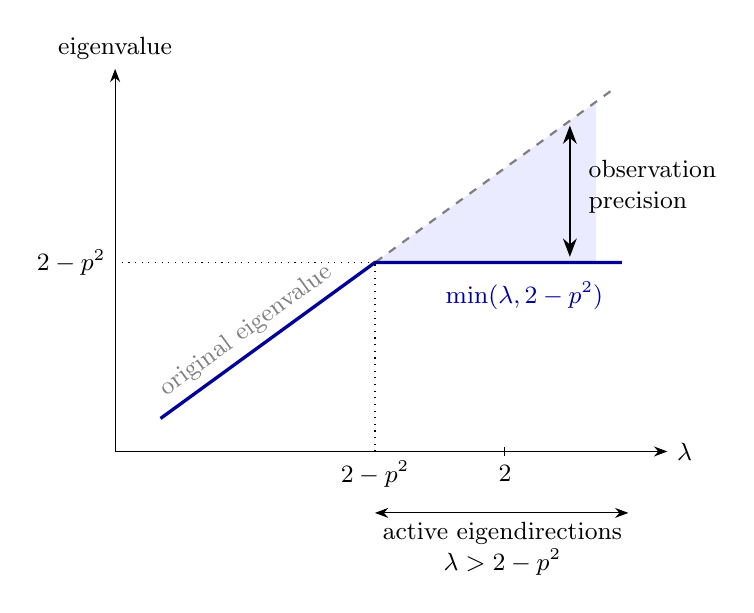
\begin{tikzpicture}[x=1.65cm,y=1.2cm,>=Stealth,font=\small]
 \fill[blue!8] (2,2)--(3.7,3.7)--(3.7,2)--cycle;
 \draw[->] (0,0)--(4.25,0) node[right] {$\lambda$};
 \draw[->] (0,0)--(0,4.05) node[above] {eigenvalue};
 \draw[gray,dashed,thick] (0.35,0.35)--(3.85,3.85);
 \draw[blue!60!black,very thick] (0.35,0.35)--(2,2)--(3.9,2);
 \draw[dotted] (2,0)--(2,2);
 \draw[dotted] (0,2)--(2,2);
 \node[below] at (2,0) {$2-p^2$};
 \node[left] at (0,2) {$2-p^2$};
 \draw (3,0.045)--(3,-0.045) node[below] {$2$};
 \node[gray,rotate=36,above] at (1.1,1.1) {original eigenvalue};
 \node[blue!60!black,below] at (3.15,1.9) {$\min(\lambda,2-p^2)$};
 \draw[<->,thick] (3.5,2.06)--(3.5,3.45);
 \node[right,align=left] at (3.57,2.8)
   {observation\\precision};
 \draw[<->] (2,-0.65)--(3.95,-0.65);
 \node[below,align=center] at (2.98,-0.65)
   {active eigendirections\\$\lambda>2-p^2$};
\end{tikzpicture}
\caption{A spectral cap, shown near the upper edge. The posterior interaction
$W_p$ retains eigenvalues below $2-p^2$ and flattens those above it.
The removed amount $(\lambda-(2-p^2))_+$ is the precision of the Gaussian
observation in that eigendirection. The drawing is schematic; its geometry
illustrates the defining spectral functions, not an eigenvalue density.}
\label{fig:spectral-cap}
\end{figure}


Observe
$h_p=B_pX+\mathsf N(0,B_p)$, with independent Gaussian increments as
$B_p$ increases, starting from zero precision if necessary.  Bayes' formula
makes the posterior interaction $W_p$ and the posterior field $h_p$.
Write $\mu_{p,h}$ for the cube posterior at a specified field $h$.  Let $\phi_p(h)$ be its log partition function,
$m_p(h)=\nabla\phi_p(h)$ its mean, and
$K_p(h)=P_p\nabla^2\phi_p(h)P_p$ its covariance restricted to $\cH_p$.
Superscript ${\rm sp}$ denotes the corresponding spherical quantities.
At path fields we often suppress the argument $h_p$.

On the joint space of the eigenframe and the spectral observation path,
the density of $\mathbf P$ relative to independent Haar measure and the
spherical observation law, through scale $p$, is
\begin{equation}\label{eq:source-4}
 L_p=\exp\{\phi_p(h_p)-\phi_p^{\rm sp}(h_p)\}.
\end{equation}
Indeed the likelihood of the observations is a common Gaussian factor
multiplied by the posterior partition function divided by the original one;
the factor $L_\circ$ cancels the two original partition functions.
The spin in spectral coordinates already has the spherical law by
Lemma~\ref{lem:edge-biased-law}; its observation noises are independent
Gaussian increments with covariance determined by the spectrum.  Hence the
entire spectral observation path under $\mathbf P$ has exactly its
spherical law.  We normalize its coordinates by
\[
 u_{p,a}=\frac{(U^{\mathsf T}h_p)_a}{p^2n^{1/3}},
 \qquad r=n^{-1/3+\delta},\qquad \delta=10^{-4}.
\]
We will use $r\le p\le p_{\rm top}$, allowing fixed-factor buffers at the
endpoints.  The values $d_a=p^2$ cause no discontinuity in the observations;
they may be omitted in scale integrals, and zero-variance coordinates are
omitted from density formulas.

\subsection{Saddles and cap estimates}

For a field $h\in\cH_p$, its spherical saddle $\alpha=\alpha_p(h)$ is
the unique solution above the pole of
\begin{equation}\label{eq:source-5}
 R_{p,\alpha}=(\max(d,p^2)+\alpha)^{-1},\qquad
 n=\Tr R_{p,\alpha}+\|R_{p,\alpha}h\|^2.
\end{equation}
The annulus $|\alpha_p(h)|\le s_0p^2$ is separated from zero field.  Its
radius as a function of $\alpha$ is
\[
 \ell_p(\alpha)=(p^2+\alpha)\sqrt{n-\Tr R_{p,\alpha}}.
\]
The following statement collects the precise Gaussian inputs needed later.
All upper cutoffs and tolerances in it are fixed constants before $n$ tends
to infinity.

\begin{proposition}[Cap inputs]\label{prop:edge-cap-inputs}
Fix a finite field radius $R$ and positive fixed error tolerances.  There
are sufficiently small constants $p_{\rm top},s_0>0$ such that the following
hold with probability tending to one in the range
$np^3\ge c\sqrt{\log n}$ and $p\le p_{\rm top}$.

\emph{Spectral and spherical estimates, at every scale.}
The spectral dimension satisfies $\dim\cH_p\asymp k_p$,
$d_1\ge-o(p^2)$ uniformly in the cap range, and
$\Tr R_{p,0}^2=O(n/p)$.  On $|\alpha|\le s_0p^2$,
$\ell_p(\alpha)\asymp p^2M_p$ and
$\ell_p'(\alpha)\asymp M_p$.  For
$\|h\|\le Rp^2M_p$, the saddle precision has gap comparable to $p^2$.
At $\alpha=\alpha_p(h)$, the density at $n$ of the squared norm of
$\mathsf N(R_{p,\alpha}h,R_{p,\alpha})$ is comparable to $\sqrt{p/n}$.
After multiplication by $e^{v^{\mathsf T}X}$ and renormalization, the
Gaussian mean becomes $R_{p,\alpha}(h+v)$ while its covariance remains
$R_{p,\alpha}$; its squared-norm density at $n$ is at most a fixed
multiple of $\sqrt{p/n}$.  For $m$ replicas, where $m$ is fixed, consider
rowwise linear or quadratic tilts that preserve Gaussianity.  The joint
density of their squared norms is at most $C_m(p/n)^{m/2}$ under the
following hypotheses.  The spectral rows remain independent after the rowwise tilt,
the tilted precision is positive definite, and on at least $ck_p$ rows
the post-tilt row covariance $C_a$ satisfies
$c p^{-2}\Id_m\preceq C_a\preceq C p^{-2}\Id_m$.
All comparison constants here are fixed.

\emph{Curvature estimates, at every scale.}
On the annulus, for any prescribed fixed $\epsilon_0>0$,
\begin{equation}\label{eq:source-6}
 K_p\preceq(1+\epsilon_0)p^{-2}\Id_{\cH_p},\qquad
 p^2(K_p)_{ee}\le1-\epsilon_1,
 \quad e=h/\|h\|,\quad \epsilon_1=0.1.
\end{equation}
On the entire field ball one also has $K_p\preceq C_Rp^{-2}\Id_{\cH_p}$,
where $C_R$ may be chosen before $\epsilon_0$.

\emph{Static comparisons and cube projection tails, on geometric lists.}
For any prescribed fixed geometric list of scales, uniformly over the field ball,
\[
 |\phi_p(h)-\phi_p^{\rm sp}(h)|\le\epsilon_v k_p,
 \qquad
 \|P_pm_p(h)-R_{p,\alpha_p(h)}h\|\le\epsilon_gM_p.
\]
Any fixed finite family of such lists is allowed.  For each
$h\in\cH_p$ with $\|h\|\le Rp^2M_p$, the cube posterior $\mu_{p,h}$
satisfies, uniformly for every $v\ge v_0$ with a sufficiently large fixed
threshold $v_0$,
\[
 \mu_{p,h}\{\|P_pX\|>vM_p\}\le C\exp(-ak_pv^6).
\]
For $v>p^{-1/2}$ the event is empty, since $\|X\|=\sqrt n$.
Here $a>0$, and the same bound holds under the uncapped zero-field cube
measure $\mu$ at the same list scales.

The spherical projection-tail estimate holds at every scale in the stated
range, for capped bounded-field and uncapped zero-field measures.  Also, at
every such cap scale, for independent
spherical replicas at a common field in the prescribed ball,
\[
 (\mu_{p,h}^{\rm sp})^{\otimes2}
 \{|n^{-1}X^{\mathsf T}X'|>\rho\}
 \le C\exp(-cn\rho^3),\qquad Cp\le\rho\le\rho_0,
\]
for a sufficiently small fixed $\rho_0>0$.  A fixed finite number of
replicas obeys the corresponding bound for any pair.
\end{proposition}

\begin{proof}[Source statements and the radial consequence]
The spectral, saddle, and density assertions are the conclusions of
\cite{CM}, Sections~15.2--15.3, ``Spectral estimates at the bottom
scale'' and ``Spherical saddles, norm densities, and tails.''  The static
comparison and its projection tails are Proposition~15.1 in that section.  Its order of choices is the one stated here:
fix the radius, errors, and geometric ratios, then decrease the upper cutoff.
The overlap estimate is the spherical estimate preceding that proposition.

The upper covariance bounds are Theorem~18.6, ``Uniform curvature of the true
cap potentials,'' in \cite{CM}.  Its lower endpoint is
$(\sqrt{\log n}/n)^{1/3}$, with fixed-factor changes permitted, so it
covers our scale $r$ and its fixed buffers.  We also use a consequence
retained in that theorem's proof.  Let $\gamma$ be the fixed geometric ratio chosen in that proof, and set
$R_{p,\alpha}^H=(P_pR_{p,\alpha}P_p)|_{\cH_p}$.  At an intermediate
evaluation ratio $x\in[\gamma^2,\gamma]$, Lemma~16.2, ``Evaluation with the induction
extension,'' in \cite{CM} bounds the radial entry of
$p^2(K_p-R_{p,\alpha}^H)$ above by $-0.26$.  The theorem's proof chooses
$s_0$ so that every target saddle lies inside the parent agreement annulus
with fixed slack, and applies exactly this deterministic evaluation.
Therefore
\[
 p^2(K_p)_{ee}\le\frac1{1+\alpha/p^2}-0.26
                  \le\frac1{1-s_0}-0.26\le0.9
\]
after decreasing $s_0$.  This proves the second part of
\eqref{eq:source-6} with a fixed tolerance.
\end{proof}

The list restriction in the static comparison is harmless, but its removal
requires a short argument because later observation identities integrate
over all scales.

\begin{lemma}[Interpolation between cap scales]
\label{lem:edge-static-interpolation}
The value, projected-mean, and cube projection-tail conclusions of
Proposition~\ref{prop:edge-cap-inputs} hold at every scale in the stated
range, after prescribing slightly smaller errors on a sufficiently fine
fixed geometric list and decreasing the upper cutoff.
\end{lemma}

\begin{proof}
First use an ordinary fixed-ratio list.  Monotonicity of $P_p$ and a
fixed-factor change in $M_p$ extend the uncapped projection tail to every
$p$.  Removing $B_p$ from the interaction changes its normalizing factor
by
\[
 \mu\exp(-X^{\mathsf T}B_pX/2)\ge
 \mu\{\|P_pX\|\le VM_p\}\,
       \exp(-\|B_p\|V^2M_p^2/2)\ge e^{-Ck_p},
\]
where $V$ is fixed and large.  We used $\|B_p\|=O(p^2)$ on the spectral
event.  Thus the projection tail persists at cap zero field.  A field
$\|h\|\le Rp^2M_p$ adds at most $Rk_pv$ on the shell
$\|P_pX\|=vM_p$; this is dominated by $ak_pv^6$ for large $v$.
The zero-field measure is even, so its linear-tilt normalizer is at least
one.  This gives the same tail on the field ball, with an adjusted
starting threshold.  The argument also bounds $\|P_qX\|/M_q$ under the
$p$-cap posterior whenever $q\ge p$ and $q/p$ is bounded: use the uncapped
$P_q$ tail, the same denominator lower bound, and $P_ph=h\in\cH_q$.
This is the tail needed to compare two nearby caps.  The spherical estimates give the identical conclusion.

Now choose a fixed geometric list with consecutive ratios close to one,
and let $q$ be its first scale above $p$.  Then $\cH_p\subset\cH_q$ and
\[
 \|W_p-W_q\|\le C(1-p/q)q^2,
 \qquad \operatorname{ran}(W_p-W_q)\subset\cH_q.
\]
For $h\in\cH_p$ in the prescribed ball, restrict first to
$\|P_qX\|\le VM_q$.  The change in log weight there is at most
$C(1-p/q)V^2k_q$.  On its complement, the projection tail controls the
exponential of the quadratic change: the exponent
$C(1-p/q)k_qv^2$ is dominated by the negative $ak_qv^6$ tail.
Choose $V$ first and the list ratio second.  The resulting log-partition
change is as small as desired in units $k_q$, for both cube and sphere.
Their value comparison at $q$ therefore implies the value comparison at
$p$, since $k_p/k_q$ is arbitrarily close to one.

For the mean, use the value comparison on a slightly larger field ball.
The frozen Gaussian saddle identity and its norm-density bound give, for
any unit $v\in\cH_p$ and both signs,
\[
 \log\mu_{p,h}e^{\pm t v^{\mathsf T}(X-R_{p,\alpha}h)}
       \le 2\epsilon_v k_p+\tfrac12t^2v^{\mathsf T}R_{p,\alpha}v+C.
\]
Jensen's inequality, with $t=\theta p^2M_p$, bounds the projected mean
discrepancy divided by $M_p$ by
$C\theta+(2\epsilon_v+C/k_p)/\theta$.  Choose $\theta$ from the required
mean tolerance and then $\epsilon_v$ sufficiently small.  This proves the
claim uniformly at every intermediate scale.
\end{proof}

The estimates of this section supply the ordinary Gaussian caps and the
spherical description of their observations.  The next section derives the
quantitative comparison and score estimates needed to retain the exact
$n^{2/3}$ time scale.

\section{Quantitative estimates for the observations}\label{sec:observations}

The coarse cap estimates of Proposition~\ref{prop:edge-cap-inputs} locate
the relevant fields and bound their covariance by a constant times $p^{-2}$.
For the time normalization in Theorem~\ref{thm:main}, we shall need a relative
covariance error that is integrable in logarithmic scale. The purpose of
this section is to obtain the averaged estimates from which that improvement
will follow. There are two different sources of smallness: a two-replica
comparison at the smallest observation scale, and an integrated likelihood
estimate at the larger scales.

We retain the notation and conditional-on-spectrum probability
$\mathbf P$ of Lemma~\ref{lem:edge-biased-law}. Thus $\mathbf P$ includes the
partition-function bias on the eigenframe and the ordinary Gibbs observation
path given that frame; $Q_\mu$ denotes the latter path law for fixed disorder.
Expectations with respect to these laws are denoted by $\mathbf E$ and
$Q_\mu[\,\cdot\,]$. Constants in the present section are uniform on each of
the tight spectral sets described in Remark~\ref{rem:edge-tight-convergence}.
They may depend on that set, on a fixed moment order, and on fixed field or
scale ratios. A bound $C\exp(-n^\xi)$ always has some $\xi>0$; decreasing
$\xi$ absorbs polynomial factors and the $O(\log n)$ scale intervals used
below. Recall that
\[
 r=n^{-1/3+\delta},\qquad \delta=10^{-4},\qquad k_p=np^3,
 \qquad M_p=(np)^{1/2}.
\]
All estimates involving a fixed multiplicative enlargement of the interval
of scales have the same meaning, provided its upper endpoint is sufficiently
small. In particular, $k_p$ grows as a positive power of $n$ throughout the
intervals considered here.

\subsection{Location of the path and coordinate moments}

The following estimate improves the fixed annulus test to a shrinking
annulus. It concerns the ordinary observation path averaged under
$\mathbf P$; it is not an assertion about every external field.

\begin{lemma}[The observation annulus]\label{lem:observations-annulus}
There are $a,\xi>0$ and a sufficiently small fixed upper scale
$p_{\mathrm{top}}>0$ such that
\begin{equation}\label{eq:source-7}
 |\alpha_p(h_p)|\le C k_p^{-a}p^2
 \qquad(r\le p\le p_{\mathrm{top}})
\end{equation}
outside a set of $\mathbf P$-probability at most $C\exp(-n^\xi)$.
On disorder events of probability arbitrarily close to one, the same
whole-path statement holds under $Q_\mu$, with a possibly smaller $\xi$.
\end{lemma}

\begin{proof}
Under $\mathbf P$, the field in spectral coordinates has exactly its
spherical distribution. Generate the spherical spin from independent
centered Gaussian coordinates $y_i$ of precision
$D_i'=d_i+b_n n^{-2/3}$, conditioned on $\sum_i y_i^2=n$; the choice of
$b_n$ is that of Proposition~\ref{prop:edge-conditioned-law}. Before this
conditioning, write
\[
 h_{p,i}=B_{p,i}y_i+B_{p,i}^{1/2}z_i,
 \qquad m=p^2+b_n n^{-2/3},
\]
where the $z_i$ are independent standard normals. On an active coordinate
$B_{p,i}=m-D_i'$, and direct expansion gives
\[
 \mathbf E_0\bigl(\|h_p\|^2-m^2\|y\|^2\bigr)
 =-m^2\Tr R_{p,b_n n^{-2/3}}.
\]
Here $\mathbf E_0$ denotes the unconditioned Gaussian expectation. The
subtraction of $m^2\|y\|^2$ removes the large contribution of the leading
coordinates: its coefficient on the standardized $y_i^2$ term is
$(B_{p,i}^2-m^2)/D_i'=D_i'-2m=O(p^2)$.

As a quadratic form in the standardized $(y,z)$ variables, the centered
quantity has squared Frobenius norm at most $Cp^4k_p$ and operator norm at
most $Cp^2k_p^{1/3}$. Indeed the cross coefficients are
$O(p^3/\sqrt{D_i'})$, while the spectral estimates give
\[
 \min_iD_i'\ge c n^{-2/3},\qquad
 \sum_{d_i\le p^2}(D_i')^{-1}\le Cnp.
\]
The inactive coordinates are bounded by the capped second resolvent trace.
The Gaussian quadratic-form exponential-moment formula therefore bounds
deviations larger than $p^2k_p^{9/10}$ by $C\exp(-k_p^{a_0})$ for some
$a_0>0$.

This estimate survives conditioning on $\|y\|^2=n$. To see this directly,
use the same exponential tilt in the Markov bound, with its parameter at
most one eighth of the inverse operator norm. The tilted joint Gaussian
covariance, and hence its $y$-marginal covariance, remain comparable to
the original ones. A fixed number of leading covariance eigenvalues bounds
the density of $n^{-2/3}\|y\|^2$ from above. Its original density at
$n^{1/3}$ is bounded below on the chosen spectral set, by
Proposition~\ref{prop:edge-conditioned-law}. The ratio of norm densities
therefore costs only a constant.

After conditioning, the deterministic target for $\|h_p\|^2$ is
$\ell_p(b_n n^{-2/3})^2\asymp p^2k_p$. The deviation just proved is a
relative $O(k_p^{-1/10})$ error, so it first places the inferred saddle
inside any fixed surrounding annulus for all sufficiently large $n$.
On that annulus,
the derivative of $\ell_p(\alpha)^2$ is comparable to $k_p$.
Consequently the preceding deviation bound implies
$|\alpha_p-b_n n^{-2/3}|\le Cp^2k_p^{-1/10}$. Since
$b_n n^{-2/3}/p^2=O(k_p^{-2/3})$, this proves the fixed-scale assertion.

For the whole path take a sufficiently fine inverse-polynomial mesh in
$p^2$. The functions $B_p$, the saddle targets, and their relevant
derivatives have polynomial bounds; the positive-part operation defining
$B_p$ is continuous at coordinate activations. Conditional on the spin,
each coordinate of the noise has independent Gaussian increments. A maximal
Gaussian estimate in every mesh interval, followed by a union bound over
coordinates and intervals, makes their oscillation smaller than the
polynomial tolerance just used. The fixed-scale exponential estimate
absorbs this union bound because $k_r=n^{3\delta}$. Finally,
Lemma~\ref{lem:edge-biased-law}, Markov's inequality, and $L_\circ\ge1/2$
outside a vanishing disorder exception transfer the result to $Q_\mu$.
\end{proof}

The signal-plus-noise representation also gives the moment estimates
needed to test the field against individual edge coordinates. Every
$u_{p,a}$ has moments of every fixed order bounded uniformly in $a,p$ under
$\mathbf P$. For each fixed finite set of leading indices and every fixed
$j<\infty$,
\begin{equation}\label{eq:source-8}
 \|u_{p,a}-x_a\|_{L^j(\mathbf P)}
 \le \frac{C_j}{pn^{1/3}},\qquad r\le p\le p_{\mathrm{top}}.
\end{equation}
Indeed the signal is $(B_{p,a}/p^2)x_a$ and the noise standard deviation is
at most $(pn^{1/3})^{-1}$. For a leading coordinate,
$|d_a|/p^2=O((pn^{1/3})^{-2})$. The same estimates hold in $L^j(Q_\mu)$
with tight disorder-dependent constants, simultaneously in $p$ in the sense
of moment bounds at each scale: apply the signal-plus-noise formula to the
tight quenched moments of $x_a$ furnished by the biased first moment and
the concentration of $L_\circ$.

\subsection{Two replicas and the smallest scale}

In the next lemma the field is deterministic in spectral coordinates.
Consequently $E_U$ means an independent Haar average at that fixed field,
whereas $\mathbf E$ subsequently averages a random field with its
spherical observation distribution.

\begin{lemma}[Replica comparison]\label{lem:observations-replicas}
Fix a bounded range for $\|h\|/(p^2M_p)$ and take the upper scale
sufficiently small. Uniformly for fields in this range,
\begin{equation}\label{eq:source-9}
 E_U L_p(h)^2\le \exp(C+Cnp^4).
\end{equation}
For a sufficiently large fixed $C_1$, the contribution to this normalized
second moment of cube pairs satisfying
$|n^{-1}X\cdot X'|>C_1p$ is at most $C\exp(-a k_p)$.
At $p=r$, the stronger estimates
\begin{equation}\label{eq:source-10}
 \begin{split}
 E_U(L_r-1)^2&\le Cn^{-1/4},\\
 E_U\!\left[L_r^2\|m_r-m_r^{\mathrm{sp}}\|^2\right]
 &\le C M_r^2 n^{-1/4}
 \end{split}
\end{equation}
hold for the full mean vectors, written in spectral coordinates. The first
bound also holds for the uncapped zero-field likelihood $L_\circ$.
The pair-tail assertion at scale $r$ also holds in that uncapped case.
\end{lemma}

\begin{proof}
Given the overlap $\rho=n^{-1}X\cdot X'$, the Haar angular integral of a
cube pair equals that of a spherical pair. The difference is entirely in
their overlap distributions. The replica Gram comparison of
\cite[Section~15.4, Equation~(15.10)]{CM} bounds the ratio on overlap cells
of width $2/n$ by $\exp(C+Cn\rho^4)$. Above $C_1p$ and below a small fixed
cutoff, the spherical pair tail costs $\exp(-a n\rho^3)$; choosing the
cutoff small pays for the comparison on all dyadic bands. At overlaps
bounded away from zero, the normalized zero-field comparison has a strictly
negative exponential rate, by
\cite[Section~15.4, p.~118]{CM}. A bounded
field changes logarithmic weights by at most $Cnp^{5/2}$, which preserves
that rate when the upper scale is small. Below $C_1p$ the comparison factor
is $\exp(C+Cnp^4)$. This proves \eqref{eq:source-9} and its pair-tail
assertion. The uncapped argument uses the corresponding uncapped spherical
tail from \cite[Section~15.3]{CM}.

We give the finer cell estimate, now taking $p=r$ throughout the remaining
comparison. On $|\rho|\le C_1p$, Stirling's formula and the spherical
overlap density show that the binomial mass of a cell and its spherical
mass differ by a relative error
\[
 O(np^4+p+n^{-1}).
\]
It remains to compare the angular integrands within one cell. Write a
spherical pair on an orthonormal sum-and-difference frame $(q,q')$. For
$A=W_p$ their tilt exponent is
\[
 \frac n2\bigl((1+\rho)q^{\mathsf T}Aq
 +(1-\rho){q'}^{\mathsf T}Aq'\bigr)
 +\sqrt{2n(1+\rho)}\,h^{\mathsf T}q.
\]
Its oscillation on a cell is bounded by
$C(|q^{\mathsf T}Aq-{q'}^{\mathsf T}Aq'|+p^{5/2})$.
This is uniformly bounded, and its average against the normalized tilted
spherical pair law on these cells is $O(p)$. For the latter assertion,
the exact identity
\[
 q^{\mathsf T}Aq-{q'}^{\mathsf T}Aq'
 =\frac{2Y^{\mathsf T}AY'
       -\rho(Y^{\mathsf T}AY+{Y'}^{\mathsf T}AY')}
       {n(1-\rho^2)}
\]
and $\|A\|\le C$ bound the diagonal terms by $C|\rho|$. It remains to show
\[
 E_{\mathrm{sp}}|Y^{\mathsf T}AY'|\le Cnp.
\]
At a bounded cap field, apply exponential Markov with parameter $cp^2$
to either sign of $Y^{\mathsf T}AY'$. The saddle means have squared norm
$O(np)$, the covariance trace-square is $O(n/p)$, and a sufficiently small
$c$ leaves a fixed precision margin. The Gaussian logarithmic moment
generating function is therefore at most $Ck_p$. Conditioning both norms
costs a constant by the joint norm-density bound in
\cite[Equation~(15.6)]{CM}. Integrating
the resulting tail, beginning at a sufficiently large multiple of $np$,
proves the displayed estimate. For uncapped zero field, freeze a Gaussian
parameter equal to a small fixed multiple of $p^2$. The same moment
generating function bound applies, and the deficit-filling lower density
estimate in that subsection costs at most $\exp(Ck_p)$; this gives the
same integrated bound.

For completeness, the passage from this averaged oscillation to comparison
of angular integrals does not require a pointwise $O(p)$ derivative bound.
The oscillation of the exponent on a cell is bounded by a fixed constant,
so the mean value theorem bounds the difference of its exponentials by a
constant times its integrated absolute derivative. The spherical overlap
density varies by a bounded factor on a cell. Summing over cells is thus
bounded by the preceding $O(p)$ integral. Slightly enlarging the overlap
cutoff pays for boundary cells by the pair tail.

At $p=r$, $np^4+p+n^{-1}=O(n^{-1/3+4\delta})=O(n^{-1/4})$.
The normalized pair integral consequently equals $1+O(n^{-1/4})$,
which proves the first part of \eqref{eq:source-10}, since $E_U L_r=1$.
Apply the same comparison with the test $n\rho$. Its absolute value on
the retained cells is at most $Cnp=CM_p^2$, and its change within one cell
is bounded by $2$. Hence
\[
 E_U\|L_rm_r\|^2
 =\|m_r^{\mathrm{sp}}\|^2+O(M_r^2n^{-1/4}).
\]
The first-moment identity $E_U[L_rm_r]=m_r^{\mathrm{sp}}$ turns this into
an $L^2$ bound on $L_rm_r-m_r^{\mathrm{sp}}$. Finally,
\[
 L_r(m_r-m_r^{\mathrm{sp}})
 =(L_rm_r-m_r^{\mathrm{sp}})-(L_r-1)m_r^{\mathrm{sp}},
\]
and $\|m_r^{\mathrm{sp}}\|\le CM_r$ proves the second part of
\eqref{eq:source-10}.
\end{proof}

\begin{corollary}[Cube edge marginals]\label{cor:observations-static}
Jointly with the spectral variables, in the sense of
Remark~\ref{rem:edge-tight-convergence}, the quenched cube integrals of
continuous cylinder functions of polynomial growth converge to their
integrals under $\Pi$. In particular, all fixed moments of any fixed finite
set of scaled edge coordinates converge.
\end{corollary}

\begin{proof}
In the uncapped comparison, insert a bounded Lipschitz cylinder function
of the scaled spectral coordinates in each replica numerator. Changing the
overlap within a cell moves each scaled coordinate by $O(n^{-5/6})$; the
preceding weight comparison therefore remains valid. The variance over Haar
frames of the numerator normalized by $Z_{\mathrm{sp}}$ tends to zero.
Together with $L_\circ\to1$ and
Proposition~\ref{prop:edge-conditioned-law}, this proves convergence of the
quenched cube cylinder integrals to $\Pi$. Polynomially growing continuous
tests follow by the higher moment bounds and truncation.
\end{proof}

\begin{corollary}[Mean moments and the initial score]\label{cor:observations-means}
For every fixed $j<\infty$, after reducing the fixed upper scale if needed,
\begin{equation}\label{eq:source-11}
 \mathbf E\bigl(\|m_p\|/M_p\bigr)^j
 +\mathbf E\bigl(\|m_p^{\mathrm{sp}}\|/M_p\bigr)^j\le C_j.
\end{equation}
At the smallest scale,
\begin{equation}\label{eq:source-12}
 \mathbf E\frac{\|m_r-m_r^{\mathrm{sp}}\|^2}{M_r^2}
 \le Cn^{-1/20},\qquad
 \mathbf E\|\nabla_{u_r}\log L_r\|^4=o(1).
\end{equation}
\end{corollary}

\begin{proof}
Lemma~\ref{lem:observations-annulus} confines the random field to a bounded
range except with power-exponential probability. At a fixed such field,
the Haar-averaged pair-tail numerator divided by the squared spherical
partition function is at most $Ce^{-ak_p}$, by
Lemma~\ref{lem:observations-replicas}.
Under the biased frame law $L_p\,dU$, the set
$L_p<e^{-ak_p/4}$ has mass at most $e^{-ak_p/4}$. On its complement,
the expectation of the posterior pair-tail probability is at most
$e^{ak_p/4}$ times that pair-tail integral. A further Markov bound gives
an exponentially small posterior pair tail outside an exponentially small
biased exception. Since
$\|m_p\|^2=\mu_{p,h}^{\otimes2}[X\cdot X']$, this implies
$\|m_p\|^2\le Cnp$ there. The deterministic bound $\|m_p\|\le\sqrt n$
pays for all exceptions and proves the cube part of
\eqref{eq:source-11}. The spherical part follows by the same argument.

For the first estimate in \eqref{eq:source-12}, split according to
$L_r\ge n^{-0.12}$. On this event \eqref{eq:source-10} bounds the biased
second moment by $CM_r^2n^{-0.13}$. The complementary biased probability
is at most $n^{-0.12}$; Cauchy--Schwarz and the fourth moment in
\eqref{eq:source-11} give $CM_r^2n^{-0.06}$. The field exceptions are
negligible. Finally
\[
 \nabla_{u_r}\log L_r
 =n^{1/3}r^2 P_r(m_r-m_r^{\mathrm{sp}}),\qquad
 n^{1/3}r^2M_r=n^{(5/2)\delta}.
\]
Interpolation of the decaying second moment with an arbitrarily high fixed
moment from \eqref{eq:source-11} proves the fourth-moment assertion.
\end{proof}

\subsection{Likelihood dissipation and covariance errors}

The smallest-scale comparison controls a single observation. At larger
scales the useful quantity is the score accumulated along the path.
The Gaussian observation construction is a form of stochastic localization
\cite{Eldan2013}; here, conditional on the disorder, the precision follows
the deterministic spectral schedule $B_p$. We derive its likelihood identity
below and combine it with the replica estimates just proved. Write
$a_p^{\mathrm{err}}=P_p(m_p-m_p^{\mathrm{sp}})$.

\begin{lemma}[Integrated score]\label{lem:observations-score}
There is a fixed $\tau>0$ such that, on each scale interval of a fixed
bounded ratio about $q$,
\begin{equation}\label{eq:source-13}
 \int\|a_p^{\mathrm{err}}\|^2\,d(p^2)
 \le Ck_q(q^\tau+k_q^{-\tau})
\end{equation}
outside a set of $\mathbf P$-probability at most $C\exp(-n^\xi)$.
The bound holds simultaneously on a geometric list of intervals, with
fixed enlargements, and also holds in expectation.
\end{lemma}

\begin{proof}
Use $t=p^2$ as the channel parameter and take the filtration generated by
the eigenframe and observations through time $t$. In particular, every
disorder event is measurable at time zero. Between coordinate activations,
$\dot B_t=P_p$, and the Gaussian likelihood identity gives
\[
 d\log L_p=a_p^{\mathrm{err}}\cdot d\mathcal B_t
       +\tfrac12\|a_p^{\mathrm{err}}\|^2dt,
\]
where $\mathcal B$ is the innovation Brownian motion in the active
subspace. The bracket of the martingale is the score integral. There is
no singular term at an activation because the added precision starts at
zero. These statements also follow by It\^o differentiation of the
posterior partition function, including the compensating interaction
change $-dB_t$.

Put $H_q=Ck_q(q^\tau+k_q^{-\tau})$, with $\tau$ small and fixed.
At the first endpoint, the likelihood-density identity gives
$\mathbf P(\log L_p<-H_q)\le e^{-H_q}$. At the last endpoint,
\eqref{eq:source-9} gives
\[
 \mathbf P(\log L_p>H_q,\ h_p\text{ in the bounded range})
 \le \exp(-H_q+C+Ck_q q).
\]
Choose $C$ large and use Lemma~\ref{lem:observations-annulus} outside
the range. An exponential martingale inequality now bounds the event
that the bracket exceeds a sufficiently large multiple of $H_q$ while
these endpoint inequalities hold. This proves
\eqref{eq:source-13}. The logarithmic number of intervals is absorbed
by the power-exponential bound. Both means have norm at most $\sqrt n$,
so the integral has a polynomial deterministic bound; integrating the
exception proves the expectation assertion.
\end{proof}

Let $\mathcal G_n$ be the intersection of the disorder events on which
the fixed-tolerance annular covariance bounds of
Proposition~\ref{prop:edge-cap-inputs}, the static value and projected-mean
comparisons of Lemma~\ref{lem:edge-static-interpolation}, and the associated
projection tails hold on the full scale and fixed field ranges used below.
All tolerances and ranges are fixed before taking $n\to\infty$; their
finite intersection has probability tending to one.
The next estimate is asserted on $\mathcal G_n$; its exceptional probability
is measured before any conditioning on that event.

\begin{lemma}[Integrated covariance error]\label{lem:observations-curvature}
Put $D_p^K=p^2K_p-\Id$ on $\mathcal H_p$. After decreasing $\tau>0$ if
necessary,
\begin{equation}\label{eq:source-14}
 \int_q^{2q}\frac{\|D_p^K\|_{\mathrm F}^2}{k_p}\,d\log p
 \le C(q^\tau+k_q^{-\tau})
\end{equation}
outside an event whose intersection with $\mathcal G_n$ has
$\mathbf P$-probability at most $C\exp(-n^\xi)$. Fixed enlargements of
the interval are allowed, and the assertions hold simultaneously on a
geometric list.
\end{lemma}

\begin{proof}
On the shrinking annulus of Lemma~\ref{lem:observations-annulus}, the
spherical covariance has norm $O(p^{-2})$. By rotation invariance within
the flat cap its restriction to $e^\perp$, $e=h_p/\|h_p\|$, is scalar.
The frozen Gaussian linear-tilt bound gives an $O(p^{-1})$ error between
the spherical radial mean and the saddle mean. Dividing by
$\|h_p\|\asymp p^2M_p$ shows that the transverse covariance differs
from $(p^2+\alpha_p)^{-1}\Id$ by $O(p^{-2}k_p^{-1/2})$.
The remaining radial covariance is rank one. Thus its contribution,
and the shrinking saddle parameter, are already bounded by the right
side of \eqref{eq:source-14}.

It remains to compare $K_p$ and $K_p^{\mathrm{sp}}$. The spherical
posterior, evaluated along the cube observation path, has innovation
drift $K_p^{\mathrm{sp}}a_p^{\mathrm{err}}dt$. Subtracting the two
posterior mean equations gives
\[
 da_p^{\mathrm{err}}
 =(K_p-K_p^{\mathrm{sp}})\,d\mathcal B_t
       -K_p^{\mathrm{sp}}a_p^{\mathrm{err}}dt
\]
between activations. Multiply $p^2\|a_p^{\mathrm{err}}\|^2$ by a smooth
nonnegative cutoff supported on an enlarged scale interval and equal to
one on $[q,2q]$, with bounded derivative in $\log p$. It\^o's formula
and integration by parts give
\[
 \int_q^{2q}\|p^2(K_p-K_p^{\mathrm{sp}})\|_{\mathrm F}^2\,d\log p
 \le C\int_{\mathrm{enlargement}}\|a_p^{\mathrm{err}}\|^2\,d(p^2)
       +C|\mathcal M|.
\]
Activations add squared new mean coordinates with nonnegative coefficients,
so they may be discarded on this side of the inequality. The cutoff is
zero at both endpoints; the displayed energy identity is applied over the
entire interval, not at a stopping time. Its martingale is
\[
 \mathcal M=2\int\chi(t)t
   \langle a_{\sqrt t}^{\mathrm{err}},
      (K_{\sqrt t}-K_{\sqrt t}^{\mathrm{sp}})\,d\mathcal B_t\rangle.
\]
For concentration, stop this stochastic integral alone at the first
failure of the annular covariance bounds, and set its integrand to zero
on $\mathcal G_n^c$, a time-zero event. Its bracket is then bounded by
$C\int\|a_p^{\mathrm{err}}\|^2d(p^2)$. The stopped integral agrees with
$\mathcal M$ on $\mathcal G_n$ and the whole-path annulus event.
The martingale inequality, Lemma~\ref{lem:observations-score}, and
Lemma~\ref{lem:observations-annulus} therefore prove the assertion.
Division by $k_q\asymp k_p$ gives the stated normalization.
\end{proof}

We finish with an angular estimate that will identify derivatives of the
limiting measure. This estimate uses the remaining Haar randomness without
restricting first to $\mathcal G_n$.

\begin{lemma}[Angular score]\label{lem:observations-angular}
For a cap field $h$, write $\widetilde h=U^{\mathsf T}h$ and
$\widetilde\phi_p(\widetilde h)=\phi_p(U\widetilde h)$.
Let $A$ be a fixed skew-symmetric matrix supported on finitely many leading
spectral coordinates, and set
$\mathcal R=(A\widetilde h)\cdot\nabla_{\widetilde h}$. There is
$\tau'>0$ such that
\begin{equation}\label{eq:source-15}
 \int_q^{2q}
 \frac{\mathbf E|\mathcal R\widetilde\phi_p(\widetilde h_p)|^2}
      {n^{2/3}p^2}\,d\log p
 \le C_A(q^{\tau'}+k_q^{-\tau'}).
\end{equation}
\end{lemma}

\begin{proof}
The coordinates on which $A$ acts belong to the cap for all sufficiently
large $n$.
By \eqref{eq:source-4}, the joint density of the frame and spectral
observation relative to independent Haar and the spherical observation
law is $L_p$. Condition on the physical capped matrix $W_p$, the physical
vector $h_p$, and the spectral coordinates of that vector. The spherical
observation density is now fixed, and $L_p$ depends only on the fixed
physical data and spectrum. The remaining rotation of the spectral frame
in $e^\perp\cap\mathcal H_p$ is therefore exactly Haar. In physical
coordinates, the differentiation direction is $UA\widetilde h_p$, which
is orthogonal to $h_p$ and has length $|A\widetilde h_p|$. The spherical
mean in the cap is radial. Haar averaging consequently gives
\[
 \frac{\mathbf E|\mathcal R\widetilde\phi_p(\widetilde h_p)|^2}
      {n^{2/3}p^2}
 \le C\mathbf E\left[
 |Au_p|^2\frac{p^2\|a_p^{\mathrm{err}}\|^2}{k_p}\right].
\]
Apply \eqref{eq:source-13} in expectation and interpolate with the higher
moments in \eqref{eq:source-11} and the coordinate moments following
Lemma~\ref{lem:observations-annulus}. H\"older's inequality on probability
times logarithmic scale gives \eqref{eq:source-15}, with a smaller positive
exponent. No event depending on the unused spectral refinement was inserted
before the Haar average.
\end{proof}

\section{Conditional variance at the exact cap scale}\label{sec:variance}

The observation removes the part of a test that depends on the leading
spectral coordinates. We now show that its remaining variance costs at most
$Cp^{-2}$ times the original heat-bath energy. The exponent $2$ is essential:
integrating a covariance bound $(1+\varepsilon)p^{-2}$ with a fixed
$\varepsilon>0$ would instead produce a power loss. The integrated estimates
of Section~\ref{sec:observations} allow us to replace this fixed error by
one that is integrable in logarithmic scale.

\begin{proposition}[Conditional variance]\label{prop:variance-main}
There is a fixed $p_*>0$ with the following property. For every
$\varepsilon>0$ there are finite constants $C$, $\xi>0$ and disorder events
$\mathcal V_n$ with $\liminf_n\mathbb P(\mathcal V_n)\ge1-\varepsilon$
such that, on $\mathcal V_n$, simultaneously for every real function $f$
on the cube and every $r\le p\le p_*$,
\begin{equation}\label{eq:source-16}
 V_p(f):=Q_\mu[\Var(f\mid h_p)]
 \le Cp^{-2}\cE(f)+Ce^{-n^\xi}\|f\|_\infty^2.
\end{equation}
The constants and the disorder event are independent of $f$. The inequality
also holds componentwise and may be summed for vector-valued functions.
\end{proposition}

In particular, the remainder is negligible for any fixed polynomial bound
on the supremum norm, including for disorder-dependent tests. We first
prove the requisite covariance improvement, then establish a variance bound
at a fixed upper scale, and finally integrate the posterior variance identity.

\subsection{A sharper upper covariance bound}

We work initially on the disorder event $\mathcal G_n$ of
Section~\ref{sec:observations}. Its fixed tolerances will be chosen below;
no tolerance depends on $n$. Probabilities in the next proposition are
measured under $\mathbf P$ before restriction to this event.

\begin{proposition}[Positive covariance error]\label{prop:variance-curvature}
There are fixed $a,\xi,C>0$ and a sufficiently small fixed $p_*>0$ such
that, for each deterministic $p\in[r,p_*]$ away from the activation
scales,
\begin{equation}\label{eq:source-17}
 p^2K_p\preceq\bigl(1+C(p^a+k_p^{-a})\bigr)\Id
\end{equation}
outside an event $\mathcal N_{n,p}$ satisfying
$\mathbf P(\mathcal N_{n,p}\cap\mathcal G_n)\le Ce^{-n^\xi}$.
The exceptional event may depend on $p$; its probability bound has common
constants for the entire scale range. By Fubini's theorem the same bound
holds after integration in $d\log p$, with a possibly smaller $\xi$.
\end{proposition}

The gain comes from comparing a small cap to a larger one. The radial
covariance deficit permits us to put all positive errors in the tangent
space of the parent field. Their restriction to the much smaller child
space is then controlled by the unused Haar rotation.

Fix a small constant $\gamma>0$, a child scale $c$, and a parent scale $p$
such that $x=c/p\in[\gamma,2\gamma]$. Put $\Delta=B_p-B_c$.
Conditional on $h_c$, the parent field has the transition law
\[
 d\mathsf T_{c,p,h_c}(y)
 =\frac{e^{\phi_p(y)}\,dN(h_c,\Delta)(y)}
        {\int e^{\phi_p(z)}\,dN(h_c,\Delta)(z)}.
\]
The Gaussian is taken on the positive-increment space. The observation
precision increment, compressed to the child space, is
$\Delta_c=(P_c\Delta P_c)|_{\mathcal H_c}=(1-x^2)p^2\Id$.
Writing $[M]_{\mathcal H_c}$ for this compression of any operator $M$,
differentiation of the Gaussian convolution gives
\begin{equation}\label{eq:source-18}
 K_c=\Delta_c^{-1}
       [\Cov_{\mathsf T_{c,p,h_c}}(h_p)]_{\mathcal H_c}\Delta_c^{-1}
        -\Delta_c^{-1}.
\end{equation}

\begin{lemma}[An annular extension for the transition]\label{lem:variance-extension}
Choose $\eta>0$ sufficiently small compared with $\gamma^2$, then the
coarse curvature tolerance $\varepsilon_0$ sufficiently small compared with
$\eta$. The annulus width $s_0$ and the fixed upper scale may be chosen
so that the following holds on $\mathcal G_n$. For every child field with
$|\alpha_c(h_c)|\le s_0c^2$, the parent potential has an extension
$\overline\phi_p$ with upper Hessian bound $(1+\eta)p^{-2}\Id$ that agrees
with $\phi_p$ near $|\alpha_p|\le s_0p^2/2$. Under both the true transition
and the transition obtained by using $\overline\phi_p$, the complement of
this agreement region has probability at most $Ce^{-a_1k_p}$. The same
bound holds with any fixed polynomial moment of
$\|h_p\|/(p^2M_p)$ inserted, after decreasing $a_1>0$.
\end{lemma}

\begin{proof}
We give the construction and its tail comparison, following the cap
extension method of \cite[Proposition~16.1]{CM}. On
$|\alpha_p|\le3s_0p^2/4$, take the infimum of the quadratics
\[
 \phi_p(z)+\nabla\phi_p(z)\cdot(y-z)
             +\frac{1+\eta}{2p^2}\|y-z\|^2.
\]
Each of these supports lies above $\phi_p$ on that smaller annulus.
Choose $s_0$ small compared with $\eta$ and $\gamma^2$. The radial buffer
between the smaller and larger annuli then determines a fixed
$\beta_{\mathrm{buf}}>0$ such that every segment starting in the smaller
annulus and of length at most $\beta_{\mathrm{buf}}p^2M_p$ remains in
the larger one. For such pairs $y,z$, the supporting inequality follows
by integrating the coarse Hessian bound along their segment.
For $d=y-z$ with $\|d\|\ge\beta_{\mathrm{buf}}p^2M_p$, freeze the
spherical saddle at $z$. The frozen Gaussian bound bounds the spherical
logarithmic increment by the quadratic with Hessian
$(p^2+\alpha_p(z))^{-1}\Id$, its saddle gradient, and a bounded density
error. The static value and gradient errors from
Lemma~\ref{lem:edge-static-interpolation} are at most
$\epsilon_v k_p$ and $\epsilon_gM_p$. Relative to $\|d\|^2/p^2$, their
combined contribution, including the density error, is at most
\[
 \frac{2\epsilon_v+C/k_p}{\beta_{\mathrm{buf}}^2}
       +\frac{\epsilon_g}{\beta_{\mathrm{buf}}}.
\]
The frozen Hessian is at most $(1+Cs_0)p^{-2}\Id$. Thus, after choosing
$s_0$, then $\beta_{\mathrm{buf}}$, then the static errors, the excess
quadratic term dominates this residual for all sufficiently large $n$.
This proves the supporting property,
and the infimum is a semiconcave extension agreeing on the smaller annulus.

For the transition tails freeze instead the child saddle
$\alpha=\alpha_c(h_c)$. As reference use the Gaussian transition tilted
by the parent quadratic $\|y\|^2/(2(p^2+\alpha))$ with no linear term.
Writing $R_u=R_{u,\alpha}$, its law is characterized by
\[
 R_ph_p\sim N(R_ch_c,R_c-R_p),
 \qquad R_c^{-1}=R_p^{-1}-\Delta.
\]
Since the child saddle satisfies its norm constraint, the expected squared
norm of $h_p$ is $\ell_p(\alpha)^2$. Its covariance norm is at most
$C\gamma^{-2}p^2$. Therefore deviations in radius by $vp^2M_p$ cost
\[
 C\exp(-a_0\gamma^2k_pv^2),
 \qquad v\ge C(\gamma\sqrt{k_p})^{-1}.
\]
The radius $\ell_p(\alpha)$ lies strictly inside the parent agreement
annulus, because $|\alpha|\le s_0c^2$.

Calibrate the reference quadratic to the spherical potential at this
radius. On a bounded range of scaled radii the true potential is at most
the reference quadratic plus $\epsilon k_p+O(1)$, with arbitrarily small fixed
$\epsilon>0$, by the frozen norm-density bound and static comparison.
Outside a sufficiently large bounded range, the zero-field projection
tail gives
\[
 \phi_p(y)-\phi_p(0)
 \le Ck_p\left(1+
       \left(\frac{\|y\|}{p^2M_p}\right)^{6/5}\right).
\]
This follows by integrating the tail
$\exp(-ak_pv^6)$ against the linear field tilt. Its growth is absorbed
by the reference quadratic. For the extension, use the support centered
at the point of radius $\ell_p(\alpha)$ in the direction of $y$.
At radial distance $vp^2M_p$ its excess above the reference is at most
\[
 \epsilon k_p+\epsilon k_pv+C(\eta+s_0)k_pv^2+O(1).
\]
Choose $\eta+s_0$ small compared with $\gamma^2$, and choose
$\epsilon$ after the fixed gap to the boundary of agreement. These errors
are strictly smaller than the Gaussian deviation cost outside agreement.

The normalizing integrals relative to the reference are bounded below
by $\exp(-\epsilon'k_p)$ with any needed fixed $\epsilon'>0$.
Indeed integrate over a sufficiently thin fixed relative shell around
$\ell_p(\alpha)$. Both potentials agree there, their values at the
central radius are given by static comparison, and their gradients are
bounded in units of $M_p$. Gaussian concentration gives a positive lower
bound for the reference mass of this shell for large $n$. This proves
the asserted transition tails; polynomial moments are absorbed by the
same Gaussian deviation estimate and the subquadratic bound above.
\end{proof}

The extension permits Brascamp--Lieb's covariance inequality
\cite{BrascampLieb1976} to be used in the Gaussian convolution. After
whitening, the transition has a fixed strict log-concavity margin depending
on $\gamma$, because
$\Delta\preceq(1-x^2)p^2\Id$ and $\eta\ll\gamma^2$. If $K$ denotes
the extended Hessian, this inequality bounds its covariance by the
expectation of
\[
 \Delta^{1/2}
 (\Id-\Delta^{1/2}K\Delta^{1/2})^{-1}\Delta^{1/2}.
\]
Mollification justifies this formula for the semiconcave extension.
Lemma~\ref{lem:variance-extension} then replaces the extended Hessian by
the true one inside agreement and replaces the extended transition by
the true transition, with exponentially small errors. The covariance
comparison includes the means: Cauchy--Schwarz and the polynomial moment
tail bound control the difference of first and second moments. In
\eqref{eq:source-18}, only $\Delta_c$ is inverted outside this expression,
so newly activated directions of arbitrarily small precision cause no loss.

\begin{lemma}[Removing the radial error]\label{lem:variance-radial}
On the coarse annulus, let $D=p^2K_p-\Id$, $e=h_p/\|h_p\|$,
$z=D_{\perp e}$, and define, on $e^\perp$,
\[
 E_p=(D_{\perp\perp}+zz^{\mathsf T}/|D_{ee}|)_+,
\]
extended by zero on $e$. Put $s_p^+=\|D_+\|$. Then
$D\preceq E_p$ and
\begin{equation}\label{eq:source-19}
 \|E_p\|\le Cs_p^+,
 \qquad
 \frac{\Tr E_p}{k_p}
 \le C\frac{\|D\|_{\mathrm F}}{\sqrt{k_p}}+\frac C{k_p}.
\end{equation}
\end{lemma}

\begin{proof}
The coarse radial deficit gives $D_{ee}\le-\varepsilon_1<0$.
For each transverse vector, maximize the quadratic form of $D$ over its
radial coordinate. The resulting form is
$D_{\perp\perp}+zz^{\mathsf T}/|D_{ee}|$, proving $D\preceq E_p$.
Since $K_p\succeq0$ and $p^2K_p\preceq(1+\varepsilon_0)\Id$, both
$D$ and the maximizing radial coordinate for a unit transverse vector
are bounded by constants. Comparing that vector with
$D\preceq s_p^+\Id$ proves the norm estimate. The trace of the rank-one
correction is bounded, while the trace of the positive part of
$D_{\perp\perp}$ is at most
$\sqrt{\dim\mathcal H_p}\,\|D\|_{\mathrm F}$. This proves
\eqref{eq:source-19}.
\end{proof}

Define $E_p=0$ outside the coarse annulus, and also whenever the local
covariance inequalities needed in Lemma~\ref{lem:variance-radial} fail.
This definition uses only the physical parent data $(W_p,h_p)$ and the
spectrum. In particular, it is defined and bounded before imposing
$\mathcal G_n$. On that event, the local failures never occur on the
annulus. By choosing $\varepsilon_0$ small enough, we have
$\|E_p\|\ll\gamma^2$.

Insert $K_p\preceq p^{-2}(\Id+E_p)$ in the covariance comparison.
The baseline $p^{-2}\Id$ gives $c^{-2}\Id$ in
\eqref{eq:source-18}. For the correction, expand the inverse around
$\Id-\Delta/p^2$. Its inverse has norm at most $x^{-2}$; because
$\|E_p\|\ll x^2$, the whole positive correction is at most twice the
first insertion in quadratic-form order. On the child subspace the two
outer inverse factors are scalars. Multiplication by $c^2$ yields
\begin{equation}\label{eq:source-20}
 s_c^+\le Cx^{-2}\mathsf T_{c,p,h_c}
                    [\|P_cE_pP_c\|]+C_\gamma e^{-a_1k_p}
\end{equation}
for every child field in its annulus. The first constant is absolute.

\begin{lemma}[Compression by the unused frame]\label{lem:variance-compression}
For $x=c/p\in[\gamma,2\gamma]$,
\begin{equation}\label{eq:source-21}
 \|P_cE_pP_c\|
 \le C\left(\frac{\Tr E_p}{k_p}+x^3\|E_p\|\right)
\end{equation}
outside a set of $\mathbf P$-probability at most
$C\exp(-a_\gamma k_p)$. This is an unconditional assertion with respect
to the unused spectral refinement; its exceptional set may afterwards
be intersected with $\mathcal G_n$.
\end{lemma}

\begin{proof}
Condition on $W_p$, the physical field $h_p$, and its spectral coordinates,
as in Lemma~\ref{lem:observations-angular}. The remaining frame in
$e^\perp\cap\mathcal H_p$ is Haar, and $E_p$ is fixed under this
conditioning. For a uniformly rotating unit vector $v$ in that space,
the Gaussian representation of the uniform sphere gives
\[
 \mathbb P\left(v^{\mathsf T}E_pv>
   \frac{C(\Tr E_p+t\|E_p\|)}{k_p}\right)
 \le C(e^{-t}+e^{-c_0k_p}).
\]
The same bound applies to a fixed vector of norm at most one. Choose a
constant-resolution net of the child unit sphere and project it onto
$e^\perp$. Its cardinality is at most
$\exp(C\dim\mathcal H_c)\le\exp(Cx^3k_p)$. With
$t=C_2x^3k_p$, a sufficiently large $C_2$ pays for the net; taking
$\gamma$ sufficiently small also pays for the second exponential term.
The net approximation for a positive quadratic form proves
\eqref{eq:source-21}.
\end{proof}

\begin{proof}[Proof of Proposition~\ref{prop:variance-curvature}]
Let $\widehat s_p$ be $s_p^+$ on the full coarse annulus and zero
outside it. We now restrict to $\mathcal G_n$. Average
\eqref{eq:source-20} over
$c/(2\gamma)\le p\le c/\gamma$ with normalized logarithmic measure,
and condition on $W$ and the observation path through $c$.
Combining \eqref{eq:source-19} and \eqref{eq:source-21}, the operator-norm
term has coefficient at most $Cx^{-2}x^3\le C\gamma$.
Choose $\gamma$ so that this coefficient, denoted by $\theta$, is less
than $1/2$. The trace term is controlled by Cauchy--Schwarz and the
integrated Frobenius estimate \eqref{eq:source-14}. We obtain
\begin{equation}\label{eq:source-22}
 \widehat s_c\le
 \theta\operatorname{avg}_{c/(2\gamma)\le p\le c/\gamma}
    \mathbf E[\widehat s_p\mid W,\mathcal F_c]
 +C_\gamma(c^{b}+k_c^{-b})+\operatorname{err}_c,
\end{equation}
where $b>0$, $\mathcal F_c$ is the observation filtration, and
$\operatorname{err}_c\ge0$ satisfies
\[
 \mathbf E[\mathbf1_{\mathcal G_n}\operatorname{err}_c]
 \le Ce^{-n^\xi}
\]
uniformly at deterministic scales. To verify the exceptional terms in
this assertion, first apply \eqref{eq:source-14} to the parent scale
integral before taking its conditional expectation. Its failures and
those of \eqref{eq:source-21} have exponential probability and at most
polynomial cost. Since $W$ is included in the conditioning, the indicator
of $\mathcal G_n$ commutes with that conditional expectation. No assertion
of Haar independence conditional on $\mathcal G_n$ is used. If the child
field is outside its annulus, the inequality holds by truncation.

Choose $a\le b$ sufficiently small that $\theta\gamma^{-a}<1$.
For a sufficiently large $C'$, the function
$b_0(c)=C'(c^a+k_c^{-a})$ dominates its parent average multiplied by
$\theta$, plus $C_\gamma(c^b+k_c^{-b})$, with a fixed margin.
It also dominates the coarse constant bound at the upper scales where
the parent interval no longer fits below $p_*$. Take positive parts
above $b_0$ in \eqref{eq:source-22}, use conditional Jensen, and average
over $\mathbf P$ with $\mathbf1_{\mathcal G_n}$. At each iteration the
scale increases by at least $(2\gamma)^{-1}>1$, so there are only
$O(\log n)$ generations; their errors sum to at most
$Ce^{-n^\xi}\sum_{j\ge0}\theta^j$. Thus
\[
 \mathbf E[\mathbf1_{\mathcal G_n}
       (\widehat s_c-b_0(c))_+]\le Ce^{-n^\xi}.
\]
Enlarging $C'$ and applying Markov's inequality proves the asserted
probability bound, since $b_0(c)$ is bounded below by an inverse
polynomial on the scale range. Lemma~\ref{lem:observations-annulus}
removes the truncation. All bounds were uniform at deterministic scales,
so Fubini's theorem gives their integrated version.
\end{proof}

\subsection{The variance bound at a fixed upper scale}

We next obtain the starting variance estimate from the fixed-scale
continuation in \cite[Section~19.4]{CM}. We record precisely why its
entropy estimate applies to the perturbations needed here.

\begin{lemma}[The fixed-scale starting bound]\label{lem:variance-start}
On disorder events of probability tending to one, for a sufficiently
small fixed $p_{\mathrm{top}}>0$ and every real function $f$ on the cube,
\[
 V_{p_{\mathrm{top}}}(f)
 \le C\cE(f)+Ce^{-a n}\|f\|_\infty^2.
\]
The event and constants are independent of $f$.
\end{lemma}

\begin{proof}
The continuation in \cite[Section~19.4]{CM} increases the observation
precision from $B_{p_{\mathrm{top}}}$ through finitely many cap intervals,
a bridge to a classical field, and a bounded-duration continuation to
a diagonal-interaction endpoint. For an initial change of spin law from
$\mu$ to $\nu$, let $\nu_s,\mu_s$ be the two posteriors, let
$l_s=D(\nu_s\Vert\mu_s)$, and put
$H(s)=E_{Q_\nu}l_s$. On this continuation, the estimate used is
\begin{equation}\label{eq:variance-entropy-ode}
 \dot H(s)\ge-CH(s)-e^{-a n}.
\end{equation}
This is \cite[Equation~(19.17)]{CM}. Its proof uses upper bounds on
observation likelihoods and posterior entropy tails, rather than a
support restriction on the posterior. We explain its application when
the initial density lies between $1/2$ and $2$. Every observation likelihood
then has the same bounds, every posterior density ratio lies between
$1/4$ and $4$, and $l_s\le\log4$.

At the classical part, the ordinary posterior covariance is bounded on
a fixed normalized field neighborhood outside an event of probability
$e^{-an}$; farther along the continuation it is bounded for every field.
The linear entropy inequality in that neighborhood gives
$\|m_\nu-m_\mu\|^2\le Cl_s$ whenever $l_s$ is bounded: a trial field
shift of size proportional to $\sqrt{l_s}$ fits the neighborhood.
The bounded density ratios pay for the ordinary exceptional paths.

To propagate this mean estimate across a preceding cap or bridge
interval, use the approximate gradient $g_s$ furnished by the extended
potential there. The transport identity
\cite[Lemma~18.3]{CM} holds under either initial law. If $U$ is its
linear transport from the current time $s$ to the end of the interval,
subtraction gives, for a vector $v$ in the current rate subspace,
\begin{align*}
 \langle v,m_{\nu,s}-m_{\mu,s}\rangle
 ={}&E_{Q_{\nu,h}^{\mathrm{cont}}}
       \langle Uv,m_{\nu,\mathrm{end}}-m_{\mu,\mathrm{end}}\rangle\\
 &+(E_{Q_{\nu,h}^{\mathrm{cont}}}
       -E_{Q_{\mu,h}^{\mathrm{cont}}})
       \langle Uv,m_{\mu,\mathrm{end}}-g_{\mathrm{end}}\rangle.
\end{align*}
Here the two continuation laws live on the same path space, and the same
path function $U$ is used in both expectations. Its operator norm is
bounded by a fixed constant on these fixed intervals. At agreement,
the terminal approximation error in the tested subspace has bounded
norm. Truncate it there. Data processing gives
$D(Q_{\nu,h}^{\mathrm{cont}}\Vert Q_{\mu,h}^{\mathrm{cont}})\le l_s$,
so Pinsker's inequality bounds the second term by
$C\sqrt{l_s}\|v\|$.

The complements have exponentially small averaged squared cost. Indeed,
for any nonnegative terminal cost $W_1$, the bounded full-path and
prefix likelihoods give both
\[
 E_{Q_\nu}E_{Q_{\nu,h}^{\mathrm{cont}}}W_1
 \le C E_{Q_\mu}W_1,
 \qquad
 E_{Q_\nu}E_{Q_{\mu,h}^{\mathrm{cont}}}W_1
 \le C E_{Q_\mu}W_1.
\]
Apply these inequalities to the polynomially weighted ordinary
exceptions in the terminal approximation estimates of
\cite[Section~19.4]{CM}. Conditional Cauchy--Schwarz controls the first
transport term by the terminal squared mean difference. Taking the
supremum over unit $v$ costs no dimension factor because all the bounds
are norm bounds uniform in $v$. Since terminal expected posterior entropy
is at most $H(s)$, backward induction through the finite list yields
\[
 E_{Q_\nu}\|P_{\mathrm{rate}}
                   (m_{\nu,s}-m_{\mu,s})\|^2
 \le CH(s)+Ce^{-a n}.
\]
The observation entropy identity
\cite[Lemma~19.2]{CM}, with bounded precision rates on these intervals,
now proves \eqref{eq:variance-entropy-ode}. This also proves that its
constants apply uniformly to the bounded-density perturbations below.

Normalize $\|f\|_\infty\le1$, set $\eta=e^{-n^{1/3}}$, and take
\[
 \frac{d\nu}{d\mu}=\frac{1+\eta f}{1+\eta\mu f}.
\]
Every path likelihood and every posterior density ratio is bounded by
fixed constants. Taylor's formula for relative entropy gives, uniformly
at every posterior,
\[
 c\eta^2\Var_{\mu_s}(f)
 \le D(\nu_s\Vert\mu_s)
 \le C\eta^2\Var_{\mu_s}(f).
\]
Thus $H(s)$ is comparable to $\eta^2V_s(f)$. Integrating
\eqref{eq:variance-entropy-ode} over a bounded duration and dividing by
$\eta^2$ gives
$V_{p_{\mathrm{top}}}(f)\le CV_{\mathrm{end}}(f)+Ce^{-a'n}$.
At the endpoint the posterior is a product measure, so variance
tensorization and conditional-variance contraction give
\[
 V_{\mathrm{end}}(f)
 \le E\sum_i\Var(f\mid X_{-i},\text{endpoint observations})
 \le\sum_i\mu[\Var(f\mid X_{-i})]=\cE(f).
\]
Rescaling $f$ proves the lemma.
\end{proof}

\subsection{Integration of the posterior variance identity}

The passage from a posterior covariance bound to a variance bound uses
the localization mechanism of
\cite[Lemma~9, arXiv version~2]{EldanKoehlerZeitouni2022}.
For the deterministic precision path considered here, it takes the following
form.

\begin{proof}[Proof of Proposition~\ref{prop:variance-main}]
For fixed $W$, the posterior mean of $f$ is a martingale in the
observation filtration. Its diffusion coefficient, with parameter
$t=p^2$, is $P_p\Cov(X,f\mid h_p)$. Consequently
\[
 -\frac{d}{d(p^2)}V_p(f)
 =Q_\mu\|P_p\Cov(X,f\mid h_p)\|^2
 \le Q_\mu\bigl[\|K_p\|\Var(f\mid h_p)\bigr].
\]
Integrate the exceptional probabilities in
Proposition~\ref{prop:variance-curvature} in logarithmic scale, then apply
Markov's inequality and Lemma~\ref{lem:edge-biased-law}. On disorder
events of probability arbitrarily close to one, intersected with
$\mathcal G_n$, their total ordinary path mass is at most
$Ce^{-n^\xi}$. The same statement holds for the annulus exceptions
used with the coarse bound between $p_*$ and $p_{\mathrm{top}}$.
These events are chosen before, and independently of, $f$.

On the exceptional paths the elementary estimate
$\|P_p\Cov(X,f\mid h_p)\|^2\le Cn\|f\|_\infty^2$ suffices.
On the remaining paths, put $\epsilon_p=C(p^a+k_p^{-a})$ below $p_*$
and use the fixed coarse tolerance above it. Backward integration from
$p_{\mathrm{top}}$ gives an amplification bounded by
\[
 \exp\left(\int_{p^2}^{p_{\mathrm{top}}^2}
                  \frac{1+\epsilon_{\sqrt t}}{t}\,dt\right)
 \le Cp^{-2},
\]
because
\[
 \int_r^{p_*}(p^a+k_p^{-a})\,d\log p\le C,
\]
and the remaining scales form a fixed interval bounded away from zero.
The amplification and the elementary exceptional-path costs are
polynomial in $n$; they are absorbed by decreasing $\xi$.
Lemma~\ref{lem:variance-start} therefore gives
\eqref{eq:source-16}. The same integrated exceptional event works for
every lower endpoint $p$, so the assertion is simultaneous in scale as
well as in the test.
\end{proof}

\section{The gradient on the conditioned edge measure}
\label{sec:gradient}

The variance estimate of Proposition~\ref{prop:variance-main} says that a
function of bounded rescaled energy is almost determined by a sufficiently
fine cap observation. We now identify the derivatives of the resulting
functions of the edge coordinates. There are two issues. The measure
$\Pi$ is supported on a renormalized quadratic constraint, so its Sobolev
domain must first be specified. We then show that the slopes of the
observation smoothings converge to derivatives in this domain. The energy
bound obtained here has a finite constant; Section~\ref{sec:microscopic}
will determine the exact coefficient.

Throughout the first part of this section, fix a realization of the edge
parameters for which Proposition~\ref{prop:edge-conditioned-law} holds.
Thus $l_a=(g_a+b)^{-1}>0$, $\sum_a l_a=\infty$, and
$\sum_a l_a^2<\infty$. All assertions about $\Pi$ below are deterministic
for this realization.

\subsection{Angular derivatives and the form domain}

A \emph{smooth cylinder function} is a smooth function of finitely many
coordinates. We initially take it compactly supported in those coordinates.
For a skew-symmetric matrix $A$ with finitely many nonzero entries, set
$\mathcal R_A=(Ax)\cdot\partial_x$. We say that
$(F,G)\in L^2(\Pi)\times L^2(\Pi;\ell^2)$ satisfies the angular weak
identities if
\begin{equation}
 \int \psi\,(Ax)\cdot G\,d\Pi
 =-\int F\left\{\mathcal R_A\psi
       -\psi\sum_a (Ax)_a(g_a+b)x_a\right\}\,d\Pi
 \label{eq:source-23}
\end{equation}
for every such $A$ and every smooth compact cylinder test $\psi$ whose
coordinate set contains the indices of $A$. Finite rotations preserve the
quadratic constraint. Their action on the product Gaussian density gives
the second term in braces; the contribution involving $b$ cancels by
skew-symmetry. Consequently, smooth cylinders satisfy
\eqref{eq:source-23} with their Euclidean gradients.

\begin{proposition}[The conditioned gradient]
\label{prop:gradient-domain}
The Euclidean gradient on smooth compact cylinder functions is closable
from $L^2(\Pi)$ to $L^2(\Pi;\ell^2)$. Its closed graph consists exactly
of the pairs satisfying \eqref{eq:source-23}. In particular, the vector
$G$ in that identity is unique; we denote it by $\nabla F$.

The closed form
\[
 \mathcal E_\Pi(F)=\int|\nabla F|^2\,d\Pi
\]
has kernel equal to the constants. Each coordinate $x_a$ belongs to its
domain and satisfies $\nabla x_a=e_a$, so that
$\mathcal E_\Pi(x_a)=1$.
\end{proposition}

We first verify closability and then prove the density assertion, which is
the substantial part of the proposition. By the polar disintegration in
Proposition~\ref{prop:edge-conditioned-law}, the law of the coordinates
outside a sufficiently large fixed initial block is absolutely continuous with respect to
their product Gaussian law. Under that product law,
\[
 \sum_{a\le N}x_a^2
 =\sum_{a\le N}l_a+\sum_{a\le N}(x_a^2-l_a)\longrightarrow\infty
 \qquad\text{almost surely}.
\]
Thus $x\notin\ell^2$ also holds $\Pi$-almost surely. If $G$ and $G'$ both
satisfy \eqref{eq:source-23} for the same $F$, the coordinate rotations
give
\[
 x_i(G_j-G'_j)=x_j(G_i-G'_i)\qquad\text{for all }i,j,
\]
outside one null set. Their difference is therefore proportional to $x$
and must vanish because it belongs to $\ell^2$. The angular graph is
closed: every test in \eqref{eq:source-23} has bounded coefficients on its
finite coordinate support, so the identity passes to strong limits in
$L^2(\Pi)\times L^2(\Pi;\ell^2)$. A closed graph containing the cylinder
gradient and having a unique vector component proves closability.

\paragraph{Reduction to a product chart.}
Let $(F,G)$ satisfy \eqref{eq:source-23}. Conditional on the complement
of a finite block, its coordinates lie on a sphere of fixed radius with
a smooth positive tilted density. Disintegrating
\eqref{eq:source-23}, including tests in outside coordinates, gives the
ordinary tangential weak identities on almost every such sphere. The
rotation fields span its tangent spaces. The usual weak chain and
product rules therefore apply.

Smooth truncation first reduces to bounded $F$, with convergence of
both $F$ and $G$. Fix an initial block of size $m>3$, and write its
radius as $R$. We may next localize to an annulus
$\epsilon<R<M$. Near zero, the marginal density bound of
Proposition~\ref{prop:edge-conditioned-law} gives
$\Pi(R\le\epsilon)=O(\epsilon^m)$. A cutoff with derivative
$O(\epsilon^{-1})$ thus has energy $O(\epsilon^{m-2})$ when multiplied
by bounded $F$. At infinity, a cutoff with derivative $O(M^{-1})$
has vanishing cost. The corresponding products with $G$ converge by
dominated convergence. It suffices to approximate each localized pair.

Write the first block as $R\vartheta$, with
$\vartheta\in S^{m-1}$, and put $y=(x_i)_{i>m}$. The constraint gives
\[
 R^2=C-S_y,
 \qquad C=D(b)+\sum_{i\le m}l_i,
 \qquad S_y=\sum_{i>m}(y_i^2-l_i).
\]
Relative to uniform angle and the product Gaussian law of $y$, the
conditioned measure has density proportional to
\[
 \mathbf1_{\{S_y<C\}}R^{m-2}
 \exp\left(-\frac{R^2}{2}
                   \sum_{j\le m}\frac{\vartheta_j^2}{l_j}\right).
\]
On the chosen annulus this density is bounded above and below by
positive constants. Decompose the first block of $G$ into radial and
transverse components $G_R,G_\vartheta$, and let $f$ be the expression
of the localized $F$ in this chart. With $a=-G_R/(2R)$, the finite-block
identities give
\begin{equation}
 \nabla_\vartheta f=R G_\vartheta,
 \qquad
 \partial_{y_i}f-2y_i a=G_i\quad(i>m).
 \label{eq:source-24}
\end{equation}
To justify the weak tail identity, condition on the coordinates outside
the union of the first block and $\{i\}$. On this $(m+1)$-coordinate
sphere, varying $y_i$ at fixed angle has tangent vector
\[
 V_i=e_i-\frac{y_i}{R^2}\sum_{j\le m}x_j e_j.
\]
It is a smooth linear combination of the $i$--$j$ rotation fields on
$R>0$, and its pairing with $G$ is
$G_i-(y_i/R)G_R=G_i+2y_i a$. The conditional density is smooth and positive on
each compact chart with $R>0$, so multiplying tests by its reciprocal
converts the tangential weak identity to the ordinary weak coordinate
identity. Disintegration then gives \eqref{eq:source-24} in the product
chart, with Gaussian integration by parts for Gaussian tests. The radial
cutoff permits extension by zero without a boundary term. The quantities
$f$, $a$, $\nabla_\vartheta f$, and the compensated derivative vector
$(\partial_{y_i}f-2y_i a)_{i>m}$ are square integrable for angle times
product Gaussian measure.

The domain question has now become an approximation problem for the
compensated tail derivatives in \eqref{eq:source-24}. The following
lemma supplies exactly this approximation; the angular variable will
be handled afterward by ordinary spherical harmonics.

\begin{lemma}[Approximation with a compensated derivative]
\label{lem:gradient-compensated}
Let $\gamma=\bigotimes_{i\ge1}\mathsf N(0,l_i)$, where $l_i>0$,
$\sum_i l_i=\infty$ and $\sum_i l_i^2<\infty$, and let
$S_y=\sum_i(y_i^2-l_i)$. Suppose that $f,a\in L^2(\gamma)$ and
$G\in L^2(\gamma;\ell^2)$ satisfy, coordinatewise in the weak sense,
\[
 \partial_{y_i}f-2y_i a=G_i.
\]
Then $(f,a,G)$ is a limit in these three spaces of triples
\[
 \left(P,\partial_s P,
       \bigl(\partial_{y_i}P\bigr)_i\right)\Big|_{s=S_y},
\]
where $P=P(s,y_1,\ldots,y_N)$ is a polynomial. The derivatives in this
display treat $s$ and the individual $y_i$ as independent variables.
\end{lemma}

\begin{proof}
Expand $f$ and $a$ in the normalized product Hermite basis. We index the
basis by finitely supported multi-indices $\beta$ and write the
coefficients as $f_\beta,a_\beta$. Gaussian integration by parts gives
\begin{equation}
 (G_i)_\beta
 =\frac{\sqrt{\beta_i+1}}{\sqrt{l_i}}f_{\beta+e_i}
 -2\sqrt{l_i}\left(
      \sqrt{\beta_i}\,a_{\beta-e_i}
      +\sqrt{\beta_i+1}\,a_{\beta+e_i}\right).
 \label{eq:source-25}
\end{equation}
The formula is valid for weak derivatives: one first uses finite-coordinate
Hermite tests with cutoffs, then removes the cutoffs by Cauchy--Schwarz.

\paragraph{Reduction to one chaos grade.}
Group the unknowns as pairs $(f^{(d)},a^{(d-2)})$, where the superscript
denotes Hermite chaos order and negative orders are omitted. The derivative
of $f^{(d)}$ and the creation part of $2y_i a^{(d-2)}$ both have order
$d-1$ and must be kept together. The remaining, annihilation part of
$2y_i a^{(d)}$ has summed norm at most
\[
 \left(4\sum_{i,\beta}l_i(\beta_i+1)
                  |a_{\beta+e_i}|^2\right)^{1/2}
 \le C\sqrt d\,\|a^{(d)}\|_2.
\]
Here $\sup_i l_i<\infty$ follows from $\sum_i l_i^2<\infty$.
It follows from \eqref{eq:source-25} that each fixed-grade pair has a
square-summable compensated derivative.

These pairs also approximate the full triple in its graph norm. To see
this without separating divergent creation terms, multiply the grade-$d$
pair by $e^{-sd}$, with $s>0$. Relative to damping the output of
\eqref{eq:source-25} by $e^{-sd}$ in order $d-1$, the only discrepancy
is the annihilation term, with multiplier
$e^{-s(d+2)}-e^{-sd}$. Its squared norm is bounded by
\[
 C s^2\sum_d d e^{-2sd}\|a^{(d)}\|_2^2
 \le C s\,\|a\|_2^2,
\]
which tends to zero. For fixed $s$, truncating the damped grades then
converges in all three norms. It remains to approximate one grade.

\paragraph{The array represented by a fixed grade.}
Fix $d$ and the finite set $O$ of coordinates with odd multiplicity.
The relevant coefficients of $f$ have indices
$\mathbf1_O+2j$, where $j$ is a count vector with
$|j|=h=(d-|O|)/2$; those of $a$ use $|j|=h-1$.
Different parity sets are orthogonal in the norms of the common
derivative--creation terms, so finitely many such sets suffice for
approximation. If $h=0$, only a finite-coordinate monomial is involved.
Suppose henceforth that $h\ge1$.

Set
\[
 c(j)=\prod_i l_i^{j_i}\frac{\sqrt{(2j_i)!}}{j_i!},
 \qquad
 f_{\mathbf1_O+2j}=c(j)u(j),
 \qquad
 a_{\mathbf1_O+2j}=c(j)v(j).
\]
View $u$ and $v$ as symmetric arrays on $h$ and $h-1$ ordered places.
Give each place mass $\mu_i=l_i^2$. The coefficient norms are equivalent
to the resulting product $L^2$ norms: the ordered-place multiplicities
and the displayed factorials have ratios bounded above and below for
fixed $h$ and $O$. This comparison includes repeated indices.

For $i\notin O$, the identity
\[
 \frac{\sqrt{2j_i+2}}{\sqrt{l_i}}c(j+e_i)
 =2\sqrt{l_i}\sqrt{2j_i+1}\,c(j)
\]
shows that the common term in \eqref{eq:source-25} is exactly a multiple
of $u(j+e_i)-v(j)$. Its norm is therefore equivalent, again with
fixed-grade constants, to the sum over places of
\[
 \int \sum_i l_i\,
       |u(i,i_2,\ldots,i_h)-v(i_2,\ldots,i_h)|^2
       \,d\mu(i_2)\cdots d\mu(i_h).
\]
The finitely many indices in $O$ contribute bounded operators in the
coefficient norms, as does the annihilation term at this fixed grade.
We have thus reduced the approximation problem to symmetric arrays
with a common one-place trace $v$.

\paragraph{The sum of the one-place forms.}
For one place, take the base Hilbert space $\mathfrak H=\ell^2(\mu)$.
We include the scalar trace in the form norm by defining
\[
 \begin{split}
 D(q)&=\{u\in\mathfrak H:\text{there exists }v\in\mathbb R
                       \text{ with }u-v\in\ell^2(l_i)\},\\
 q(u)&=|v|^2+\sum_i l_i|u_i-v|^2.
 \end{split}
\]
The trace $v$ is unique because $\sum_i l_i=\infty$. This is a densely
defined closed form. Indeed, finite-support sequences belong to $D(q)$;
and a Cauchy sequence in the form norm has convergent traces and
convergent deviations, whose coordinatewise limits identify the trace
and deviation of its limit in $\mathfrak H$. Replacing the tail of $u$
by its trace proves that eventually constant sequences are a form core.

On $\mathfrak H^{\otimes h}$ take the \emph{sum} of the $h$ coordinate
forms. By the slice description of each coordinate form, its norm on
symmetric arrays is precisely, up to fixed factors, the norm of $u$,
the norm of $v$, and the integrated deviations just obtained. In
particular, it requires $v$ to belong to the base $(h-1)$-place Hilbert
space; it requires no further form regularity of $v$.

For completeness, let $A_q$ be the nonnegative selfadjoint operator
associated with $q$. The commuting projections
$\mathbf1_{[0,M]}(A_q)^{\otimes h}$ converge to the identity in the
norm of the sum form. On their ranges the form is bounded by $hM$ times
the squared Hilbert norm. Algebraic tensors are dense there, and each
factor can in turn be approximated in its one-place form norm by
eventually constant sequences. This proves that such tensors are a
core for the sum form. Symmetrizing preserves convergence and identifies
the slice traces. We may consequently approximate $(u,v)$ by arrays
constant in each place outside a finite set. This argument does not
require traces on intersections of two or more limiting faces.

\paragraph{Return to polynomials.}
The correspondence is already visible with one place and even parity.
If $u_i=v$ outside a finite set $E$, the polynomial
\[
 P(s,y)=v s+\sum_{i\in E}(u_i-v)(y_i^2-l_i)
\]
has $P(S_y,y)=\sum_i u_i(y_i^2-l_i)$ and $\partial_sP=v$.
Its compensated derivatives vanish outside $E$. Thus the constant
tail of a coefficient array is represented by the centered square
sum. For several places, its powers give the corresponding tensor
coefficients, as the following calculation shows.

Choose a finite set $E$ containing $O$ and all exceptional indices of
one of these approximating arrays. A symmetric array constant in each
place outside $E$ is determined by its value $U_j$ for every count
vector $j=(j_i)_{i\in E}$ with $|j|\le h$: the remaining
$r=h-|j|$ places can have arbitrary indices outside $E$, including
coincident ones. Define
\[
 S_{E^c}(s,y)=s-\sum_{i\in E}(y_i^2-l_i),
 \qquad
 M_j(y)=\prod_{i\in E}y_i^{\mathbf1_O(i)+2j_i}.
\]
The degree-$d$ Hermite coefficients of
$M_j(y)S_{E^c}(S_y,y)^r$ have the prescribed counts $j$ in $E$.
For outside counts $k$ with $|k|=r$, their coefficient is
\[
 C_E(j)\,r!\prod_{i\notin E}
              l_i^{k_i}\frac{\sqrt{(2k_i)!}}{k_i!},
 \qquad
 C_E(j)=\prod_{i\in E}
       l_i^{(\mathbf1_O(i)+2j_i)/2}
       \sqrt{(\mathbf1_O(i)+2j_i)!}.
\]
This follows directly from the multinomial expansion, and so includes
repeated outside indices. Multiplying this polynomial by
$U_j c(j)/(r!C_E(j))$, and summing over the finitely many $j$, realizes
exactly the desired top-grade array $u$. Here $c(j)$ is restricted to
$E$. Differentiation in $s$ replaces $S_{E^c}^r$ by
$rS_{E^c}^{r-1}$. Its top coefficients have the same limiting one-place
trace, since $r(r-1)!=r!$. They therefore realize $v$, also by trace
uniqueness.

Every such polynomial pair has a square-summable compensated derivative,
since differentiation after subtracting $2y_i\partial_s P$ leaves only
the finitely many individual-coordinate derivatives. All its moments
are finite; the centered sum $S_y$ has exponential moments in a
neighborhood of zero. Induction on the grade now removes the lower
Hermite grades of these polynomial pairs. More explicitly, their lower
grades satisfy the same summability identities and, by induction,
already belong to the polynomial closure. Subtracting their
approximants shows that the desired top-grade pair lies in that closure.
The fixed-grade approximations and the preceding damping argument prove
the lemma.
\end{proof}

\begin{proof}[Completion of the proof of Proposition~\ref{prop:gradient-domain}]
We can now use Lemma~\ref{lem:gradient-compensated}. Work in the
uniform-angle times product Gaussian norm, equivalent to the localized
conditioned norm. First project onto finitely many spherical harmonics
in $\vartheta$; the projections
converge in the first angular Sobolev norm and commute with the tail
identities. Apply the lemma to each resulting coefficient. This yields
polynomials in $S_y$ and finitely many $y_i$, with smooth angular
coefficients, converging in $f$, $a$, the compensated derivatives, and
the angular derivative.

Multiply these approximants by a smooth cutoff of $S_y$ supported in
a slightly larger radius annulus and equal to one on the original
support. Under multiplication by $\chi(S_y)$ the scalar component
becomes $\chi a+\chi'f$, while the compensated derivative becomes
$\chi G$. This is continuous in all the norms under consideration.
Finally substitute $S_y=C-R^2$. The approximants are now genuine
cylinder functions in $x$, smooth because their first-block radii stay
away from zero. Their Euclidean gradients have exactly the components
in \eqref{eq:source-24}. Ordinary cutoffs in their finitely many other
coordinates make them compactly supported, with convergence in the
same norms. Removing the localizations proves equality of the cylinder
closure and the angular graph.

It remains to identify the kernel. If $G=0$, the restriction of $F$ to
almost every finite initial-block sphere is constant, since the sphere
is connected. Thus $F$ is measurable, modulo null sets, with respect to
the complement of every sufficiently large initial block. This
completed tail field is trivial. To check this directly under $\Pi$,
eliminate one fixed initial block. Its tail law has an integrable
density with respect to product Gaussian measure. Approximating this
density and its product with any bounded observable by cylinder
functions shows that events beyond increasing indices are
asymptotically independent of that observable, uniformly over the
events. An event in every completed tail field is consequently
independent of itself and has probability zero or one. Hence $F$ is
constant. Conversely constants satisfy the angular identities with
$G=0$ and are in the closed domain by what we have proved.

The same characterization applies to $x_a$: it is square integrable
by Proposition~\ref{prop:edge-conditioned-law}, and its angular weak
gradient is $e_a$. This proves the last assertion.
\end{proof}

\subsection{Observation smoothings and their slopes}

We return to the finite SK model and use the quenched subsequential
convention of Remark~\ref{rem:edge-tight-convergence}. Write
$T=n^{2/3}$. Consider functions $f=f_n$ such that
\[
 \mu|f|^2+T\mathcal E(f)\le C,
 \qquad \|f\|_\infty\le Cn^D
\]
for a fixed exponent $D$. The bounds below hold on disorder sets of
arbitrarily high probability, with finite constants depending on the
set but not on $f$. Terms denoted by $o(1)$ absorb the exponentially
small exceptional-path costs multiplied by these polynomial bounds.
The fixed exponent $D$ affects these vanishing errors, not the
constants multiplying the energy.

For the cap observation $h_p$, define
\[
 F_p(h_p)=\mathbb E[f\mid h_p],
 \qquad S_pf(X)=\mathbb E[F_p(h_p)\mid X],
 \qquad
 J_p^f(X)=n^{1/3}\mathbb E[B_p\nabla_{h_p}F_p(h_p)\mid X].
\]
All expectations here are under the ordinary observation law for the
fixed disorder. The vector $J_p^f$ is expressed in physical coordinates.
Recall that $u_{p,a}=(U^t h_p)_a/(p^2n^{1/3})$.

\begin{lemma}[Smoothing estimates]
\label{lem:gradient-smoothing}
For $r\le p\le p_*$ in the range of
Proposition~\ref{prop:variance-main},
\begin{equation}
 Q_\mu\|\nabla_{u_p}F_p\|^2
       \le C T\mathcal E(f)+o(1),
 \label{eq:source-26}
\end{equation}
and
\begin{equation}
 \begin{split}
 \|n^{1/3}(f-S_pf)\|_{L^2(\mu)}
       &\le Cp^{-1}\sqrt{T\mathcal E(f)}+o(1),\\
 \left\|n^{1/3}(D_iS_pf)_i-J_p^f\right\|_{L^2(\mu;\mathbb R^n)}
       &\le Cp\sqrt{T\mathcal E(f)}+o(1).
 \end{split}
 \label{eq:source-27}
\end{equation}
In particular, $J_p^f$ is bounded in $L^2(\mu;\mathbb R^n)$.
\end{lemma}

\begin{proof}
On the active cap,
$\nabla_{h_p}F_p=P_p\Cov(X,f\mid h_p)$. Conditional Cauchy--Schwarz
therefore gives
\[
 |\nabla_{h_p}F_p|^2
 \le\|K_p\|\Var(f\mid h_p).
\]
Combining the covariance bound \eqref{eq:source-6}, the annulus estimate
\eqref{eq:source-7}, and the variance estimate
\eqref{eq:source-16}, and multiplying by the squared change-of-variable
factor $p^4n^{2/3}$, proves \eqref{eq:source-26}. Conditional Jensen and
$\|B_p\|\le Cp^2$ also bound $J_p^f$. The first line of
\eqref{eq:source-27} follows from the same Jensen inequality applied to
$f-F_p(h_p)$.

For the second line, condition on $X$ and write the channel as
$h_p=B_pX+B_p^{1/2}Z$, with $Z$ standard Gaussian on the active space.
Flipping spin $i$ translates $Z$ by $-2X_iB_p^{1/2}e_i$. Expand the
Gaussian translation in Hermite tensors. The degree-one term in the
half-difference is the $i$th component of $J_p^f$. For the higher
degrees, subtract the constant $f(X)$ from the translated function.
The total squared norm of the Hermite coefficients of
$n^{1/3}(F_p(h_p)-f(X))$, averaged over $X$, is at most
\[
 C p^{-2}T\mathcal E(f)+o(1)
\]
by \eqref{eq:source-16}. The degree-$j$ contraction into the vector
indexed by $i$ has operator norm at most
\[
 \frac{2^j}{\sqrt{j!}}\|B_p\|^{1/2}
           \left(\max_i(B_p)_{ii}\right)^{(j-1)/2}.
\]
Indeed its Gram matrix, apart from the displayed scalar and spin signs,
is a Schur power of $B_p$; the Schur product bound gives the estimate.
Since $\max_i(B_p)_{ii}\le\|B_p\|\le Cp^2$, summing degrees $j\ge2$
costs $O(p^2)$ times the coefficient norm. This proves the second line
of \eqref{eq:source-27} in the unweighted vector norm.
\end{proof}

\subsection{Identification of the limiting derivative}

The static convergence of cube cylinder integrals in
Corollary~\ref{cor:observations-static} implies that a bounded $L^2(\mu)$
sequence has a subsequence with a weak cylinder limit $F\in L^2(\Pi)$.
Concretely, this means
$\mu[f\psi(x)]\longrightarrow\Pi[F\psi]$ for a countable dense family
of cylinder tests, and then for all such tests by their $L^2$ bounds.
For fixed small $q>0$, let a bar denote probability averaging in
$d\log p$ over $[q,2q]$.

\begin{proposition}[Limit of the observation slopes]
\label{prop:gradient-observation}
Suppose $f_n$ satisfies the preceding bounds and has weak cylinder
limit $F$. Choose a subsequence on which $T\mathcal E(f_n)$ tends to
its liminf. After further extraction in the quenched convention, there
is a sequence $q_j\downarrow0$ such that the spectral components of
$\overline{J^f}_{q_j}$ have weak cylinder limits $G^{(j)}$ as
$n\to\infty$. Every weak cluster point of $(G^{(j)})$ in
$L^2(\Pi;\ell^2)$ equals $\nabla F$. In particular,
$F$ belongs to the form domain of Proposition~\ref{prop:gradient-domain}
and
\begin{equation}
 \|\nabla F\|_{L^2(\Pi;\ell^2)}
 \le C\left(\liminf_{n\to\infty}T\mathcal E(f_n)\right)^{1/2}.
 \label{eq:source-28}
\end{equation}
The constant is the same for all sequences with the stated size bounds.
\end{proposition}

\begin{proof}
Pass first to a subsequence on which the energy converges to its
liminf. Equation~\eqref{eq:source-26} bounds the weak spectral vector
limits in $L^2(\Pi;\ell^2)$. To identify them, fix $A$ and $\psi$ as
in \eqref{eq:source-23}. We will compare the angular pairing of the
slopes at fixed cap scale to an integration by parts at the smallest
scale $r$.

Define
\[
 T_p^A=Q_\mu[\psi(u_p)\mathcal R_AF_p(h_p)],
\]
where the rotation acts on spectral coordinates. By
\eqref{eq:source-8} and \eqref{eq:source-26},
\[
 \mu[\psi(x)(Ax)\cdot U^tJ_p^f]-T_p^A
       =O\bigl((pn^{1/3})^{-1}\bigr)+o(1).
\]
For the finitely many coordinates involved,
$B_p/p^2=I+O((pn^{1/3})^{-2})$. Replacing $x$ by $u_p$ in the test
then uses Cauchy--Schwarz and \eqref{eq:source-8}; compact support of
the test, or its fourth-moment version, controls the coordinate factors.

\paragraph{Transport between two scales.}
Let $r\le c<p\le2c$, with all indices of $A$ active at scale $c$.
The increment covariance $B_p-B_c$ is scalar on those indices.
Rotation therefore commutes with the Gaussian convolution expressing
the observation bridge. Differentiating its numerator and denominator
gives the exact identity
\begin{equation}
 \mathcal R_AF_c(h_c)
 =\mathbb E\left[
      \mathcal R_AF_p(h_p)
      +(F_p(h_p)-F_c(h_c))\mathcal R_A\phi_p(h_p)
      \,\middle|\,h_c\right].
 \label{eq:source-29}
\end{equation}
In the first term, replacement of $\psi(u_c)$ by $\psi(u_p)$ costs
$O((cn^{1/3})^{-1})+o(1)$, using
\eqref{eq:source-8} and \eqref{eq:source-26}. The other term is bounded
in absolute value by
\begin{equation}
 \|\psi\|_\infty V_c(f)^{1/2}
              \|\mathcal R_A\phi_p\|_{L^2(Q_\mu)}.
 \label{eq:source-30}
\end{equation}
Here $\mathbb E[(F_p-F_c)^2]\le V_c(f)$ follows from the posterior
martingale and conditional variance decomposition.

Starting at each $p\in[q,2q]$, descend by factors of two, using $r$
as the final scale if necessary. The coordinate errors sum to
$O((rn^{1/3})^{-1})=O(n^{-\delta})$. For the score errors,
\eqref{eq:source-16} bounds \eqref{eq:source-30}, up to a fixed tight
factor, by the root mean square of $\mathcal R_A\phi_p$ divided by
$n^{1/3}p$. Average over the starting $p$. In every resulting parent
window, \eqref{eq:source-15} and Cauchy--Schwarz apply, including a
partial final window by enlarging it to its fixed-ratio buffer. Under
the biased law the expected contribution of a window of scale $Q$ is
at most
\[
 C_A\bigl(Q^{\tau'}+k_Q^{-\tau'}\bigr)^{1/2}.
\]
The comparison through $L_\circ\ge1/2$ transfers this estimate to
ordinary disorder integrals. Its sum is bounded by
$C_A(q^{\tau'/2}+k_r^{-\tau'/2})$. Markov's inequality therefore shows
that the averaged $T_p^A$ and $T_r^A$ differ by a quantity tending to
zero in probability as $n\to\infty$ and then $q\downarrow0$. The
estimate is independent of the choice of $f$ within the stipulated
size and energy bounds.

\paragraph{Integration by parts at the smallest scale.}
The observation density in the active $h_r$ coordinates is proportional
to
\[
 \exp\left(\phi_r(h_r)-\frac12h_r^tB_r^{-1}h_r\right).
\]
In $u_r$ coordinates the quadratic coefficient in direction $i$ is
$n^{2/3}r^4/B_{r,i}$. Its pairwise differences are
\begin{equation}
 \delta_{ij}
 =n^{2/3}r^4\frac{d_i-d_j}{B_{r,i}B_{r,j}}
 \longrightarrow g_i-g_j
 \label{eq:source-31}
\end{equation}
for fixed leading indices. The common divergent part of the coefficient
cancels in an angular derivative. Also $\phi_r^{\rm sp}$ is radial on
the cap, so that
$\mathcal R_A\phi_r=\mathcal R_A\log L_r$. Its contribution to the
integration-by-parts identity tends to zero by
\eqref{eq:source-12}, the field-coordinate moments, and the same
biased-to-quenched comparison. Cauchy--Schwarz applies because $F_r$
is bounded in $L^2$ and the relevant score has vanishing $L^2$ norm
after multiplication by the compact cylinder test.

For every function $b(h_r)$,
$Q_\mu[F_r(h_r)b(h_r)]=Q_\mu[f(X)b(h_r)]$. We may therefore use
\eqref{eq:source-8} in the remaining terms of the integration-by-parts
identity and then the weak cylinder convergence of $f$. Equations
\eqref{eq:source-31} and \eqref{eq:source-23} have the same limiting
quadratic coefficient, since adding the scalar $b$ has no angular
effect. We obtain
\[
 T_r^A\longrightarrow
 -\int F\left\{\mathcal R_A\psi
       -\psi\sum_a(Ax)_a(g_a+b)x_a\right\}\,d\Pi.
\]
Together with the preceding scale comparison, this proves that each
weak limit $G$ of the averaged slopes satisfies
\eqref{eq:source-23}. Proposition~\ref{prop:gradient-domain} identifies
it with $\nabla F$, and weak lower semicontinuity in
\eqref{eq:source-26} proves \eqref{eq:source-28}.

Finally, these arguments can be realized simultaneously for the
countably many scales and tests needed in the sequel. Represent the
bounds by tight random constants on the high-probability disorder
sets, and include the error variables in the subsequential realization
of Remark~\ref{rem:edge-tight-convergence}. The errors tend to zero
along a sufficiently rapidly decreasing outer sequence of scales.
On the resulting limit samples, weak Hilbert-space extraction applies
to any of the particular sequences $f_n$ under consideration. This
establishes the stated quenched form of the proposition.
\end{proof}

\section{Microscopic relaxation and the effective coefficient}
\label{sec:microscopic}

The weak gradient constructed in Section~\ref{sec:gradient} gives a coarse
lower bound on the limiting energy. We now identify its exact coefficient.
A correction that vanishes in $L^2$ can still alter the limiting rescaled
Dirichlet energy. We describe these corrections using polynomials in the unscaled
heat-bath operator $H$. Their limiting slope inner products are encoded by
a deterministic measure $\omega$ on $[0,\infty)$. Its atom at zero will
give the effective coefficient.

Throughout this section the couplings are Gaussian. Limits of quenched
quantities use the joint spectral convention of Section~\ref{sec:edge-law}.
Assertions about countably many fixed polynomials and cylinder functions
may consequently be imposed simultaneously after subsequence extraction.
All polynomial degrees are fixed before $n$ tends to infinity. Write
\[
 \langle A,B\rangle_{w,n}
   =\mu\!\left[\sum_i w_iA_iB_i\right],
 \qquad \|A\|_{w,n}^2=\langle A,A\rangle_{w,n}
\]
for vectors of functions on the cube. For a polynomial $Q$ and a fixed
leading eigenvector $v_a$, define $A_a^Q=DQ(H)Y_a$. Its component
$(A_a^Q)_i$ is independent of $X_i$.

\subsection{The measure of microscopic energies}

Let $\nu_{a,n}$ be the spectral measure of $H$ on $Y_a$, and put
$\omega_{a,n}(d\lambda)=\lambda\,\nu_{a,n}(d\lambda)$. This is a finite
positive measure. Selfadjointness and the formula for the Dirichlet form give
\begin{align}
 \int QQ'\,d\omega_{a,n}
   &=\langle A_a^Q,A_a^{Q'}\rangle_{w,n},
       \label{eq:micro-finite-measure}\\
 \int\lambda^j\,d\omega_{a,n}
   &=\mu\!\left[\sum_iw_iD_iY_aD_iH^jY_a\right].
       \label{eq:micro-finite-moments}
\end{align}
The factor $\lambda$ is essential: $\omega_{a,n}$ records energies, rather
than the variances recorded by the spectral measure of $Y_a$.

To specify the limiting measure through an experiment with deterministic
spectral data, use only fixed microscopic moments as follows.
Take deterministic midpoint quantiles
$\lambda_{1,N}\ge\cdots\ge\lambda_{N,N}$ of $\rho_{\rm sc}$, and choose
$y\in\R^N$ with $\|y\|^2=N$ such that
\[
 \frac1N\sum_{a=1}^N y_a^2\delta_{\lambda_{a,N}}
 \ \Longrightarrow\ \frac{d\rho_{\rm sc}(\lambda)}{2-\lambda}.
\]
For example, take $y_a^2$ proportional to $(2-\lambda_{a,N})^{-1}$ and
normalize their sum to $N$.  Draw $U$ by Haar measure subject to
$Uy=\mathbf1$, form $W=U\Lambda U^{\mathsf T}$, and define $H,w_i,Y_1$
as above, always omitting the diagonal of $W$ from the molecular fields.
The prescription for its $j$th moment, for each fixed integer $j\ge0$, is
\begin{equation}\label{eq:source-3}
 \int\lambda^j\,d\omega(\lambda)
 =\lim_{N\to\infty}\mathbb E_{U\mid Uy=\mathbf1}
 \left[\left.\sum_{i=1}^N
 w_iD_iY_1D_iH^jY_1\right|_{X=\mathbf1}\right],
 \qquad c_*=\omega(\{0\}).
\end{equation}
Proposition~\ref{prop:micro-moment-measure} proves that these limits exist
and determine a finite positive measure; Theorem~\ref{thm:micro-relaxation}
proves that its atom at zero is strictly positive and is the coefficient in
\eqref{eq:source-2}.

\begin{proposition}[Microscopic moment measure]
\label{prop:micro-moment-measure}
There is a deterministic finite positive measure $\omega$ on $[0,\infty)$
whose moments are given by \eqref{eq:source-3}. For fixed leading indices
$a,a'$, polynomials $Q,Q'$, and a bounded continuous cylinder $\psi$,
\begin{equation}
 \mu\!\left[\psi(x)\sum_iw_i(A_a^Q)_i(A_{a'}^{Q'})_i\right]
 \longrightarrow
 \1_{\{a=a'\}}\Pi[\psi]\int QQ'\,d\omega.
 \label{eq:source-32}
\end{equation}
For every $\varepsilon>0$ one also has
\begin{equation}
 \lim_{q\downarrow0}\limsup_{n\to\infty}
 \mathbb P\!\left(
  \mu\!\left[\left\|P_q(wA_a^Q)-v_a\int Q\,d\omega\right\|^2\right]
      >\varepsilon\right)=0.
 \label{eq:source-33}
\end{equation}
Here $wA$ denotes entrywise multiplication. For some $c>0$,
$\int e^{c\sqrt\lambda}\,d\omega(\lambda)<\infty$. The measure is uniquely
determined by its moments, and polynomials are dense in
$L^2((1+\lambda)\omega+\delta_0)$.
\end{proposition}

The proof has two parts. A fixed-order Haar calculation gives the limiting
contractions and their factorization. A separate estimate on iterated
differences controls moment growth. This separation avoids applying a
diagram expansion at a degree that increases with $n$.

\subsubsection{Conditional Haar contractions}

In the biased representation of Lemma~\ref{lem:edge-biased-law}, multiply
row $i$ of $U$ by the sampled spin $X_i$. The spin is then $\mathbf1$, and,
conditionally on $y=U^tX$, the rotation is Haar subject to $Uy=\mathbf1$.
The spectral inputs are
\[
 \frac1n\sum_a\delta_{\lambda_a}\Longrightarrow\rho_{\rm sc},
 \qquad
 \frac1n\sum_a y_a^2\delta_{\lambda_a}
      \Longrightarrow\frac{\rho_{\rm sc}(d\lambda)}{2-\lambda},
\]
together with bounded $\|\Lambda\|$, $\lambda_a\to2$, and
$y_a/\sqrt n\to0$ for each fixed leading index. These inputs hold both for
the deterministic data in \eqref{eq:source-3} and for a biased Gibbs sample.
For the latter, the weighted bulk limit is Lemma~\ref{lem:edge-bulk-weight}.

The case $Q=Q'=1$ shows what the calculation must track. Since
$D_iY_a=v_{ia}$, the unrelaxed slope contraction is
\[
 \sum_i\sech^2(h_i)v_{ia}v_{ia'}
   =\frac1n\sum_i\sech^2(h_i)
                     (\sqrt n\,v_{ia})(\sqrt n\,v_{ia'}).
\]
Thus each summand carries two marked eigenvector entries and the common
normalization is $1/n$. Its limit can already be read from a finite number
of rows. Put $u=y/\sqrt n$ and
\[
 m_n=u^t\Lambda u\longrightarrow1,\qquad
 s_n^2=u^t\Lambda^2u-m_n^2\longrightarrow1.
\]
These values follow from
$\int\lambda\,\rho_{\rm sc}(d\lambda)/(2-\lambda)=1$ and
$\int\lambda^2\,\rho_{\rm sc}(d\lambda)/(2-\lambda)=2$.
The exact field decomposition is
\[
 U\Lambda y=m_n\mathbf1+\sqrt n\,U(\Lambda u-m_nu).
\]
Conditionally on $Uy=\mathbf1$, the second term comes from a vector of
length $s_n$ rotated uniformly in $\mathbf1^\perp$.
It therefore tends at each fixed row to a standard normal.
The inner products of a marked axis $e_a$ with $u$ and with
$\Lambda u-m_nu$ are, respectively,
$y_a/\sqrt n$ and $(\lambda_a-m_n)y_a/\sqrt n$, both tending to zero.
Consequently the joint fixed-row limit of the field and the marked
entries is $(1+Z,G_a,G_{a'},\ldots)$, with independent standard normals
$Z,G_a,G_{a'},\ldots$ for distinct marked axes. The omitted diagonal
$W_{ii}$ tends to zero and does not change this limit.

The same conditional Haar argument at two distinct rows gives independent
copies of these limits, with uniformly bounded fixed moments.
Row exchangeability then makes the displayed average converge in $L^2$
to $\1_{\{a=a'\}}m_0$, where
\begin{equation}
 m_0=\mathbb E[\sech^2(1+Z)]=\omega([0,\infty)).
 \label{eq:micro-zeroth-moment}
\end{equation}
This is the energy before microscopic correction; the coefficient in the
limiting dynamics is instead the atom $c_*=\omega(\{0\})$.
For higher moments, a difference of a field function introduces a factor
$W_{ij}$ joining two sites. The graph calculation below keeps these
matrix factors together with the marked row variables.

A \emph{matrix edge} below means an entry of $UMU^t$, where $M$ is a bounded
spectral function of $\Lambda$ or a projection onto one of finitely many
marked spectral axes. A site vertex may carry a continuous function, of
polynomial growth, of the field $(U\Lambda y)_i$ and of the entries
$\sqrt n\,v_{ia}$ at the marked axes. In particular it may carry any fixed
derivative of $\tanh$.

Here are precise definitions for the contraction statement. Set
\[
 B=\operatorname{span}\{y/\sqrt n,\Lambda y/\sqrt n,
                                e_a:\ a\text{ is marked}\},
 \qquad R=\Id-P_B.
\]
Choose an orthonormal basis $b_1,\ldots,b_k$ of $B$, with
$b_1=y/\sqrt n$, and put
$\xi_i=(\sqrt n\,(Ub_r)_i)_{1\le r\le k}$.
The allowed vertex factors are functions of $\xi_i$; the field and
marked entries above are linear combinations with convergent coefficients.
If a finite multigraph $G=(V_G,E_G)$ has a symmetric matrix $M_e$ at each
edge and a vertex function $\Phi_v$, its normalized contraction is
\begin{equation}
 S_G=\frac1n\sum_{\kappa:V_G\to\{1,\ldots,n\}}
       \prod_{e=\{u,v\}\in E_G}
          (UM_eU^t)_{\kappa(u),\kappa(v)}
       \prod_{v\in V_G}\Phi_v(\xi_{\kappa(v)}).
 \label{eq:micro-graph-sum}
\end{equation}
Loops and multiple edges are allowed. We also use the same expression
with $\kappa$ restricted to be injective. By a normalized spectral trace
or a finite spectral path we mean, respectively,
\begin{equation}
 \frac1n\Tr(RM_{e_1}R\cdots M_{e_l}R),
 \qquad
 b_r^tM_{e_1}R\cdots RM_{e_l}b_s.
 \label{eq:micro-spectral-words}
\end{equation}
The one-edge path is $b_r^tM_e b_s$. In particular, path endpoints include
the field direction $\Lambda y/\sqrt n$, not just the spin direction.
Only bounded-length words occur in any fixed moment of $S_G$.

\begin{lemma}[Connected contractions]
\label{lem:micro-contractions}
Suppose the edge matrices have uniformly bounded operator norms and that
the traces and paths in \eqref{eq:micro-spectral-words} converge for every
fixed word. For a fixed connected $G$ and fixed continuous vertex
functions of polynomial growth, $S_G$ converges in every fixed $L^p$
under the conditional Haar law to a deterministic limit. The same holds
for the sum restricted to injective site labels. Products of finitely
many such contractions have the products of their limits.

The conclusion applies to the contractions defining
$\sum_iw_i(A_a^Q)_i(A_{a'}^{Q'})_i$ at the sampled spin, and to their
quadratic contractions with an additional $P_q$ edge, for $q>0$ fixed.
In the latter case the limit tends to zero as $q\downarrow0$ if that edge
is replaced by $P_q-P_{\rm mark}$, where $P_{\rm mark}$ projects onto the
marked spectral axes.
\end{lemma}

\begin{proof}
Separate all coincidences among the site labels; the $V$ remaining site
vertices have distinct labels. Condition on the image under $U$ of the
chosen orthonormal basis of $B$.
The residual map between the orthogonal complements is Haar. The Gram
matrix of the first two displayed vectors tends to
$\left(\begin{smallmatrix}1&1\\1&2\end{smallmatrix}\right)$, while the
marked axes are asymptotically orthonormal and orthogonal to these two
vectors. Thus the basis can be chosen with converging coefficients.
For bounds, an arbitrary orthonormal basis suffices.

At any fixed number of distinct rows, its image entries multiplied by
$\sqrt n$ converge jointly with all moments: the first column equals $1$,
and the remaining entries tend to independent standard normals.
This follows by representing finitely many columns by independent Gaussian
vectors projected off $\mathbf1$ and then orthonormalizing.
At fixed graph and moment orders, products of vertex factors and row
polynomials have a common polynomial growth bound. The bounds on higher
row moments make these products uniformly integrable, so their expectations
converge also when the continuous vertex functions are not polynomials.
The vertex functions can therefore be retained in the calculation of
residual Haar moments and integrated afterward.

We give the counting argument, using the orthogonal Haar integration
formula \cite[Section~3.2]{CollinsSniady2006}. Suppose that splitting the
edge endpoints between $B$ and $B^\perp$ leaves $e$ edges and $2b$ residual
endpoints. The finite-block endpoints contribute $n^{-(e-b)}$ times a
polynomial in the scaled row variables. Odd residual endpoint counts
have zero expectation. For $2b$ endpoints the integration formula is a
sum over a physical pairing $\pi$ and a spectral pairing $\sigma$, whose
coefficient has order
\[
 O(n^{-b-d(\pi,\sigma)}).
\]
Here $d(\pi,\sigma)$ is $b$ minus the number of loops in the paired union.
This order also follows directly by inverting the pairing Gram matrix:
after removing the diagonal power of $n$, the off-diagonal entries have
orders given by the pairing distances. The leading inverse terms are
paths of minimum total distance.

We spell out the spectral wiring represented by a pairing. Split each
matrix edge into its two endpoints, declaring each endpoint either
finite-block or residual. The $2b$ residual endpoints are paired by
$\sigma$; keep the original matrix edges as well. Each connected
component of this endpoint diagram is then either a closed alternating
cycle, or a path ending at two finite-block endpoints. Summing its
spectral indices gives a trace or path of
\eqref{eq:micro-spectral-words}. Define $t(\sigma)$ to be the number of
closed components of this diagram. The notation $t(\pi)$ means the
number obtained from exactly this construction with $\pi$ in place of
$\sigma$.

Writing $\mathsf P=\Id-UP_BU^t$, a term of the conditional expectation
therefore has the form
\[
 n^{-(e-b)}\,\mathrm{Wg}_{n-k}(\pi,\sigma)
 \prod_{\{\alpha,\beta\}\in\pi}
       \mathsf P_{\kappa(v_\alpha),\kappa(v_\beta)}
 \prod_{\text{cycles }c}\Tr(M_c)
 \prod_{\text{paths }p}\langle b_{r_p},M_p b_{s_p}\rangle,
\]
times its vertex factors and a polynomial in the scaled rows. Here
$v_\alpha$ is the physical vertex incident to endpoint $\alpha$, and
$M_c,M_p$ abbreviate the compressed products just defined.
There are $2e-2b$ finite-block endpoints, each supplying a row entry
$n^{-1/2}\xi_{i,r}$; this explains the factor $n^{-(e-b)}$.

The physical covariance $\mathsf P$ is the projection off the image of $B$.
Each pairing of unequal site vertices thus costs another factor $n^{-1}$,
with polynomially bounded factors in the scaled rows. Let $D$ be the
number of such pairs. Each trace costs at most $Cn$; each path costs at
most a constant. If the original graph has $a$
components, then
\begin{equation}
 t(\pi)\le e+D-V+a,
 \qquad
 t(\sigma)\le t(\pi)+d(\pi,\sigma).
 \label{eq:source-34}
\end{equation}
Indeed, add the $D$ unequal-site pairing connections to the graph, and
let $c\le a$ be the resulting number of components. Its cycle rank is
$e+D-V+c$. The residual trace circuits are edge-disjoint circuits in this
enlarged graph, so $t(\pi)\le e+D-V+c\le e+D-V+a$.
Open paths ending in $B$ add no circuits. A pairing switch creates at
most one new circuit, which proves the second inequality.

Before summing site labels, the resulting bound is
\[
 n^{-(e-b)}n^{-b-d(\pi,\sigma)}n^{-D}n^{t(\sigma)}
       =O(n^{-V+a}).
\]
It compensates for the site sum and the $a$ normalizing factors.
Every surviving term has a limit: the normalized trace and path factors
converge by hypothesis, the row expectations converge by Gaussian
orthogonalization, and the rescaled leading Haar coefficients converge
by the Gram-matrix expansion.

The same count proves concentration. In a product of normalized sums,
identifying vertices in two original components saves a power of $n$,
as does a physical pairing across components. If only the spectral
pairing crosses components, consider the first cross-component switch
along a shortest pairing path. Before it, each residual circuit or open
path lies inside one original component. Joining two circuits loses a
circuit; joining paths, or a path and a circuit, cannot create a circuit.
This switch therefore gains at most zero circuits, instead of the one
allowed by \eqref{eq:source-34}, and again saves a power of $n$.
Surviving terms remain inside the original components. Their row limits
and leading Haar coefficients factor; for the latter, shortest pairing
paths cannot join distinct paired components. Applying this factorization
to even powers of centered sums proves convergence in every fixed $L^p$.
The argument also gives bounds uniform over bounded spectral data.

We verify the graph representation for the heat-bath expressions.
Repeatedly use the exact rule
\[
 D_i(FG)=F(X)D_iG+(D_iF)G(X^{(i)}).
\]
A difference of an explicit spin identifies an existing site; a difference
of a field function adds a factor $W_{ij}$ joining the differentiating site
to that field vertex. The induction invariant is that each summand
obtained from one copy of $Y_a$ has a connected set of site labels and
exactly one marked factor. Initially its summand is $v_{ja}X_j$ on one
site. In an application of $H$, a newly summed site must differentiate
an existing factor: it either becomes an existing site or joins one by
a field edge. The factor $X_i-t_i$ remains at that same site. Flip
evaluations from the product rule introduce only field edges to sites
already present. The final difference $D_i$ has the same property, with
$i$ retained as the distinguished slope site. A term in which a new
difference strikes no factor vanishes, so there is no unattached
summation site. The slope inner product identifies the distinguished
sites of two such pieces; a projected quadratic contraction joins them
by a projection edge instead. Both are connected. Each piece carries
one marked factor $v_{ja}=n^{-1/2}(\sqrt n\,v_{ja})$, so the two marks
together supply the normalization $1/n$.

The shifts of fields caused by flips may be Taylor expanded to a
sufficiently large fixed order. Under conditional Haar, the off-diagonal
entries and centered diagonal entries are at most $n^{-0.49}$ outside a
probability exponentially small in a positive power of $n$. Haar
concentration on the complement of the prescribed spin direction has
bounded Lipschitz constants, and the entry means are $O(n^{-1})$;
a union bound gives the assertion. Each fixed expression has only
polynomially many summands. A large enough fixed Taylor order therefore
makes all remainders vanish in any prescribed fixed moment.
Polynomial bounds absorb the exceptional event. For the diagonal in
$h_i=(U\Lambda y)_i-W_{ii}$, Taylor-expand about $\Tr\Lambda/n$ and retain
the powers of $W_{ii}-\Tr\Lambda/n$ as loop factors in the graph.
Their edge matrix is $\Lambda-(\Tr\Lambda/n)\Id$; only the high-order
Taylor remainder is discarded by the entrywise bound.
This proves the required representation.

For these applications the edge matrices are powers of $\Lambda$,
fixed spectral cutoffs, marked projections, and the scalar shifts just
described. All hypotheses concerning \eqref{eq:micro-spectral-words}
follow from the stated spectral inputs. Indeed, finite-rank removal
changes a normalized trace by $O(n^{-1})$. Expanding each
$R=\Id-\sum_rb_rb_r^t$ in a path reduces it to finitely many products
of ordinary mixed spectral inner products between $y/\sqrt n$,
$\Lambda y/\sqrt n$, and the marked axes. Their limits are given by
the two empirical spectral laws, the leading eigenvalue limits, and
$y_a/\sqrt n\to0$. At fixed $q$, the cutoff endpoint $2-q^2$ is a
continuity point of the limiting laws.

Finally set $R_q=P_q-P_{\rm mark}$ in the extra edge. Normalized traces
containing $R_q$ tend to zero as $q\downarrow0$, because the semicircle
mass of $[2-q^2,2]$ vanishes. Finite paths also vanish: $R_q$ kills the
marked axes and, for every fixed $k$,
\[
 \limsup_{n\to\infty}\|R_q\Lambda^k y/\sqrt n\|^2
 \le \int_{2-q^2}^2\frac{\lambda^{2k}}{2-\lambda}
                                      \,\rho_{\rm sc}(d\lambda)
 \longrightarrow0.
\]
Paths containing finite-block compressions reduce to these statements by
expanding those projections. There are only finitely many contractions
at each fixed order. The limit order is $n\to\infty$ at fixed $q$, followed
by $q\downarrow0$.
\end{proof}

The lemma gives deterministic limits for polynomial slope inner products
at a sampled spin. A sign change of just one of two distinct marked axes
preserves the limiting spin/field Gram data and reverses the corresponding
contraction, so its limit is zero. All fixed leading axes have eigenvalue
limit $2$ and identical limiting Gram data; hence the diagonal limit is
independent of $a$. By \eqref{eq:micro-finite-measure}, it depends on $Q,Q'$
through $QQ'$.

The moment bounds in Lemma~\ref{lem:micro-contractions}, together with
Lemma~\ref{lem:edge-biased-law}, transfer convergence to constants from the
biased representation to quenched Gibbs integrals. Bounded cylinder
multipliers may then be inserted using
Corollary~\ref{cor:observations-static}. For \eqref{eq:source-33},
the lemma removes $P_q-P_{\rm mark}$. The remaining coefficients are
$v_{a'}\cdot(wA_a^Q)$, with diagonal limit given by the same moment
functional applied to $Q$ and off-diagonal limit zero.
It remains to prove that the moment functional determines a measure.

\subsection{Growth of the microscopic moments}
\label{subsec:micro-moment-growth}

Lemma~\ref{lem:micro-contractions} determines every fixed moment of the microscopic
spectral measure.  We next control their growth.  This will show that those
moments determine a measure on $[0,\infty)$ and that polynomials approximate
its atom at zero in the weighted norm needed for the correctors.  The
estimate is deterministic: it uses only a bound on the interaction norm and
small individual interaction entries.

For this subsection, let $W$ be a real symmetric $n\times n$ matrix with zero
diagonal, and let
\[
 \mu(X)=Z^{-1}\exp\bigl(\tfrac12 X^tWX\bigr),
 \qquad X\in\{-1,1\}^n.
\]
Write $h_i(X)=\sum_jW_{ij}X_j$, $t_i=\tanh h_i$, and $w_i=1-t_i^2$.
The half difference $D_i f$ is independent of $X_i$.  Thus the operator
$H=\sum_i(X_i-t_i)D_i$ satisfies
\begin{equation}
 \mu[fHg]=\sum_i\mu[w_iD_ifD_ig].
 \label{eq:micro-discrete-form}
\end{equation}
In particular, $H$ is selfadjoint and nonnegative on $L^2(\mu)$.
For an ordered tuple $S=(s_1,\ldots,s_m)$ of distinct sites, set
$D_S=D_{s_1}\cdots D_{s_m}$ and $w_S=\prod_{j\in S}w_j$, and define
\[
 N_m(f)^2=\sum_{\substack{S\in\{1,\ldots,n\}^m\\
                         \text{entries distinct}}}
                 \mu[w_S|D_Sf|^2].
\]
The order matters only in this sum: each set of $m$ sites occurs $m!$ times.
We put $N_m=0$ for $m>n$.  Subsets of $S$ in the proof below inherit the order
of their positions, whereas unions inside a difference operator denote the
corresponding collection of distinct sites.

\begin{lemma}[Weighted difference recursion]
\label{lem:micro-weighted-recursion}
Fix $K<\infty$.  Suppose that $W$ is symmetric, has zero diagonal, and obeys
\[
 \|W\|\le K,\qquad \epsilon_n:=\max_{i,j}|W_{ij}|\le n^{-49/100}.
\]
There is $C=C(K)\ge1$ such that, for each fixed integer $m\ge1$, uniformly
in these matrices and in real functions $f$ on $\{-1,1\}^n$,
\begin{equation}
 N_m(Hf)\le\sum_{l=1}^{m+2}
 \bigl(C^{m-l+3}(m+1)^{m-l+2}+o_{n;m}(1)\bigr)N_l(f).
 \label{eq:source-35}
\end{equation}
Here $o_{n;m}(1)$ is deterministic, nonnegative, and tends to zero as
$n\to\infty$ with $m$ fixed.
\end{lemma}

\begin{proof}
We first separate the differences that strike a conditional mean from those
that remain on $f$.  The exact product rule is
\[
 D_j(FG)=F D_jG+(D_jF)G(X^{(j)}),
 \qquad G(X^{(j)})=G(X)-2X_jD_jG(X).
\]
If $i\in S$, applying $D_i$ first to $(X_i-t_i)D_if$ gives $D_if$;
these terms therefore sum to $mD_Sf$.  For $i\notin S$, the terms in which
no difference strikes $t_i$ give $HD_Sf$.  Every remaining term, with its
overall minus sign, is
\begin{equation}
 (D_A t_i)\prod_{j\in B}(-2X_j)\,
 D_{\{i\}\cup(S\setminus A)\cup B}f,
 \qquad i\notin S,\quad \varnothing\ne A\subset S,\quad B\subset A.
 \label{eq:source-36}
\end{equation}
Indeed, the iterated product rule first evaluates
$D_{\{i\}\cup(S\setminus A)}f$ at $X^A$, and expanding the flips at the
sites of $A$ gives the displayed sum over $B$.

Fix the positions of $A$ and $B$, and write $a=|A|$, $b=|B|$ and
$l=1+m-a+b$.  We estimate the sum over $i$ of
\eqref{eq:source-36} in the norm obtained by summing
$\mu[w_S|\cdot|^2]$ over $S$.  For positive derivative orders,
\[
 |\tanh^{(a)}u|\le C^a a!\sech^2u.
\]
For example, Cauchy's formula on a fixed circle of radius less than
$\pi/2$, applied to $\sech^2z$, proves this inequality: on that circle
$|\sech^2z|\le C\sech^2u$ uniformly for real $u$.
The difference integral for $D_A t_i$ consequently gives
\begin{equation}
 |D_A t_i|\le w_i C^a a!\prod_{j\in A}|W_{ij}|.
 \label{eq:micro-coefficient-bound}
\end{equation}
The constant is uniform for each fixed $m$ and all sufficiently large $n$,
since all field shifts in that integral have absolute value at most
$2m\epsilon_n$ and $|\log\sech^2u-\log\sech^2v|\le2|u-v|$.

Suppose first that $b\ge1$, and select $j_0\in B$.  Apply Cauchy--Schwarz
to the sum over $i$, using $\sum_iW_{ij_0}^2\le K^2$ for its first factor.
The second factor contains $w_i^2$, the squared derivative of $f$, and
$\prod_{j\in A\setminus\{j_0\}}W_{ij}^2$.  Put $R=S\setminus A$ and
$A_0=A\setminus B$.  The weights $w_Rw_B$ occur in both input and output
norms and are retained.  Bound the additional output weights $w_{A_0}$
by one.  Summing the sites of $A_0$ now costs at most $K^{2(a-b)}$, by
row square sums; the remaining $b-1$ factors at sites of $B$ cost at most
$\epsilon_n^{2(b-1)}$.  Finally, $w_i^2\le w_i$ supplies the input weight
at site $i$.  Here only the distinctness restrictions involving the
summed-out sites of $A_0$ are removed; the retained tuple $(i,R,B)$
still consists of distinct sites.  After summing that tuple and integrating,
the resulting norm is at most
\begin{equation}
 C^{a+1}a!\epsilon_n^{b-1}N_l(f),\qquad b\ge1.
 \label{eq:micro-shared-slot-bound}
\end{equation}
Thus all terms with $b\ge2$ have coefficients $o_{n;m}(1)$.

When $b=0$, taking absolute values in the sum over $i$ would lose the
operator norm bound on $W$.  Instead expand the difference integral once
more:
\begin{align}
 D_A t_i={}&\Bigl(\prod_{j\in A}W_{ij}\Bigr)
 \left\{\tanh^{(a)}(h_i)
 -\tanh^{(a+1)}(h_i)\sum_{j\in A}W_{ij}X_j+R_{i,A}\right\},
 \label{eq:micro-coefficient-expansion}\\
 |R_{i,A}|\le{}&C_m w_i\epsilon_n^2.\nonumber
\end{align}
The first correction has the indicated sign because the field in the
integral is $h_i-2\sum_{j\in A}s_jW_{ij}X_j$, with each $s_j$ uniform on
$[0,1]$.

Here is the operator estimate for the first two terms.  Regard
\[
 (T_a u)_{j_1,\ldots,j_a}
       =\sum_i\prod_{r=1}^a W_{ij_r}\,u_i
\]
as a map from $\ell^2$ of sites to $\ell^2$ of ordered site tuples,
initially allowing repetitions.  Its Gram matrix is
$(WW^t)^{\circ a}$, the entrywise $a$th power, so $\|T_a\|\le K^a$.
To see the norm bound directly, the entrywise product of two matrices is
the compression of their tensor product to the span of the vectors
$e_i\otimes e_i$; iterate this observation for $WW^t$.
In each first-correction term, one factor $W_{ij_r}$ is replaced by
$W_{ij_r}^2$.  The matrix $(W_{ij}^2)_{i,j}$ has row and column sums at most
$K^2$, hence operator norm at most $K^2$.  The same tensor-product bound
therefore controls this corrected map by $K^{a+1}$.  Multiplication by
$X_{j_r}$ on its output is an isometry.

Fix $R=S\setminus A$ and apply these operator estimates pointwise in $X$,
before integrating against $w_R\mu$.  Restrictions that the sites of $A$ be distinct
and avoid $R$ are coordinate projections on the output of these maps.
The restriction $i\notin R$ is a coordinate projection on the input, and
$i\notin A$ is automatic from $W_{ii}=0$.  The output weights $w_A$ may
again be discarded.  The common weight $w_R$ remains, and the factors
$\tanh^{(a)}(h_i)$ and $\tanh^{(a+1)}(h_i)$ are bounded multiples of $w_i$.
Their multiplication on an input with squared norm
$\sum_iw_i|D_{\{i\}\cup R}f|^2$ thus costs no inverse powers of $w_i$.
Summing $R$ proves the required bound $C^{a+1}a!N_l(f)$ for the first
two terms of \eqref{eq:micro-coefficient-expansion}, after increasing $C$.
For the remainder, signs may be discarded: the matrix with entries
$\prod_{r=1}^a|W_{ij_r}|$ has squared Frobenius norm
\[
 \sum_i\left(\sum_jW_{ij}^2\right)^a\le nK^{2a}.
\]
Its contribution is at most
$C_m\sqrt n\epsilon_n^2N_l(f)=o_{n;m}(1)N_l(f)$.  We have proved
\begin{equation}
 \text{norm of the fixed-position terms with }b=0
 \ \le\bigl(C^{a+1}a!+o_{n;m}(1)\bigr)N_{1+m-a}(f).
 \label{eq:micro-unshared-slot-bound}
\end{equation}

It remains to control $HD_Sf$.  This term is measured with $w_S\mu$,
so we require an operator estimate in precisely that measure.  Fix $S$
and write $\nu=w_S\mu$, without normalizing it.  Denote its conditional
means and variances by $t_i'$ and $w_i'$, its heat-bath operator by
$H'=\sum_i(X_i-t_i')D_i$, and its first two difference seminorms by
$N_1'$ and $N_2'$, using the measure $\nu$ and weights $w_i'$.
We claim that
\begin{equation}
 \|HF\|_{L^2(\nu)}
 \le C\{N_2'(F)+(1+m)N_1'(F)\},
 \qquad C^{-1}w_i\le w_i'\le Cw_i.
 \label{eq:source-37}
\end{equation}
The constants depend only on $K$, once $n$ is sufficiently large for the
fixed $m$.

The conditional field under $\nu$ is exactly
\[
 h_i'=h_i+\delta_i,\qquad \delta_i=D_i\log w_S.
\]
Since the first two derivatives of $\log\sech^2u$ are bounded, the
nonnegative deterministic quantities
\[
 a_i=2\sum_{k\in S}|W_{ik}|,
 \qquad L_{ij}=C\sum_{k\in S}|W_{ik}W_{jk}|
\]
satisfy $|\delta_i|\le a_i$ and $|D_j\delta_i|\le L_{ij}$ for $i\ne j$.
They obey
\[
 \|a\|_2\le 2mK,\quad \|a\|_\infty\le2m\epsilon_n,
 \quad \|L\|\le CmK^2,
 \quad \Bigl(\sum_jL_{ij}^2\Bigr)^{1/2}\le CK a_i.
\]
These statements follow respectively from the triangle inequality for
columns of $W$ and the expression of $L$ as a sum of nonnegative
rank-one matrices.  The variance comparison in \eqref{eq:source-37}
follows from $|\delta_i|\le a_i=o(1)$ uniformly in $i$.  Taylor's formula
for $\tanh$ and $\sech^2$, now at the tilted fields, also gives
\begin{align}
 D_i t_j'&=w_j'(W_{ij}+E_{ij}),
 &|E_{ij}|&\le C(L_{ij}+W_{ij}^2),\label{eq:micro-tilted-coefficients}\\
 |D_iw_j'|&\le Cw_j' r_{ij},
 &r_{ij}&=|W_{ij}|+L_{ij},\qquad i\ne j.\nonumber
\end{align}
In deriving the first bound, the square of $L_{ij}$ is absorbed into
$L_{ij}$ since its maximum tends to zero.  The absolute error matrix is
bounded entrywise by a nonnegative matrix of norm at most $C(1+m)$;
indeed $(W_{ij}^2)$ has norm at most $K^2$.  Also
$\sup_i\sum_jr_{ij}^2\le C$ and $\max_{i,j}r_{ij}=o(1)$, for $n$ large
at fixed $m$.

For completeness, these coefficient bounds give the operator estimate
without an independence assumption on the slopes.  Put $F_i=D_iF$ and
$F_{ij}=D_iD_jF$.  The product rule gives the exact identity
\[
 D_iH'F=H'F_i+F_i
       -\sum_{j\ne i}(D_it_j')(F_j-2X_iF_{ij}).
\]
Use the version of \eqref{eq:micro-discrete-form} for $\nu$ to write
\begin{align*}
 \|H'F\|_{L^2(\nu)}^2
 ={}&N_1'(F)^2
 +\sum_{i\ne j}\nu[w_j'D_j(w_i'F_i)F_{ij}]\\
 &-\sum_{i\ne j}\nu[w_i'F_i(D_it_j')
                                      (F_j-2X_iF_{ij})].
\end{align*}
In the last sum, the $F_j$ term is bounded by
$C(1+m)N_1'(F)^2$: apply the signed norm bound to $W$ with input
$(w_i'F_i)_i$, and the absolute matrix bound to $(E_{ij})$.
The $F_{ij}$ term is bounded by $CN_1'(F)N_2'(F)$, by Cauchy--Schwarz
and the row square bounds for $r$.  Finally,
\[
 D_j(w_i'F_i)=w_i'F_{ij}+(D_jw_i')(F_i-2X_jF_{ij}).
\]
The first summand contributes $N_2'(F)^2$.  The other two summands cost,
respectively, $CN_1'(F)N_2'(F)$ and $CN_2'(F)^2$, using
\eqref{eq:micro-tilted-coefficients} and the same row square bounds.
Consequently
\[
 \|H'F\|_{L^2(\nu)}^2
 \le C\{N_2'(F)^2+N_1'(F)N_2'(F)+(1+m)N_1'(F)^2\}.
\]
Moreover $|t_i-t_i'|\le Ca_iw_i$, so pointwise Cauchy--Schwarz and
$\|a\|_2\le Cm$ show
\[
 \|(H-H')F\|_{L^2(\nu)}\le CmN_1'(F).
\]
These two bounds prove \eqref{eq:source-37}.

Apply \eqref{eq:source-37} to $F=D_Sf$ and sum squares over the ordered
tuples $S$.  A difference at a site already in $S$ vanishes.  For all
other sites, the variance comparison replaces $w_i'$ by $w_i$ with a
fixed factor.  Appending one or two ordered sites to $S$ enumerates
exactly the ordered tuples in $N_{m+1}$ or $N_{m+2}$; there is no further
factorial.  Minkowski's inequality therefore yields
\[
 \left(\sum_S\mu[w_S|HD_Sf|^2]\right)^{1/2}
       \le C\{N_{m+2}(f)+(1+m)N_{m+1}(f)\}.
\]
Together with the term $mD_Sf$, this controls every contribution except
the positional sums already bounded above.

There are $\binom ma$ choices of the positions of $A$, and
$\binom ab$ choices for $B$.  The terms with $b=0$ have
$l=m-a+1$ and coefficients bounded by $C^{a+1}a!\binom ma$;
those with $b=1$ have $l=m-a+2$ and coefficients bounded by
$C^{a+1}a!a\binom ma$.  Use $a!\binom ma\le m^a$ and absorb the
factor $a\le2^a$ by increasing $C$.  Both bounds, as well as the
$HD_Sf$ and $mD_Sf$ contributions, fit the coefficient
$C^{m-l+3}(m+1)^{m-l+2}$ in \eqref{eq:source-35}.  The finitely many
$b\ge2$ terms and Taylor remainders combine into $o_{n;m}(1)$.
\end{proof}

We now apply this estimate to the linear functions $Y_a=v_a^tX$,
where $\|v_a\|_2=1$.  Then $N_1(Y_a)\le1$ and $N_m(Y_a)=0$ for $m\ge2$.
For each fixed $j\ge0$, iterating \eqref{eq:source-35} gives
\begin{equation}
 \limsup_{n\to\infty}N_1(H^jY_a)
                  \le C^j(2j+2)^{2j}.
 \label{eq:micro-moment-growth}
\end{equation}
Here and below a larger constant $C=C(K)$ may be used.  To verify the
iteration explicitly, a nonzero terminal term follows indices
$m_0=1,m_1,\ldots,m_j=1$, with $1\le m_{r+1}\le m_r+2$.
Set $k_r=m_r-m_{r+1}+2\ge0$.  Then
\[
 \sum_{r=0}^{j-1}k_r=2j,\qquad
 \sum_{r=0}^{j-1}(k_r+1)=3j,\qquad m_r+1\le2j+2.
\]
The product of the coefficients on this path is at most
$C^{3j}(2j+2)^{2j}$.  The number of paths is bounded by the number of
weak compositions of $2j$ into $j$ parts,
$\binom{3j-1}{j-1}\le8^j$ for $j\ge1$.  Only finitely many fixed orders
occur for a given $j$, so all $o_{n;m}(1)$ coefficients disappear in this
iteration before $j$ is allowed to increase.  This proves
\eqref{eq:micro-moment-growth}; the case $j=0$ is immediate.

\begin{corollary}[Determination by moments and polynomial density]
\label{cor:micro-moment-density}
Let the matrices and normalized linear functions above vary with $n$,
and suppose the moments of the finite measures
\[
 \omega_{n,a}(B)=\langle Y_a,H\mathbf1_B(H)Y_a\rangle_{L^2(\mu)},
 \qquad B\subset[0,\infty)\text{ Borel},
\]
converge at every fixed nonnegative integer order.  They converge weakly
to a finite measure $\omega$ on $[0,\infty)$ with those moments.
This measure is uniquely determined among measures on $[0,\infty)$ by
its moments, and, for some $c>0$,
\[
 \int e^{c\sqrt\lambda}\,d\omega(\lambda)<\infty.
\]
Polynomials are dense in both $L^2(\omega)$ and
$L^2((1+\lambda)\omega+\delta_0)$.
\end{corollary}

\begin{proof}
The masses are at most one, and the spectral theorem and
\eqref{eq:micro-discrete-form} give
\[
 \int\lambda^{2j}\,d\omega_{n,a}(\lambda)=N_1(H^jY_a)^2.
\]
The $j=1$ bound gives tightness.  Bounds at higher even orders give
uniform integrability for each fixed power of $\lambda$, so every
weak subsequential limit has the prescribed moments.  In particular,
\eqref{eq:micro-moment-growth} implies
\begin{equation}
 \int\lambda^{2j}\,d\omega(\lambda)
                  \le C^{2j}(2j+2)^{4j}.
 \label{eq:micro-even-moments}
\end{equation}

Define the symmetric square-root lift $\rho$ by
\[
 \int g(t)\,d\rho(t)
   =\frac12\int\{g(\sqrt\lambda)+g(-\sqrt\lambda)\}\,d\omega(\lambda).
\]
Its $4j$th absolute moment is bounded by the right side of
\eqref{eq:micro-even-moments}.  For an arbitrary integer $k\ge1$, choose
$4j$ between $k$ and $k+3$ and use H\"older's inequality.  Since the mass
is at most one, this gives $\int|t|^k\,d\rho(t)\le(Dk)^k$ with a
constant $D=D(K)$.  The exponential series and $k!\ge(k/e)^k$ therefore
show that $\int e^{c|t|}\,d\rho(t)<\infty$ for small enough $c>0$.
This is the claimed square-root exponential moment.

If another measure on $[0,\infty)$ has the same moments, its symmetric
square-root lift has the same integer moments as $\rho$, and the same
argument gives an exponential moment.  The Fourier transforms of the
two lifts extend analytically to a strip about the real axis.  Their
Taylor series at zero agree, so the identity theorem and uniqueness of
Fourier transforms of finite measures identify the lifts, and hence the
original measures.  Every subsequential limit is therefore $\omega$,
proving weak convergence of the full sequence.

For density, let $g\in L^2(\rho)$ be orthogonal to all polynomials.
Cauchy--Schwarz implies that the finite signed measure $g\rho$ has an
exponential moment with a smaller positive exponent.  All derivatives
at zero of its Fourier transform vanish.  The same analytic argument
shows that this transform, and hence $g\rho$, is zero.  Thus polynomials
are dense in $L^2(\rho)$.  Applying the bounded projection
$p(t)\mapsto(p(t)+p(-t))/2$ shows that even polynomials are dense in its
even subspace.  The isometry $f(\lambda)\mapsto f(t^2)$ identifies this
subspace with $L^2(\omega)$, proving the first density assertion.
Finally, the symmetric square-root lift of
$(1+\lambda)\omega+\delta_0$ is $(1+t^2)\rho+\delta_0$.
It also has an exponential moment after decreasing $c$, and the same
proof establishes the second density assertion.
\end{proof}

\begin{proof}[Completion of the proof of Proposition~\ref{prop:micro-moment-measure}]
For the Gaussian matrices in this section, removing the diagonal preserves
a bounded operator norm and the entry bound used in
Lemma~\ref{lem:micro-weighted-recursion}, on events whose probability tends
to one. The fixed-order contractions give moment convergence there.
Corollary~\ref{cor:micro-moment-density} therefore constructs the unique
positive measure with those moments and proves the exponential bound and
polynomial density. The moments are deterministic and the same for every
fixed leading index. Applying the conditional Haar calculation to the
deterministic spectral data of \eqref{eq:source-3} gives precisely those
same moments. Finally the contraction and projection arguments preceding
this subsection give \eqref{eq:source-32} and \eqref{eq:source-33} with this
measure. This proves all assertions of the proposition.
\end{proof}



\subsection{Correctors and the exact energy}

Define $c_*=\omega(\{0\})$. We have proved that this number is deterministic;
for now we know only $c_*\ge0$. Choose real polynomials $Q_j$ with
\begin{equation}
 Q_j(0)=1,
 \qquad
 Q_j\longrightarrow\1_{\{0\}}
       \quad\hbox{in }L^2((1+\lambda)\omega+\delta_0).
 \label{eq:micro-zero-polynomials}
\end{equation}
The density assertion in Proposition~\ref{prop:micro-moment-measure}
supplies such polynomials: the extra atom enforces convergence of the
values at zero, after which division by those values normalizes them.
Consequently
\[
 \int Q_j^2\,d\omega\to c_*,
 \qquad \int Q_j\,d\omega\to c_*,
 \qquad \int\lambda Q_j^2\,d\omega\to0.
\]
The first limit gives the energy of the corrected slopes. The last makes
their microscopic divergence negligible.

\begin{lemma}[Cylinder recovery]
\label{lem:micro-recovery}
Let $F$ be a smooth compact cylinder, and let $Q$ be a polynomial with
$Q(0)=1$. Define
\begin{equation}
 f_{n,Q}(X)=F(x)+n^{-1/3}\sum_aF_{,a}(x)(Q(H)-1)Y_a,
 \label{eq:source-39}
\end{equation}
where the sum is over the finitely many coordinates of $F$.
Then $f_{n,Q}$ is bounded by a fixed power of $n$, converges weakly against
cylinders to $F$, and its squared $L^2$ norm converges to $\Pi[F^2]$.
Moreover,
\[
 \lim_{n\to\infty}T\cE(f_{n,Q})
       =\left(\int Q^2\,d\omega\right)\Pi[\|\nabla F\|^2].
\]
The exponent in the polynomial bound may depend on $Q$.
\end{lemma}

\begin{proof}
Set $V_a=(Q(H)-1)Y_a$. Since $Q-1$ vanishes at zero,
\[
 \|V_a\|_2^2
   =\int\frac{(Q(\lambda)-1)^2}{\lambda}
                                     \,d\omega_{a,n}(\lambda)
\]
is bounded for fixed $Q$: the quotient extends to a polynomial at zero.
Thus the correction in \eqref{eq:source-39} tends to zero in $L^2$.
Static convergence of cylinders gives the claimed convergence of values
and norms. The bounds $\|H\|_{\infty\to\infty}\le2n$ and
$\|Y_a\|_\infty\le\sqrt n$ give the polynomial supremum bound.

Taylor's formula in the finitely many coordinates of $F$ gives
\[
 n^{1/3}D_iF(x)=\sum_aF_{,a}(x)v_{ia}+r_i,
 \qquad \sum_i|r_i|^2=o(1),
\]
uniformly in the spin. The discrete product rule then writes the scaled
slope of \eqref{eq:source-39} as $\sum_aF_{,a}(x)A_a^Q$ plus this remainder
and terms $(D_iF_{,a})(x)V_a(X^{(i)})$. Their coefficients satisfy
\[
 |D_iF_{,a}(x)|^2\le Cn^{-2/3}\sum_bv_{ib}^2.
\]
The microscopic potentials need not be independent of these coefficients.
Conditionally on all spins except $i$, put
$p_i(\xi)=(1+\xi t_i)/2$. The identity
\[
 \frac{w_ip_i(\xi)}{p_i(-\xi)}=(1+\xi t_i)^2\le4
\]
implies
$\mu[w_i|V_a(X^{(i)})|^2]\le4\mu[|V_a(X)|^2]$.
Summing over $i$ and using the unit norms of the finitely many $v_b$ gives
\[
 \left\|n^{1/3}Df_{n,Q}-\sum_aF_{,a}(x)A_a^Q\right\|_{w,n}\to0.
\]
Equation~\eqref{eq:source-32}, with multiplier $F_{,a}F_{,a'}$, now proves
the energy limit.
\end{proof}

\begin{lemma}[Positivity of the effective coefficient]
\label{lem:micro-positivity}
One has $c_*=\omega(\{0\})>0$.
\end{lemma}

\begin{proof}
Choose a smooth compact cylinder $F$ with
$\Pi[\|\nabla F\|^2]>0$, possible because finite-coordinate marginals have
full support. For each fixed $j$, apply
Proposition~\ref{prop:gradient-observation} to $f_{n,Q_j}$.
Its limiting gradient is $\nabla F$ by
Proposition~\ref{prop:gradient-domain}, and the constant in the coarse
bound \eqref{eq:source-28} is independent of the fixed polynomial index.
Lemma~\ref{lem:micro-recovery} therefore yields
\[
 \Pi[\|\nabla F\|^2]
   \le C\left(\int Q_j^2\,d\omega\right)\Pi[\|\nabla F\|^2].
\]
Let $j\to\infty$ to obtain $1\le Cc_*$. Only one fixed-degree sequence is
used at a time. There is no need to impose a common polynomial supremum
exponent on a sequence whose degree increases with $n$.
\end{proof}

The remaining task is to test arbitrary finite-model slopes against these
corrected ones. Multiplication by a macroscopic cylinder test changes
their microscopic divergence by a negligible amount. Here $E_i$ denotes
conditional expectation over spin $i$, and $D_w^*$ is the adjoint of $D$
for the weighted slope pairing.

\begin{lemma}[Multiplied divergence]
\label{lem:micro-divergence}
For a fixed polynomial $Q$, fixed leading index $a$, and smooth compact
cylinder $\psi$,
\[
 D_w^*(\psi(x)A_a^Q)
       =\psi(x)HQ(H)Y_a+o_{L^2(\mu)}(1),
 \qquad
 \|HQ(H)Y_a\|_2^2\longrightarrow\int\lambda Q^2\,d\omega.
\]
\end{lemma}

\begin{proof}
Conditional single-site integration gives the exact formula
\[
 D_w^*(\psi A_a^Q)
     =\sum_i(X_i-t_i)(E_i\psi)(A_a^Q)_i.
\]
Replacing $E_i\psi$ by $\psi$ gives $\psi HQ(H)Y_a$.
The cylinder Lipschitz estimate is
$\sum_i|E_i\psi-\psi|^2\le Cn^{-2/3}$ pointwise. Since $(A_a^Q)_i$ is
independent of $X_i$, Cauchy--Schwarz gives
\[
 \begin{split}
 &\left\|\sum_i(X_i-t_i)(E_i\psi-\psi)(A_a^Q)_i\right\|_2^2\\
 &\quad\le Cn^{-2/3}
       \mu\!\left[\sum_i(X_i-t_i)^2|(A_a^Q)_i|^2\right]
       =Cn^{-2/3}\|A_a^Q\|_{w,n}^2=o(1).
 \end{split}
\]
Finally,
$\|HQ(H)Y_a\|_2^2=\int\lambda Q^2\,d\omega_{a,n}$.
\end{proof}

We can now state the form convergence used for the resolvent limit.
Weak cylinder convergence means convergence of the integrals against every
smooth compact cylinder test, in the quenched represented sense of
Section~\ref{sec:edge-law}. Strong convergence additionally requires
convergence of the squared $L^2$ norms.

\begin{theorem}[Relaxed energy]
\label{thm:micro-relaxation}
The constant $c_*=\omega(\{0\})$ is deterministic and strictly positive.
On any quenched represented subsequence, suppose that
$\|f_n\|_\infty\le Cn^D$ for fixed $C,D$, that the $L^2$ norms and
$T\cE(f_n)$ are bounded, and that $f_n$ converges weakly against cylinders
to $F$. Then $F$ is in the closed form domain on $L^2(\Pi)$ and
\begin{equation}
 \liminf_{n\to\infty}T\cE(f_n)
        \ge c_*\Pi[\|\nabla F\|_{\ell^2}^2].
 \label{eq:source-38}
\end{equation}
Conversely, for each smooth compact cylinder $F$, the functions
$f_{n,Q_j}$ in \eqref{eq:source-39} converge strongly to $F$ for every fixed
$j$, are polynomially bounded at that fixed $j$, and satisfy
\[
 \lim_{j\to\infty}\lim_{n\to\infty}T\cE(f_{n,Q_j})
                       =c_*\Pi[\|\nabla F\|^2].
\]
All assertions for countably many chosen sources and tests hold on a
common represented event. In particular the lower bound and recovery
use the same deterministic coefficient.
\end{theorem}

\begin{proof}
Only the lower bound remains. Pass to a subsequence attaining the lower
limit of the scaled energies. Proposition~\ref{prop:gradient-observation}
gives the weak gradient $G=\nabla F$ and its coarse bound. For finitely
many smooth compact cylinders $\psi_a$, put
$Z_{n,j}=\sum_a\psi_a(x)A_a^{Q_j}$. Equation~\eqref{eq:source-32} gives
\[
 \lim_{j\to\infty}\lim_{n\to\infty}\|Z_{n,j}\|_{w,n}^2
                         =c_*\sum_a\Pi[\psi_a^2].
\]
We identify its pairing with $n^{1/3}Df_n$.

Fix $q>0$ small and use the logarithmic averages over $[q,2q]$ in
Lemma~\ref{lem:gradient-smoothing}. By \eqref{eq:source-27},
$r_{n,q}=n^{1/3}(f_n-\overline{S f_n}_q)$ has $L^2$ norm at most $C/q$.
Lemma~\ref{lem:micro-divergence} bounds the limiting absolute value of its
slope pairing against $\psi_aA_a^{Q_j}$ by
\[
 \frac{C\|\psi_a\|_\infty}{q}
           \left(\int\lambda Q_j^2\,d\omega\right)^{1/2}.
\]
This vanishes when $j\to\infty$ at fixed $q$, after $n\to\infty$.

For the smoothed part, the second estimate of \eqref{eq:source-27}
replaces $n^{1/3}D\overline{S f_n}_q$ by $\overline{J^{f_n}}_q$,
with pairing error at most $Cq\limsup_n\|Z_{n,j}\|_{w,n}$.
This vector belongs to $\mathcal H_{2q}$ and has bounded unweighted
$L^2$ norm. For any fixed polynomial index $J$, \eqref{eq:source-33}
and weak convergence of the averaged slopes therefore give
\[
 \mu\!\left[\psi_a(x)\overline{J^{f_n}}_q\cdot wA_a^{Q_J}\right]
 \longrightarrow
       \left(\int Q_J\,d\omega\right)\Pi[\psi_aG_a]
\]
as $n\to\infty$ and then $q\downarrow0$ along the gradient extraction.

The last step fixes the polynomial before taking $q\downarrow0$, whereas
the residual estimate takes $j\to\infty$ first. The following bound
reconciles these orders without uniform graph estimates in the degree:
\[
 \limsup_{n\to\infty}
 \|w(A_a^{Q_j}-A_a^{Q_J})\|_{L^2(\mu;\R^n)}
 \le\left(\int(Q_j-Q_J)^2\,d\omega\right)^{1/2}.
\]
It follows from $0\le w_i\le1$ and \eqref{eq:source-32}.
For fixed $J$, its right side tends as $j\to\infty$ to
$\|\1_{\{0\}}-Q_J\|_{L^2(\omega)}$, and then tends to zero as
$J\to\infty$. Boundedness of $\overline{J^{f_n}}_q$ makes this estimate
uniform in the cap scale. All these bounds may be expressed with upper
and lower limits, so no prior convergence of the raw slope pairings is
required. We first take the finite-size limit, then send $j\to\infty$
at fixed $q$ to remove the residual, approximate the
remaining test by a large fixed $J$, send $q\downarrow0$, and finally send
$J\to\infty$. The limiting cross pairing is
$c_*\sum_a\Pi[\psi_aG_a]$.

Apply the elementary inequality
\[
 \|n^{1/3}Df_n\|_{w,n}^2
   \ge2\langle n^{1/3}Df_n,Z_{n,j}\rangle_{w,n}
                                      -\|Z_{n,j}\|_{w,n}^2
\]
and these iterated estimates to obtain
\[
 \liminf_nT\cE(f_n)
       \ge2c_*\sum_a\Pi[\psi_aG_a]-c_*\sum_a\Pi[\psi_a^2].
\]
Finite vectors of smooth compact cylinders are dense in
$L^2(\Pi;\ell^2)$. Optimizing proves \eqref{eq:source-38}.
The remaining claims follow from Lemmas~\ref{lem:micro-recovery}
and~\ref{lem:micro-positivity}.
\end{proof}

The coefficient in this theorem is the atom $\omega(\{0\})$, whereas
$\omega([0,\infty))$ is the unrelaxed energy of a leading linear coordinate.
Although $\omega_{a,n}(\{0\})=0$ for every finite system, its weak limit can
acquire mass from eigenvalues tending to zero. The correctors isolate
precisely this mass. Theorem~\ref{thm:micro-relaxation} and cylinder density
now supply the energy estimates needed to pass to Gaussian resolvents.

\section{Convergence of the Gaussian resolvent trace}
\label{sec:trace}

The form convergence in Section~\ref{sec:microscopic} identifies each
fixed edge coordinate.  The autocorrelation, however, sums over every
coordinate, and the static variances are not summable.  We now prove the
additional trace estimate that permits this sum to pass to the limit.
Its mechanism is angular integration by parts: an edge gap of order
$a^{2/3}$ gives a factor $a^{-2/3}$ in the dual norm of the $a$th source.
The squares of these factors are summable.
The variational passage from forms to individual resolvents is the
standard one in the theory of varying Hilbert spaces
\cite[Theorem~2.4]{KuwaeShioya2003}; the summation over sources requires
the additional estimates below.

Throughout this section the disorder is Gaussian.  Write
\begin{equation}
 B_g(z):=\sum_{a\geq1}
 \big\langle x_a,(z+c_*H_\Pi)^{-1}x_a\big\rangle_\Pi,
 \qquad z>0.
 \label{eq:source-40}
\end{equation}
The sum is initially allowed to be infinite.  Recall that
$B_n(z)=\sum_{a=1}^n\langle x_a,(z+TH)^{-1}x_a\rangle_\mu$ and
$T=n^{2/3}$.

\begin{proposition}[Gaussian trace convergence]
\label{prop:trace-goe}
For almost every edge configuration $g$, the series defining $B_g(z)$
is finite for every $z>0$.  For every finite collection $z_1,\ldots,z_k>0$,
\[
 (B_n(z_1),\ldots,B_n(z_k))
 \ \Longrightarrow\ (B_g(z_1),\ldots,B_g(z_k)).
\]
Moreover, for each $z,\epsilon>0$,
\[
 \lim_{\ell\to\infty}\limsup_{n\to\infty}
 \mathbb P\left\{
 \sum_{a>\ell}\langle x_a,(z+TH)^{-1}x_a\rangle_\mu
 >\epsilon\right\}=0.
\]
\end{proposition}

We separate fixed-coordinate convergence from the estimate uniform in
the number of coordinates.  For a vector-valued function $f$, let
\[
 \|f\|_{z,n}^2=z\mu|f|^2+T\mathcal E(f),
\]
where the energy includes the sum over vector components.
The notation $\|f\|_\infty$ means $\sup_X|f(X)|$ in the Euclidean norm
of the target space, or its Hilbert--Schmidt norm for matrix targets.
We allow a polynomial number of components: summing an exponentially
small scalar remainder over that many components still gives a
negligible error for each fixed polynomial supremum bound.
The resolvent identity in variational form is
\[
 \langle S,(z+TH)^{-1}S\rangle_\mu
 =\sup_f\{2\mu[S\cdot f]-\|f\|_{z,n}^2\}
 =\left(\sup_{\|f\|_{z,n}\leq1}\mu[S\cdot f]\right)^2.
\]
This formula applies to both scalar and vector sources.

\begin{lemma}[Fixed coordinates]
\label{lem:trace-fixed}
For every fixed $\ell$ and every finite collection of positive $z$,
the corresponding sums over $1\leq a\leq\ell$ converge jointly to
the same restrictions of \eqref{eq:source-40}.
\end{lemma}

\begin{proof}
Use the quenched subsequential realization from
Section~\ref{sec:edge-law}.  For a fixed coordinate the source has
bounded $L^2$ norm on the represented sequence, by the static moment
convergence.  Its resolvent optimizer therefore has bounded $L^2$ norm
and bounded scaled energy.  Markov contraction also gives a polynomial
supremum bound: $\|x_a\|_\infty\leq n^{1/6}$ and
\[
 \|(z+TH)^{-1}x_a\|_\infty\leq z^{-1}n^{1/6}.
\]
The lower form bound \eqref{eq:source-38}, together with weak lower
semicontinuity of the mass term, bounds the upper limit of the
variational expression.  Source pairings pass to the limit by first
cutting off $x_a$, using static cylinder convergence, and then removing
the cutoff with the fixed-coordinate moment bounds.

Conversely, the correctors \eqref{eq:source-39} give the variational
lower bound for every smooth compact cylinder test: first take
$n\to\infty$ at a fixed recovery polynomial $Q_j$, and then take
$j\to\infty$.  The polynomial supremum exponent may depend on $j$,
which is harmless in this order of limits.  The cylinder core
in Proposition~\ref{prop:gradient-domain} extends it to the full form
domain.  The two variational bounds identify the limiting resolvent.
The same argument uses one subsequence for the finitely many sources
and parameters under consideration, proving the joint assertion.
\end{proof}

\subsection{Moving a vector pairing to the smallest cap}

For a vector test $f=(f_a)_{a>\ell}$, put
$F_p=\mathbb E[f\mid h_p]$, componentwise.  We use the ordinary
observation law $Q_\mu$, and all its expectations below are at fixed
disorder.  The scale is $r=n^{-1/3+\delta}$, with the fixed $\delta$
chosen in Section~\ref{sec:edge-law}.

\begin{lemma}[Observation replacement]
\label{lem:trace-replacement}
Uniformly over vector tests satisfying $\|f\|_{z,n}\leq1$ and a fixed
polynomial supremum bound,
\begin{equation}
 \sum_{a>\ell}\mu[f_ax_a]
 =n^{-1/3}\sum_{a>\ell}
 Q_\mu\big[(F_r)_a(U^tm_r)_a\big]+o_{\mathbb P}(1).
 \label{eq:source-41}
\end{equation}
The error is uniform in $\ell$ and in the number of vector components.
\end{lemma}

\begin{proof}
The posterior means of $f$ and $X$ are martingales as the observation
precision increases.  If $c<p\leq2c$, orthogonality of martingale
increments bounds the change in their pairing by
\[
 n^{-1/3}
 \big(Q_\mu|F_p-F_c|^2\big)^{1/2}
 \big(Q_\mu|m_p-m_c|^2\big)^{1/2}
 \leq Cn^{-2/3}c^{-1}
 \big(Q_\mu|m_p|^2\big)^{1/2}+o(1).
\]
Here \eqref{eq:source-16} bounds the first increment by
$Cn^{-1/3}c^{-1}$; its exponentially small remainder can be summed
over at most $n$ components with polynomially bounded supremum.
The moment estimate \eqref{eq:source-11}, with $M_p=(np)^{1/2}$,
makes the last bound of order
$n^{-1/6}p^{-1/2}$, apart from tight constants.
On a geometric list beginning at $r$, these deterministic weights sum
to $O(n^{-\delta/2})$.

For completeness, no simultaneous bound on the maximum of all these
random constants is required.  Restrict first to the common disorder
events on which \eqref{eq:source-16} holds with a fixed constant.
Average the weighted sum over the biased rotation law, use
\eqref{eq:source-11}, and then use $L_\circ\geq1/2$ and Markov's
inequality to return to ordinary disorder probability.  The probability
of the discarded disorder events can be made arbitrarily small.

At the fixed upper endpoint $p_*$, the difference from the original
pairing is bounded directly using \eqref{eq:source-16} and
$|X|=\sqrt n$.  It is $O(n^{-1/6})$.  Combining this endpoint estimate
with the geometric sum proves the lemma.  All inequalities use vector
norms, so their constants do not grow with the vector dimension.
\end{proof}

\subsection{Angular integration by parts and a summable tail}

We next bound the right side of \eqref{eq:source-41}.  By
\eqref{eq:source-12}, replacing $m_r$ there by $m_r^{\rm sp}$ costs
$o_{\mathbb P}(1)$, uniformly over the tests in the lemma.  Indeed its
annealed squared error is bounded by a constant times
$n^{-2/3}M_r^2n^{-1/20}=n^{\delta-1/20}$.
On the cap annulus, radial symmetry of the spherical posterior gives
\[
 n^{-1/3}(U^tm_r^{\rm sp})_a=t(\|h_r\|)u_a,
 \qquad u=u_r,
\]
on the active coordinate space, and zero on its orthogonal complement.
The saddle bounds make $t$ bounded.  Insert a smooth radial cutoff
supported in the annulus and equal to one on a smaller annulus containing
the event in \eqref{eq:source-7}.  The discarded contribution is
negligible by its power-exponential probability and the polynomial
bounds.  Write $\theta(u)$ for the resulting bounded radial multiplier.

Fix $m_0=50$ and define
$R_0=\sum_{j=1}^{m_0}u_j^2$.  On the tight spectral sets and for
sufficiently large $n$, these leading coordinates are all active.
For $a>\ell$ active and $j\leq m_0$, let $\delta_{aj}$ be the coefficient
in \eqref{eq:source-31}.  Taking $\ell$ beyond a tight index cutoff gives
$\delta_{aj}\geq c a^{2/3}$.  Define
\begin{equation}
 \begin{split}
 \mathcal V_a
 &=\sum_{j=1}^{m_0}\frac{u_j}{R_0\delta_{aj}}
       (u_j\partial_a-u_a\partial_j),\\
 |\mathcal V_a|
 &\leq Ca^{-2/3}\left(1+\frac{|u_a|}{\sqrt{R_0}}\right),\qquad
 |\operatorname{div}\mathcal V_a|
 \leq Ca^{-2/3}\frac{|u_a|}{R_0}.
 \end{split}
 \label{eq:source-42}
\end{equation}
The vector field is tangent to Euclidean spheres.  It therefore
annihilates $\theta$ and every radial term in the spherical log density.
The normalization of $\delta_{aj}$ gives the exact identity
\[
 \mathcal V_a\left(-\frac12h_r^tB_r^{-1}h_r\right)=-u_a.
\]

We record the integrability needed to use these fields.  In the biased
law $\mathbf P$, the first $m_0$ signal coordinates have a uniformly
bounded joint density on each tight spectral set, by the conditioning
construction of $\Pi$ and its finite-dimensional version.  Their signal
multipliers $B_{r,j}/r^2$ are bounded away from zero.  Adding independent
observation noise preserves a uniform density bound.  Hence, for every
$q<m_0/2$,
\[
 \mathbf E R_0^{-q}\leq C_q.
\]
For example, integrate the bounded density over the unit ball in
$\mathbb R^{m_0}$ and use $R_0^{-q}\leq1$ outside that ball.
All individual $u_a$ also have uniformly bounded moments of every
fixed order.  Thus, with
$s_\ell=\sum_{a>\ell}a^{-4/3}$ and with sums restricted to active indices,
\[
 \mathbf E\sum_{a>\ell}|\operatorname{div}\mathcal V_a|^2
 \leq Cs_\ell,
 \qquad
 \left\|\sum_{a>\ell}|\mathcal V_a|^2\right\|_{L^2(\mathbf P)}
 \leq Cs_\ell.
\]
The second estimate follows from Minkowski's inequality and
\[
 \left(\mathbf E\frac{u_a^4}{R_0^2}\right)^{1/2}
 \leq(\mathbf E u_a^8)^{1/4}
       (\mathbf E R_0^{-4})^{1/4}.
\]
In particular, the dimensions of the active cap never enter these
bounds.

The ordinary observation density in $u$ is proportional to
\[
 L_r(u)\exp\left\{\phi_r^{\rm sp}(h_r)
                         -\frac12h_r^tB_r^{-1}h_r\right\}.
\]
Integration by parts therefore gives
\[
 \begin{split}
 \sum_{a>\ell}Q_\mu[\theta(F_r)_a u_a]
 ={}&\sum_{a>\ell}Q_\mu[\theta\mathcal V_a(F_r)_a]\\
 &+\sum_{a>\ell}Q_\mu[\theta(F_r)_a\operatorname{div}\mathcal V_a]\\
 &+\sum_{a>\ell}Q_\mu[\theta(F_r)_a\mathcal V_a\log L_r].
 \end{split}
\]
These three terms correspond respectively to differentiating the test,
the vector field, and the comparison density.  The first is bounded by
Cauchy--Schwarz using
$Q_\mu\sum_a|\mathcal V_a|^2$ and
$Q_\mu\sum_a|\nabla_u(F_r)_a|^2$; the latter is bounded by the vector
version of \eqref{eq:source-26}.  The second uses
$Q_\mu|F_r|^2\leq z^{-1}$ and the divergence estimate above.
For the third, put $W_\ell=\sum_{a>\ell}|\mathcal V_a|^2$.  Then
\[
 \mathbf E\sum_{a>\ell}|\mathcal V_a\log L_r|^2
 \leq \|W_\ell\|_{L^2(\mathbf P)}
       \big(\mathbf E|\nabla_u\log L_r|^4\big)^{1/2}
 =o(1)s_\ell
\]
by \eqref{eq:source-12}.  Transferring these nonnegative bounds to
ordinary disorder with $L_\circ\geq1/2$ and Markov's inequality shows
that the entire pairing is
$O_{\mathbb P}(s_\ell^{1/2})+o_{\mathbb P}(1)$, uniformly over the tests.
More precisely, for each $\eta>0$ one first chooses a deterministic
index $L_\eta$ and bounds on the spectral, variance, and gradient
constants, outside disorder events of probability at most $\eta$.
The displayed moment estimates then hold with a constant $C_\eta$
for every $\ell\geq L_\eta$, uniformly in $n$.  This is the uniformity
in the tail index that will be used below.
The integration by parts is justified first with a cutoff away from
$R_0=0$ and then without it.  If $\chi(R_0/\varepsilon)$ is such a
cutoff, then
\[
 |\mathcal V_a\chi(R_0/\varepsilon)|
 \leq Ca^{-2/3}\frac{|u_a|}{R_0}
             \mathbf1_{\{R_0\leq2\varepsilon\}}.
\]
The squared norms of these cutoff terms sum to a quantity tending to
zero by the coordinate and inverse moments above.  They are therefore
harmless against the vector $F_r$ by Cauchy--Schwarz.  At fixed
$n$ the observation density is smooth on its active space.

\begin{proof}[Proof of Proposition~\ref{prop:trace-goe}]
Let $B_{n,>\ell}(z)$ denote the tail trace in the proposition.  If it
is at least $\epsilon$, its normalized optimizer is
\[
 f=\frac{(z+TH)^{-1}(x_a)_{a>\ell}}{\sqrt{B_{n,>\ell}(z)}}.
\]
It has $\|f\|_{z,n}=1$ and
$\|f\|_\infty\leq n^{1/6}/(z\sqrt\epsilon)$, since
$|(x_a)_{a>\ell}|\leq n^{1/6}$ pointwise.  It is therefore an admissible
test for the uniform estimates above.  Lemma~\ref{lem:trace-replacement}
and the angular calculation imply that its pairing with the source
vanishes in probability in the double limit $n\to\infty$, then
$\ell\to\infty$.  That pairing equals $\sqrt{B_{n,>\ell}(z)}$.
In the localized form just described, Markov's inequality gives, for
each fixed $\epsilon>0$ and every $\ell\geq L_\eta$,
\[
 \limsup_{n\to\infty}
 \mathbb P\{B_{n,>\ell}(z)>\epsilon\}
 \leq\eta+C_\eta\epsilon^{-1}s_\ell.
\]
Letting $\ell\to\infty$ and then $\eta\downarrow0$ proves the asserted
tail estimate.

Combine it with Lemma~\ref{lem:trace-fixed}.  The tail estimate and
tightness of one sufficiently long fixed-coordinate sum first give
tightness of the full $B_n(z)$.  Each limiting finite partial sum is
therefore bounded by the same tightness bounds, uniformly in its
length: apply convergence of that partial sum and its pointwise bound
by $B_n(z)$.  Monotonicity now shows that the limiting series is finite
almost surely.  The tail estimate then proves full
trace convergence, jointly at finitely many parameters.  Finiteness at
all positive $z$ follows first at positive rationals and then everywhere
by resolvent monotonicity.
\end{proof}

\subsection{A quadratic feature needed for disorder comparison}

One more Gaussian estimate will allow the trace to be compared across
entry distributions.  Regard $XX^t/n$ as a vector in the space of
matrices with the Hilbert--Schmidt inner product, and set
\[
 B_n^{[2]}(z)=\sum_{i,j=1}^n
 \left\langle\frac{X_iX_j}{n},
 (z+TH)^{-1}\frac{X_iX_j}{n}\right\rangle_\mu.
\]
This feature has pointwise squared norm one, so
$0\leq B_n^{[2]}(z)\leq z^{-1}$.

\begin{proposition}[Vanishing quadratic-feature trace]
\label{prop:trace-second}
For Gaussian disorder and every $z>0$,
\begin{equation}
 B_n^{[2]}(z)\longrightarrow0
 \quad\text{in probability}.
 \label{eq:source-43}
\end{equation}
\end{proposition}

\begin{proof}
Test the feature against a vector $f$ with $\|f\|_{z,n}\leq1$ and a
polynomial supremum bound.  By \eqref{eq:source-16}, replacing $f$ by
$F_r$ in this pairing costs $O(n^{-\delta})+o(1)$: the feature has
norm one and
$Q_\mu|f-F_r|^2\leq Cr^{-2}n^{-2/3}+o(1)$.
The remaining pairing uses the conditional mean
$M_r^{[2]}=\mathbb E[XX^t/n\mid h_r]$.  If $X,X'$ are independent posterior
replicas, then
\[
 |M_r^{[2]}|_{\rm HS}^2
 =\mathbb E\left[\left.\left(\frac{X\cdot X'}n\right)^2
                         \right|h_r\right].
\]
The pair-tail estimate following \eqref{eq:source-9}, the annulus
estimate \eqref{eq:source-7}, and the biased-to-quenched transfer used
for \eqref{eq:source-11} give
\[
 \mathbf E|M_r^{[2]}|_{\rm HS}^2
 \leq Cr^2+C\exp(-n^\xi),
 \qquad
 Q_\mu|M_r^{[2]}|_{\rm HS}^2=o_{\mathbb P}(1).
\]
For the first inequality, split posterior overlaps at $C'r$, and on
the complementary event use the likelihood-threshold argument from
\eqref{eq:source-11}.  The second follows by $L_\circ$ comparison and
Markov's inequality.  The $n^2$ matrix components cause no loss in
\eqref{eq:source-16}, because their exponentially small remainders
remain negligible after summation.
The posterior Cauchy--Schwarz bound now makes the pairing vanish
uniformly.  As in the preceding proof, whenever the trace exceeds a
fixed $\epsilon$, the normalized resolvent optimizer has a fixed
polynomial supremum bound; in this case even a constant bound suffices.
The variational formula proves \eqref{eq:source-43}.
\end{proof}

\section{Comparison with sign disorder}\label{sec:comparison}

We now transfer the Gaussian resolvent limits to sign couplings.  The
comparison uses the physical spin coordinates, so it requires no information
about eigenvectors for the sign model.  Its two inputs from
Section~\ref{sec:trace} are the joint Gaussian trace limit
\eqref{eq:source-40} and the vanishing quadratic-feature trace
\eqref{eq:source-43}.  The latter will control fourth derivatives of the former.
We use the Taylor replacement principle of \cite{Chatterjee2006}; its
application here rests on averaged derivative estimates for these dynamical
traces.

Let
\[
 \nu_t=(1-t)\mathsf N(0,1)+t\,\tfrac12(\delta_{-1}+\delta_1),
 \qquad 0\le t\le1,
\]
and write $\mathbb P_t,\mathbb E_t$ for independent disorder entries with
law $\nu_t$.  Thermal expectations continue to be denoted by $\mu$.
For a vector-valued feature $S$ define its resolvent trace by
\[
 B_S(z)=\langle S,(z+TH)^{-1}S\rangle_\mu,
 \qquad T=n^{2/3},\quad z>0,
\]
where the inner product sums the feature coordinates.  The two features used
below are
\[
 S^{[1]}(X)=n^{-1/3}X,\qquad
 S^{[2]}(X)=\frac{XX^{\mathsf t}}n.
\]
The second takes values in matrices with the Hilbert--Schmidt norm.  Set
$B_n^{[k]}(z)=B_{S^{[k]}}(z)$; thus $B_n^{[1]}(z)=B_n(z)$ by orthogonal
invariance of the sum defining the trace.  Positivity of $H$ gives the useful
deterministic bounds
\begin{equation}\label{eq:comparison-trivial-traces}
 0\le B_n^{[1]}(z)\le \frac{n^{1/3}}z,
 \qquad 0\le B_n^{[2]}(z)\le\frac1z.
\end{equation}

\begin{theorem}[Trace universality]\label{thm:comparison-universality}
For every $z>0$,
\[
 \sup_{0\le t\le1}\mathbb E_t B_n^{[2]}(z)\longrightarrow0.
\]
For each finite collection $z_1,\ldots,z_m>0$, the vector
$(B_n(z_1),\ldots,B_n(z_m))$ under sign disorder converges in law to the
Gaussian limiting vector in \eqref{eq:source-40}.  In particular the
coefficient $c_*$ in that limit is unchanged.
\end{theorem}

The proof first compares the bounded second-feature traces.  Their vanishing
then supplies the additional estimate needed to compare the first-feature
traces.  We begin with a static estimate that applies throughout the mixture.

\subsection{Uniform static overlap control}

For two independent spins under $\mu$, write
$\rho(X,X')=n^{-1}X\cdot X'$.  The following estimate also controls
correlations after multiplying $\mu$ by a density that depends on the disorder.

\begin{lemma}\label{lem:comparison-overlap}
For every $0<\epsilon\le1$ there is $a_\epsilon>0$ such that
\begin{equation}\label{eq:comparison-overlap-tail}
 \sup_{0\le t\le1}\mathbb P_t\left\{
   \mu^{\otimes2}(|\rho|\ge\epsilon)>e^{-a_\epsilon n}
 \right\}\longrightarrow0.
\end{equation}
Consequently, for fixed $C,K<\infty$, uniformly over nonnegative,
possibly disorder-dependent functions $p$ satisfying
$\mu p\le1$ and $\|p\|_\infty\le Cn^K$, the quantities
\[
 \frac1{\binom n2}\sum_{i<j}\big|\mu[pX_iX_j]\big|
\]
converge to zero in probability, uniformly in $t$.  They also converge to
zero in expectation, uniformly in $t$.
\end{lemma}

\begin{proof}
Let $Z$ denote the partition function with uniform cube probability as its
reference measure.  The moment generating function
$m_t(v)=\mathbb E_t e^{vJ_{12}}$ satisfies
\[
 m_t(v)\le e^{v^2/2},\qquad
 \log m_t(n^{-1/2})\ge\frac1{2n}-\frac C{n^2},
\]
with constants independent of $t$.  If $Z_A^{(2)}$ is the two-replica
partition function restricted to an event $A$ depending on $\rho$, independence
of the entries therefore gives
\begin{equation}\label{eq:comparison-annealed-pair}
 \frac{\mathbb E_t Z_A^{(2)}}{(\mathbb E_tZ)^2}
 \le C\,\mathbb E_{\mathrm{cube}}\!\left[
             e^{n\rho^2/2}\mathbf1_A\right].
\end{equation}
Here the expectation on the right is over two independent uniform cube spins.
Indeed the pair exponent uses
$(X_iX_j+X_i'X_j')^2=2+2X_iX_i'X_jX_j'$; summing over $i<j$ produces
$n\rho^2/2$ after division by the squared first moment, with only a bounded
factor remaining.

Put
\[
 I(r)=\frac{(1+r)\log(1+r)+(1-r)\log(1-r)}2,
 \qquad -1\le r\le1,
\]
with $0\log0=0$.  The binomial bound
$\mathbb P_{\mathrm{cube}}(\rho=r)\le e^{-nI(r)}$ and the fact that there
are $n+1$ possible overlaps show that the right side of
\eqref{eq:comparison-annealed-pair} is at most $C(n+1)$.  On
$A=\{|\rho|\ge\epsilon\}$ it is at most
\begin{equation}\label{eq:comparison-entropy-gap}
 C(n+1)e^{-n\kappa_\epsilon},\qquad
 \kappa_\epsilon=I(\epsilon)-\epsilon^2/2>0.
\end{equation}
For the strict inequality, $I'(r)-r=\operatorname{arctanh}(r)-r>0$ for
$0<r<1$, and continuity handles $r=1$.

We next obtain a lower bound for the quenched partition function.  The
unrestricted second-moment estimate and Paley--Zygmund imply
\[
 \mathbb P_t\{Z\ge\tfrac12\mathbb E_t Z\}\ge\frac c{n+1}.
\]
Clip every entry to $[-\log n,\log n]$, and let $Z_L$ be the resulting
partition function.  The probability that any entry changes is at most
$Cn^2e^{-(\log n)^2/2}$, uniformly in $t$.  Changing one clipped entry
changes $\log Z_L$ by at most $2\log n/\sqrt n$.  Bounded differences hence
gives, for each $\eta>0$,
\[
 \mathbb P_t\left\{
   |\log Z_L-\mathbb E_t\log Z_L|>\eta n
 \right\}
 \le2\exp\!\left(-\frac{c\eta^2n}{(\log n)^2}\right).
\]
This upper bound is smaller than $c/(2(n+1))$ for large $n$.  The preceding
Paley--Zygmund event thus forces
$\mathbb E_t\log Z_L\ge\log\mathbb E_tZ-\eta n$ for all sufficiently
large $n$, after adjusting $\eta$ by a fixed factor.  Concentration once more
shows that, for every fixed $\eta>0$,
\begin{equation}\label{eq:comparison-partition-lower}
 \sup_t\mathbb P_t\{
       Z<e^{-\eta n}\mathbb E_tZ\}\longrightarrow0.
\end{equation}
Use \eqref{eq:comparison-entropy-gap} and Markov's inequality to bound
$Z_A^{(2)}\le e^{-3\kappa_\epsilon n/4}(\mathbb E_tZ)^2$ with probability
tending to one.  On the event in \eqref{eq:comparison-partition-lower} with
$\eta=\kappa_\epsilon/8$, division by $Z^2$ proves
\eqref{eq:comparison-overlap-tail} with $a_\epsilon=\kappa_\epsilon/2$.

For the last assertion, an exact identity is
\begin{equation}\label{eq:comparison-weighted-overlap}
 \frac1{\binom n2}\sum_{i<j}\mu[pX_iX_j]^2
 =\frac{n\mu^{\otimes2}[p(X)p(X')\rho^2]-(\mu p)^2}{n-1}.
\end{equation}
On the event supplied by \eqref{eq:comparison-overlap-tail}, the replica
integral on the right is at most
$\epsilon^2+C^2n^{2K}e^{-a_\epsilon n}$.  First let $n\to\infty$ and then
$\epsilon\downarrow0$.  Cauchy--Schwarz gives the asserted average of
absolute correlations.  This average is bounded by $\mu p\le1$, which also
gives the uniform convergence in expectation.
\end{proof}

\subsection{Perturbing one interaction}

Fix an arbitrary disorder matrix, one of the two features $S$, and $z>0$.
All estimates in this subsection are deterministic unless an expectation
over disorder is displayed.  Let $e=\{i,j\}$ be an unordered pair, set
$q=X_iX_j$, and add $\theta$ to its interaction coefficient $J_{ij}/\sqrt n$.
Writing $u=\tanh\theta$, the perturbed Gibbs probability has density
$(1+uq)/(1+u\mu q)$ relative to $\mu$.

It is convenient to work first with the unnormalized measure
$(1+uq)\mu$.  Let $M(u)$ be the mass-plus-energy form for its heat-bath
operator:
\[
 M(u)(f,g)=z\mu[(1+uq)f\cdot g]
          +T\mathcal E_u^{\mathrm{un}}(f,g),
 \qquad b(u)(g)=\mu[(1+uq)S\cdot g].
\]
Here $\mathcal E_u^{\mathrm{un}}$ is the heat-bath Dirichlet form integrated
against $(1+uq)\mu$.  Put $M=M(0)$, write
$\|g\|_M^2=M(g,g)$ and $\|\cdot\|_*$ for its dual norm, and define
\[
 Y=M^{-1}b(0)=(z+TH)^{-1}S,\quad
 B=B_S(z)=M(Y,Y),\quad d=(1+B)^{1/2}.
\]
The feature coordinates are contracted in every form and dual pairing.
Expand $M(u)=\sum_{a\ge0}u^aM_a$ and $b(u)=b_0+ub_1$; the indices $a$
here denote Taylor coefficients, not sites.  The quantities that measure the
effect of the pair are
\begin{equation}\label{eq:comparison-sensitivities}
 \Gamma_e=\frac{T}{d^2}\sum_{k\in e}\mu[w_k|D_kY|^2],\qquad
 R_e=\frac1d\|b_1-M_1Y\|_*.
\end{equation}
We use $\operatorname{avg}_e$ for the average over the $\binom n2$ pairs.
Counting each site in $n-1$ pairs gives
\begin{equation}\label{eq:comparison-energy-average}
 0\le\Gamma_e\le1,\qquad
 \operatorname{avg}_e\Gamma_e
 =\frac2n\frac{T\mathcal E(Y)}{1+B}\le\frac2n.
\end{equation}

Gaussian and sign entries have the same first three moments, so the
comparison uses a fourth-order Taylor remainder.  The derivative estimates
below will require fourth-power averages of $R_e$.

\begin{lemma}[Residual estimates]\label{lem:comparison-residual}
Uniformly over the disorder and the pair $e$,
\begin{equation}\label{eq:source-44}
 R_e^2\le\frac{2T}{z}\Gamma_e.
\end{equation}
For $S=S^{[2]}$ one also has $R_e^2\le C_z$, whereas for $S=S^{[1]}$,
\begin{equation}\label{eq:source-45}
 R_e^2\le C_z\bigl(1+n^{1/3}\sqrt{B_n^{[2]}(z)}\bigr).
\end{equation}
Consequently $\operatorname{avg}_eR_e^2\le C_z n^{-1/3}$.  Its
fourth-power analogue is $\operatorname{avg}_eR_e^4\le C_z n^{-1/3}$ for
$S^{[2]}$, and
\begin{equation}\label{eq:source-46}
 \operatorname{avg}_eR_e^4
 \le C_z\bigl(n^{-1/3}+\sqrt{B_n^{[2]}(z)}\bigr)
 \qquad\text{for }S^{[1]}.
\end{equation}
\end{lemma}

\begin{proof}
For a site $k\notin e$, the energy multiplier in $M(u)$ is $1+uq$.
At an endpoint $k\in e$, let $s$ be the other spin in the pair.  Its
conditional mean changes from $t_k$ to
$(t_k+us)/(1+ust_k)$, while the marginal measure on $X_{-k}$ acquires
the factor $1+ust_k$.  Thus its energy term has the multiplier
\begin{equation}\label{eq:comparison-endpoint-multiplier}
 \frac{1-u^2}{1+ust_k}
\end{equation}
relative to $\mu[w_kD_kf\cdot D_kg]$.  Since $|t_k|\le1$, these formulas
show that $\|M_a\|_{M\to M^*}\le C^a$ and, for $a\ge2$, that $M_a$
uses only the two endpoint energies.  In particular,
\begin{equation}\label{eq:comparison-coefficient-locality}
 \begin{aligned}
 \|M_aY\|_*&\le C^a d\sqrt{\Gamma_e},&
 |M_a(Y,Y)|&\le C^a d^2\Gamma_e\quad(a\ge2),\\
 \|M_1Y\|_*&\le C\sqrt B.
 \end{aligned}
\end{equation}

Write $E_kg=\mu[g\mid X_{-k}]$.  Testing the equation $MY=b_0$ against
$qg$ gives the exact identity
\begin{equation}\label{eq:comparison-residual-identity}
 (b_1-M_1Y)(g)
  =T\sum_{k\in e}\mu[w_kD_kY\cdot sE_kg].
\end{equation}
To verify it, the mass terms and all sites outside $e$ cancel.  At an endpoint,
$D_k(qg)=s(g(X_k=1)+g(X_k=-1))/2$, whereas the first coefficient in
\eqref{eq:comparison-endpoint-multiplier} is $-st_k$.  The remaining sum is
$sE_kg$.  Cauchy--Schwarz and conditional Jensen now give
\[
 |(b_1-M_1Y)(g)|^2
 \le d^2\Gamma_e T\sum_{k\in e}\mu[w_k|E_kg|^2]
 \le\frac{2T}{z}d^2\Gamma_e\|g\|_M^2,
\]
which proves \eqref{eq:source-44}.

By \eqref{eq:comparison-coefficient-locality},
$R_e^2\le C_z(1+\|b_1\|_*^2)$.  For the second feature,
$\|qS^{[2]}\|_{L^2(\mu)}=1$, so $\|b_1\|_*^2\le1/z$.
For the first feature, use the stationary heat-bath process at the fixed
disorder to write
\begin{align*}
 \|b_1\|_*^2
 &=n^{1/3}\int_0^\infty e^{-zs}
   \mathbb E_\mu\!\left[
      q(X_0)q(X_{Ts})\rho(X_0,X_{Ts})\right]\,ds\\
 &\le n^{1/3}\left(\frac1z
      \int_0^\infty e^{-zs}
          \mathbb E_\mu[\rho(X_0,X_{Ts})^2]\,ds\right)^{1/2}
  =n^{1/3}\sqrt{B_n^{[2]}(z)/z}.
\end{align*}
The last equality is the Hilbert--Schmidt feature identity
$\langle XX^{\mathsf t}/n,X'X'^{\mathsf t}/n\rangle=\rho(X,X')^2$.
This proves \eqref{eq:source-45}.  Finally,
\eqref{eq:source-44} and \eqref{eq:comparison-energy-average} give the
second-power average.  Multiplying it by the respective pointwise bound on
$R_e^2$ proves both fourth-power estimates.
\end{proof}

The residual is small on average because a single pair touches only two
site energies.  The other contribution to a trace derivative is a correlation
with $q$.  The static overlap estimate controls precisely this contribution.
Define
\begin{equation}\label{eq:comparison-h}
 h_e=|\mu q|+d^{-2}|M_1(Y,Y)|+R_e+\sqrt{\Gamma_e}.
\end{equation}

\begin{lemma}[Averaged sensitivities]\label{lem:comparison-average}
For either feature, $\operatorname{avg}_e(h_e+h_e^4)\le C_z$
deterministically.  There is a deterministic sequence $\epsilon_n\to0$
such that, uniformly $t\in[0,1]$,
\begin{align}
 \mathbb E_t\operatorname{avg}_e(h_e+h_e^4)&\le\epsilon_n
       &&\text{for }S^{[2]},\label{eq:comparison-average-second}\\
 \mathbb E_t\operatorname{avg}_e(h_e+h_e^4)&\le\epsilon_n+
             C_z\mathbb E_t\sqrt{B_n^{[2]}(z)}
       &&\text{for }S^{[1]}.
       \label{eq:comparison-average-first}
\end{align}
\end{lemma}

\begin{proof}
The first two terms in \eqref{eq:comparison-h} are bounded by constants.
For the second of them introduce the nonnegative function
\[
 p_Y=\frac{z|Y|^2+T\sum_k w_k|D_kY|^2}{d^2}.
\]
Its mass is $B/(1+B)\le1$.  The Markov resolvent representation yields
$\|Y\|_\infty\le\|S\|_\infty/z$, with vector norm intended, and hence
$\|p_Y\|_\infty\le C_z n^2$ for the first feature and
$\|p_Y\|_\infty\le C_z n^{5/3}$ for the second.  The endpoint formula gives
\[
 \left|d^{-2}M_1(Y,Y)-\mu[qp_Y]\right|\le2\Gamma_e.
\]
Lemma~\ref{lem:comparison-overlap}, first with $p=1$ and then with $p=p_Y$,
therefore shows that these first two terms have vanishing pair averages in
expectation, uniformly in $t$.  Their fourth powers have the same property
because the terms are bounded.  The remaining terms are controlled by
\eqref{eq:comparison-energy-average},
Lemma~\ref{lem:comparison-residual}, and Cauchy--Schwarz:
\[
 \operatorname{avg}_e R_e\le C_z n^{-1/6},\qquad
 \operatorname{avg}_e\sqrt{\Gamma_e}\le\sqrt{2/n}.
\]
Combining these estimates proves \eqref{eq:comparison-average-second} and
\eqref{eq:comparison-average-first}.  The deterministic bound follows from
the same estimates and $B_n^{[2]}(z)\le1/z$.
\end{proof}

\subsection{Fourth derivatives of bounded trace observables}

The first trace need not be bounded uniformly in $n$.  We compare it through
the bounded coordinate $(1+B)^{-1}$.  The next lemma turns the preceding
sensitivities into the derivative estimate needed for replacement.

\begin{lemma}\label{lem:comparison-derivative}
Fix finitely many traces $B_a=B_n^{[k_a]}(z_a)$, with $k_a\in\{1,2\}$ and
$z_a>0$, and a smooth function $F$ on a neighborhood of $[0,1]^m$.
For an arbitrary base disorder and pair $e$, let $B_a(\theta)$ denote the
traces after adding $\theta$ to the interaction coefficient of $e$, and let
$\mathfrak h_e=\sum_{a=1}^m h_{e,a}$, with each sensitivity computed at the
base disorder.  Then for all sufficiently large $n$,
\begin{equation}\label{eq:comparison-fourth-derivative}
 \sup_{|\theta|\le2\log n/\sqrt n}
 \left|\frac{d^4}{d\theta^4}
 F\left(\frac1{1+B_1(\theta)},\ldots,
        \frac1{1+B_m(\theta)}\right)\right|
 \le C_F(\mathfrak h_e+\mathfrak h_e^4).
\end{equation}
At every real base disorder, derivatives of orders at most four also have
a deterministic bound polynomial in $n$.
\end{lemma}

\begin{proof}
We first consider one trace.  Complexify the finite-dimensional form space,
extending the forms and dual pairings complex bilinearly.
The coefficient bounds for $M(u)$ imply that
$M^{-1/2}M(u)M^{-1/2}$ differs from the identity in norm by $O(|u|)$ on a
fixed disk.  Its inverse is therefore analytic and uniformly bounded on a
smaller fixed disk.  Put $r(u)=b(u)-M(u)Y$ and
$A(u)=b(u)M(u)^{-1}b(u)$.  Completing the quadratic expression around $Y$
gives the algebraic identity
\[
 A(u)=2b(u)Y-M(u)(Y,Y)+r(u)M(u)^{-1}r(u).
\]
The coefficient of $u$ in $(A(u)-B)/d^2$ is
\[
 \frac{M_1(Y,Y)+2(b_1-M_1Y)(Y)}{d^2},
\]
whose absolute value is at most $Ch_e$.  For higher coefficients,
\eqref{eq:comparison-coefficient-locality} gives
\[
 \frac{\|r_1\|_*}{d}=R_e,\qquad
 \frac{\|r_a\|_*}{d}\le C^a\sqrt{\Gamma_e}\quad(a\ge2).
\]
The direct term $-M_a(Y,Y)/d^2$ is at most $C^a\Gamma_e$.  Coefficients of
the residual quadratic term are bounded, using the analytic inverse, by
$C^a(R_e^2+R_e\sqrt{\Gamma_e}+\Gamma_e)\le C^ah_e^2$.
Thus every coefficient of order $a\ge2$ in $(A(u)-B)/d^2$ is bounded by
$C^ah_e^2$.

The actual trace divides $A(u)$ by the total mass $1+u\mu q$.  Thus, with
\[
 \delta(u)=\frac{B(u)-B}{d^2},
\]
its linear coefficient is $O(h_e)$ and its coefficients of order $a\ge2$
are bounded by $C^a(h_e+h_e^2)$.  From
\eqref{eq:source-45} and \eqref{eq:comparison-trivial-traces},
$h_e\le C_z(1+n^{1/6})$ for the first feature; for the second it is bounded.
Consequently $|u|h_e=o(1)$ uniformly for $|u|\le2\log n/\sqrt n$.
Summing the coefficient bounds on this interval gives
\[
 \sup|\delta(u)|=o(1),\qquad
 |\delta'(u)|\le Ch_e,\qquad
 |\delta^{(a)}(u)|\le C(h_e+h_e^2),\quad 2\le a\le4.
\]
Since
\[
 \frac1{1+B(u)}=\frac1{d^2}\frac1{1+\delta(u)},
\]
the chain rule bounds its fourth derivative, and that of any fixed smooth
test of it, by $C(h_e+h_e^4)$.  The derivatives of $u=\tanh\theta$ through
order four are bounded on the interval in question, so the same estimate
holds for interaction displacement $\theta$.

For several traces apply the multivariable chain rule and bound every mixed
product using $\mathfrak h_e+\mathfrak h_e^4$.  Finally, at any real base
point the coefficient argument applies at $\theta=0$, where the denominator
of the compactification is at least one.  The bound
$h_e\le C(1+n^{1/6})$ supplies the claimed polynomial bounds, uniformly in
that base point.
\end{proof}

\subsection{Replacement and the two-feature argument}

We have obtained a small average fourth derivative under a complete iid
mixture disorder.  Taylor replacement removes an entry before expanding,
so its expansion point does not itself have that law.  The following
independent completion lets us use the averaged estimates without changing
the Taylor coefficients.

Let
\[
 \Phi(J)=F\left((1+B_n^{[k_1]}(z_1))^{-1},\ldots,
               (1+B_n^{[k_m]}(z_m))^{-1}\right).
\]
Differentiating the finite product mixture measure gives exactly
\begin{equation}\label{eq:comparison-mixture-derivative}
 \frac d{dt}\mathbb E_t\Phi
  =\sum_e\mathbb E_{t,-e}\!\left[
       \mathbb E_{\xi}\Phi(J_{-e},\xi)
       -\mathbb E_g\Phi(J_{-e},g)\right],
\end{equation}
where $\xi$ is a symmetric sign, $g$ is standard normal, and
$\mathbb E_{t,-e}$ averages all entries other than $e$.
For fixed $J_{-e}$, Taylor-expand $x\mapsto\Phi(J_{-e},x)$ at zero through
degree three.  These polynomial terms cancel in
\eqref{eq:comparison-mixture-derivative}, since $\xi$ and $g$ have the same
first three moments.

Independently of both proposed values, draw $J_e^0$ with law $\nu_t$, and
write $J^0=(J_{-e},J_e^0)$.  If $|x|,|J_e^0|\le\log n$, every point of the
Taylor segment between $0$ and $x$ differs from $J_e^0$ by at most
$2\log n$.  Lemma~\ref{lem:comparison-derivative}, with $J^0$ as its base,
therefore bounds the Taylor remainder by
\begin{equation}\label{eq:comparison-remainder}
 C_F\frac{|x|^4}{n^2}
       \bigl(\mathfrak h_e(J^0)+\mathfrak h_e(J^0)^4\bigr).
\end{equation}
The factor $n^{-2}$ changes four derivatives in the interaction coefficient
$J_e/\sqrt n$ into four derivatives in $J_e$.  The factor $|x|^4$ is measured
from the Taylor center $0$.  The independently completed entry is used only
to bound the derivatives along the segment, so it does not enter this factor.

The events $|g|>\log n$ and $|J_e^0|>\log n$ have probability smaller than
every fixed inverse power of $n$, uniformly in $t$.  The boundedness of
$\Phi$, together with the polynomial derivative bounds in
Lemma~\ref{lem:comparison-derivative}, bounds the Taylor polynomial and its
remainder by a polynomial in $n$ times $1+|x|^4$.  Gaussian tail moments thus
make the omitted contributions $o(n^{-2})$, uniformly in $J_{-e}$ and $t$.
On the remaining event, enlarge the right side of
\eqref{eq:comparison-remainder} by removing its indicator.  Its $|x|^4$
factor is independent of the completed base $J^0$ and has bounded expectation.
Moreover, if $e$ is chosen uniformly, $J^0$ has the full iid mixture law
independently of $e$.  Summing the remainders in
\eqref{eq:comparison-mixture-derivative} therefore yields
\begin{equation}\label{eq:comparison-master-bound}
 \left|\frac d{dt}\mathbb E_t\Phi\right|
 \le C_F\mathbb E_t\operatorname{avg}_e
             (\mathfrak h_e+\mathfrak h_e^4)+o(1),
\end{equation}
uniformly for $0\le t\le1$.

\begin{proof}[Proof of Theorem~\ref{thm:comparison-universality}]
First use only second-feature traces in \eqref{eq:comparison-master-bound}.
For finitely many traces,
$\mathfrak h_e+\mathfrak h_e^4\le C_m\sum_a(h_{e,a}+h_{e,a}^4)$.
Equation~\eqref{eq:comparison-average-second} therefore makes the mixture
derivative tend to zero uniformly in $t$.  In particular, for one $z$, choose
the test $F(v)=1-v$.  The Gaussian convergence
\eqref{eq:source-43} and the bound $B_n^{[2]}(z)\le1/z$ imply
\[
 \sup_t\mathbb E_t\frac{B_n^{[2]}(z)}{1+B_n^{[2]}(z)}\longrightarrow0.
\]
Since $b\le(1+1/z)b/(1+b)$ for $0\le b\le1/z$, this proves the first
assertion of the theorem and, by Jensen,
$\sup_t\mathbb E_t\sqrt{B_n^{[2]}(z)}\to0$.

Now use first-feature traces.  Equation~\eqref{eq:comparison-average-first}
makes their right side in \eqref{eq:comparison-master-bound} tend to zero
uniformly in $t$.  Integrating from $t=0$ to $t=1$ shows equality of the
limiting expectations of every smooth test of finitely many compactified
traces.  Such tests determine probability laws on $[0,1]^m$.  By
Proposition~\ref{prop:trace-goe}, the Gaussian trace vector converges to the
finite vector in \eqref{eq:source-40}; its compactification therefore has
all coordinates strictly positive almost surely.  The continuous mapping
theorem for the inverse map $v\mapsto v^{-1}-1$ recovers the same joint
limit for the sign traces.
\end{proof}

\section{The functional limit and its randomness}
\label{sec:functional}

Proposition~\ref{prop:trace-goe} and
Theorem~\ref{thm:comparison-universality} identify the same finite
collections of resolvent traces for Gaussian and sign disorder.
We first turn these statements into convergence of autocorrelation
functions.  We then prove decay and show that the edge dependence
produces a random, rather than deterministic, limit.

\subsection{From resolvents to continuous functions}

Let $E_n$ be the spectral resolution of the nonnegative operator $TH$,
and define the finite measure
\[
 \nu_n(I)=\sum_{i=1}^n
 \langle n^{-1/3}X_i,E_n(I)n^{-1/3}X_i\rangle_\mu
\]
for Borel sets $I\subset[0,\infty)$.  Basis invariance gives
\[
 B_n(z)=\int\frac{d\nu_n(\lambda)}{z+\lambda},
 \qquad
 A_{n,J}(s)=\int e^{-s\lambda}\,d\nu_n(\lambda).
\]
Although $\nu_n([0,\infty))=n^{1/3}$ diverges, its division by
$1+\lambda$ has tight mass.  This is the reason to use resolvents
rather than the unweighted spectral measures.

\begin{lemma}[A continuity principle for spectral measures]
\label{lem:functional-spectral}
Let $\nu_n$ and $\nu$ be random nonnegative measures on $[0,\infty)$
such that their integrals against $(1+\lambda)^{-1}$ are finite almost
surely, for every $n$ and for $\nu$.
Suppose the corresponding integrals against $(z+\lambda)^{-1}$
converge jointly in law for every finite collection of positive $z$,
including $z=1$.  Then
\[
 \left(s\longmapsto\int e^{-s\lambda}\,d\nu_n(\lambda)\right)
 \ \Longrightarrow\
 \left(s\longmapsto\int e^{-s\lambda}\,d\nu(\lambda)\right)
\]
in $C_{\rm loc}((0,\infty))$.
\end{lemma}

\begin{proof}
Set $d\eta_n=(1+\lambda)^{-1}d\nu_n$ and regard $\eta_n$ as a finite
measure on the compact space $K=[0,\infty]$, giving no mass to infinity.
Its total mass is the Stieltjes transform at $z=1$, and is therefore
tight.  Finite measures on $K$ with bounded total mass form a compact
set, so the laws of $\eta_n$ are tight.

For $z>0$ the function
\[
 k_z(\lambda)=\frac{1+\lambda}{z+\lambda},\qquad k_z(\infty)=1,
\]
is continuous on $K$.  A countable dense family of these functions,
including $k_1=1$, determines a finite measure even when that measure
has mass at infinity.  Indeed their closed linear span contains
$1$ and $r_z(\lambda)=(z+\lambda)^{-1}$, with $r_z(\infty)=0$.
The partial-fraction identity
$r_zr_w=(r_z-r_w)/(w-z)$, followed by uniform limits when $w=z$,
shows that this span is an algebra.  It separates the points of $K$,
so it is dense in $C(K)$.  Consequently every subsequential law is
the law of $d\eta=(1+\lambda)^{-1}d\nu$, with no mass at infinity.
Here joint convergence on the countable determining family identifies
the law of the random measure, rather than only its mean.

For $s>0$, define $h_s(\lambda)=(1+\lambda)e^{-s\lambda}$ and
$h_s(\infty)=0$.  On each compact interval $a\leq s\leq b$, $a>0$,
the map $s\mapsto h_s$ is continuous in the uniform norm on $K$.
Thus weak convergence of finite measures on $K$ gives convergence
of their $h_s$ integrals uniformly on $[a,b]$: a finite uniform-norm
net of the functions $h_s$ reduces the assertion to finitely many
continuous tests, while weak convergence bounds the total masses.
The resulting map from measures to $C_{\rm loc}((0,\infty))$ is
continuous.  The continuous mapping theorem proves the claim.
\end{proof}

\begin{proposition}[Identification of the functional limit]
\label{prop:functional-identification}
The series \eqref{eq:source-2} has a Borel version
$g\mapsto\mathcal A_g$ with values in $C_{\rm loc}((0,\infty))$.
For both Gaussian and symmetric-sign entries,
\[
 \operatorname{Law}(A_{n,J})\Longrightarrow
 Q_{\rm crit}=\operatorname{Law}(\mathcal A_g),
\]
where the same edge law and the same deterministic coefficient $c_*$
are used in \eqref{eq:source-2}.
\end{proposition}

\begin{proof}
For a fixed edge configuration $g$, let $E_g$ be the spectral resolution
of $c_*H_\Pi$ and put
\[
 \nu_g(I)=\sum_{a\geq1}\langle x_a,E_g(I)x_a\rangle_\Pi.
\]
This countable sum defines a nonnegative measure.  By
Proposition~\ref{prop:trace-goe}, its division by $1+\lambda$ has
finite mass $B_g(1)$ almost surely.  It follows in particular that
the series in \eqref{eq:source-2} defines a continuous function
$\mathcal A_g$ on $(0,\infty)$.

These constructions are measurable in $g$.  The density prescription
for $\Pi$ makes each cylinder integral measurable.  Resolvent pairings
can then be computed by the variational supremum over a countable
family of smooth compact cylinders.  The family can be chosen
independently of $g$ by ordinary approximation of a function and its
first derivatives on finite-dimensional compact sets; it is a form
core by Proposition~\ref{prop:gradient-domain}.  Thus the resolvent
pairings, the divided spectral measure determined by them, and
$\mathcal A_g$ are measurable.

Apply Lemma~\ref{lem:functional-spectral} to the finite-dimensional
trace convergence in Proposition~\ref{prop:trace-goe} and
Theorem~\ref{thm:comparison-universality}.  For either entry law,
\[
 \operatorname{Law}(A_{n,J})\Longrightarrow
 Q_{\rm crit}:=\operatorname{Law}(\mathcal A_g)
 \quad\text{in }C_{\rm loc}((0,\infty)).
\]
The common coefficient is the deterministic $c_*$ of
Theorem~\ref{thm:micro-relaxation}; no further change of time is involved.
\end{proof}

\subsection{Decay and positive values}

The spectral representation makes $\mathcal A_g$ nonnegative and
nonincreasing.  Proposition~\ref{prop:gradient-domain} identifies the
kernel of $H_\Pi$ as the constants.  Each $x_a$ is centered by sign
symmetry of $\Pi$, so $\nu_g$ has no atom at zero.  For any fixed
$s_0>0$, $e^{-s_0\lambda}$ is integrable against $\nu_g$.
Dominated convergence for $s\geq s_0$ therefore gives
\[
 \lim_{s\to\infty}\mathcal A_g(s)=0.
\]

There is also a useful positive lower bound.  Put
$v(g)=\Pi[x_1^2]$, which is finite by the coordinate moment bounds and
strictly positive by full support of the first-coordinate marginal.
The coordinate is
in the form domain with energy one, by
Proposition~\ref{prop:gradient-domain}.  Jensen's inequality for its
normalized spectral measure gives
\begin{equation}
 \mathcal A_g(s)\geq
 \langle x_1,e^{-s c_*H_\Pi}x_1\rangle_\Pi
 \geq v(g)\exp\{-s c_*/v(g)\}>0.
 \label{eq:functional-positive}
\end{equation}
It remains to show that these functions do not have a deterministic law.
For this we will vary a leading edge point while retaining absolute
continuity with respect to the original edge law.

\subsection{Finite shifts of the edge process}

Let $\mathsf P$ denote the law of the increasing edge sequence $g$.
For an integer $m$ and a vector $h\in\mathbb R^m$, define
\[
 T_hg=(g_1+h_1,\ldots,g_m+h_m,g_{m+1},\ldots),
\]
and let $\mathcal O_h$ be the event that this sequence is still strictly
increasing.  We use the restriction of $\mathsf P$ to this event,
without normalizing its mass.

\begin{lemma}[Absolute continuity under finite shifts]
\label{lem:functional-shift}
For every fixed $m$ and $h\in\mathbb R^m$,
\[
 (T_h)_*(\mathsf P|_{\mathcal O_h})\ll\mathsf P.
\]
In particular, lowering $g_1$ by any fixed positive amount gives a
law absolutely continuous with respect to $\mathsf P$.
\end{lemma}

\begin{proof}
We prove the claim by finite-dimensional GOE density ratios.  Let
$\mathsf P_n$ denote the ordered GOE edge law in dimension $n$.
When a sequence-valued argument is needed, append the values
$g_{n,n}+j$, $j\geq1$, after its final coordinate.  This convention
does not affect any fixed coordinate for large $n$, so
$\mathsf P_n\Longrightarrow\mathsf P$ in the product topology; it
also commutes with $T_h$ whenever $n>m$.
In the
variables $g_{a,n}=n^{2/3}(2-\lambda_a)$, the ordered density is
proportional to
\[
 \exp\left\{-\frac n4\sum_{a=1}^n
                 (2-n^{-2/3}g_{a,n})^2\right\}
 \prod_{i<j}(g_{j,n}-g_{i,n}).
\]
Translation of the first $m$ variables has Jacobian one.  Its Gaussian
log-density ratio is
$n^{1/3}\sum_{k\leq m}h_k+O(1)$ on sets where the first $m$
coordinates are bounded.  For a fixed $k\leq m$, the spectral estimates
of Section~\ref{sec:edge-law} give, tightly,
\[
 \sum_{m<i\leq n}\frac1{g_{i,n}-g_{k,n}}=n^{1/3}+O(1),
 \qquad
 \sum_{m<i\leq n}\frac1{(g_{i,n}-g_{k,n})^2}=O(1).
\]
To see the first assertion, compare the reciprocals with
$(g_{i,n}+b_n)^{-1}$, where $g_{1,n}+b_n\geq1$.
Their difference is summable by the square-tail bound, while
$n^{1/3}-\sum_i(g_{i,n}+b_n)^{-1}$ is tight.  Tight separation of
the first finitely many eigenvalues controls the remaining denominators.

The logarithm of the Vandermonde ratio involving indices $k\leq m<i$
contains
\[
 \sum_{m<i\leq n}\log\left(1-\frac{h_k}{g_{i,n}-g_{k,n}}\right).
\]
Beyond a sufficiently large fixed index, the fractions have absolute
value at most $1/2$.  Taylor's inequality and the preceding two bounds
show that this sum is $-h_kn^{1/3}+O(1)$.  The finitely many remaining
factors, including pairs within the first $m$ coordinates, are bounded
away from zero after imposing positive margins on the old and shifted
gaps.  The linear terms cancel those of the Gaussian factor.
Consequently the new-to-old density ratio has a positive lower bound
on sets of probability arbitrarily close to one, after any fixed
localization inside the strict-order event.

Here is the measure-theoretic direction of the resulting implication.
Let $\chi$ be a continuous function of finitely many leading coordinates,
with $0\leq\chi\leq1$, supported where the shifted order has a positive
margin and the leading coordinates are bounded.  For every
$\epsilon>0$, the density-ratio bound supplies $c_\epsilon>0$ such that,
for every bounded nonnegative continuous function $f$ of the edge
sequence,
\[
 \mathsf P_n(f)\geq c_\epsilon
 \left(\mathsf P_n[\chi\,f\circ T_h]
                       -\epsilon\|f\|_\infty\right).
\]
The common spectral exceptional sets have probability at most
$\epsilon$ for all sufficiently large $n$.  Pass to the edge limit.
For a compact subset of a $\mathsf P$-null set, take continuous tests
between zero and one, equal to one on that compact subset and supported
in open sets of arbitrarily small $\mathsf P$-mass.  The inequality
bounds its $(T_h)_*(\chi\mathsf P)$-mass by $\epsilon$.
Inner regularity gives the same bound for every $\mathsf P$-null set.
Letting $\epsilon\downarrow0$ proves
absolute continuity for this localized measure.  Finally exhaust
$\mathcal O_h$ by such continuous localizations.  This proves the
lemma without requiring a uniform bound on the density ratio over
the entire edge law.
\end{proof}

\begin{proposition}[Randomness of the limit]
\label{prop:functional-randomness}
For every fixed $s>0$, the finite random variable $\mathcal A_g(s)$
is essentially unbounded.  In particular $Q_{\rm crit}$ is not a
point mass.
\end{proposition}

\begin{proof}
Lower $g_1$ by $t>0$, leaving the other points fixed, and denote the
resulting sequence by $g^{(t)}$.  Choose the auxiliary parameter $b$
large enough for both Gaussian prescriptions.  Only $l_1$ changes,
and \eqref{eq:source-1} shows
\[
 D_{g^{(t)}}(b)-D_g(b)
 =-\big(l_1^{(t)}-l_1\big).
\]
At a common coordinate sequence $x$, the finite centered-square sums
in the two prescriptions differ by $-(l_1^{(t)}-l_1)$.  Thus, wherever
these sums converge,
$S_{g^{(t)}}(x)=S_g(x)-(l_1^{(t)}-l_1)$.  Consequently
\[
 S_{g^{(t)}}(x)-D_{g^{(t)}}(b)=S_g(x)-D_g(b).
\]
The two renormalized constraints therefore coincide.  Comparing the
first Gaussian coordinate in their
conditioning densities gives
\[
 \frac{d\Pi_{g^{(t)}}}{d\Pi_g}(x)
 =\frac{\exp(t x_1^2/2)}{\Pi_g[\exp(t x_1^2/2)]}.
\]
The denominator is finite: increase $b$ until $g_1+b>t$ and use the
bounded conditional first-coordinate density relative to the centered
Gaussian of variance $(g_1+b)^{-1}$.  The independence of the
conditioned law from $b$ then gives the displayed identity for $\Pi_g$.

For a nonnegative random variable with unbounded support, exponential
tilts with parameter tending to infinity have means tending to
infinity.  Indeed, for any $M$, the mass below $M$ after tilting is
at most
$e^{-t/2}\Pi_g[x_1^2\leq M]/\Pi_g[x_1^2\geq M+1]$.
It follows that $v(g^{(t)})\to\infty$ as $t\to\infty$.

Suppose that $v(g)$ had an essential finite upper bound.  By
Lemma~\ref{lem:functional-shift}, this same bound would hold for
$v(g^{(t)})$ almost surely for every positive integer $t$.
Intersecting these countably many full-measure events contradicts
the preceding divergence.  Therefore $v(g)$ is essentially unbounded.
The lower bound \eqref{eq:functional-positive} proves the same assertion
for $\mathcal A_g(s)$ at every fixed positive $s$.
\end{proof}

\begin{proof}[Completion of the proof of Theorem~\ref{thm:main}]
Proposition~\ref{prop:functional-identification} proves convergence of the laws in
$C_{\rm loc}((0,\infty))$ for both entry distributions and identifies
their common limit by \eqref{eq:source-2}.  The same deterministic
$c_*>0$ occurs in both models.  The spectral representation and the
trivial form kernel prove nonnegativity, monotonicity, and almost-sure
decay.  Equation~\eqref{eq:functional-positive} excludes the zero
function, and Proposition~\ref{prop:functional-randomness} establishes
sample-to-sample randomness.
\end{proof}

Decay at infinity is not a closed condition in
$C_{\rm loc}((0,\infty))$.  The almost-sure decay proved above can
therefore coexist with nondecaying functions in the closed topological
support.  Appendix~\ref{sec:support} gives a precise example: the
constant-one function belongs to the closed topological support of
$Q_{\rm crit}$.

\appendix
\section{The closed topological support}\label{sec:support}

The decay assertion in Theorem~\ref{thm:main} holds almost surely under
$Q_{\rm crit}$.  The set of functions that decay at infinity is not closed
in $C_{\rm loc}((0,\infty))$, and in the present problem the distinction is
substantive.  We prove that the closed topological support contains a
nondecaying function.  For an edge configuration $g$, write
$\mathcal A_g$ for the function in \eqref{eq:source-2}.

\begin{proposition}\label{prop:support-constant}
The constant function $s\mapsto 1$ belongs to the closed topological
support of $Q_{\rm crit}$ in $C_{\rm loc}((0,\infty))$.
\end{proposition}

The proof modifies finitely many edge points so that the conditioned law
concentrates near $x_1=\pm1$.  A smooth function distinguishing these
two regions has vanishing form energy, while the resolvent contribution
of the remaining coordinates vanishes.  The finite-shift absolute continuity from
Lemma~\ref{lem:functional-shift} ensures that every function used in the
approximation belongs to the closed support.

\begin{proof}
Let $K=\supp Q_{\rm crit}$ denote the closed topological support.
Since $C_{\rm loc}((0,\infty))$ is separable, $Q_{\rm crit}(K)=1$.
Consider all shifts of finitely many edge points by rational amounts,
restricted to the event that the shifted points remain strictly ordered.
There are countably many such shifts.  By
Lemma~\ref{lem:functional-shift}, outside a single null set, every valid
shift $g'$ of $g$ gives a configuration for which the conditioned measure,
the form identities, and \eqref{eq:source-2} are defined, and for which
$\mathcal A_{g'}$ belongs to $K$.  We fix such a configuration $g$, also
satisfying the spectral bounds of Section~\ref{sec:edge-law}.
Choose and fix $b$ with $g_1+b>0$, and put
\[
 l_a=(g_a+b)^{-1},\qquad D=D(b).
\]
In particular, $l_a$ is strictly decreasing,
$\sum_a l_a=\infty$, and $l_a\le C a^{-2/3}$ for all sufficiently
large $a$.  All constants below may depend on this fixed configuration
and on $b$.

\medskip\noindent
\emph{Choosing the modified variances.}
We leave $g_1$ fixed and modify $g_2,\ldots,g_m$, along a sequence
of integers $m\to\infty$.  Let $J=60$ and define
\[
 A_m=\sum_{i=2}^m l_i+D+l_1-1.
\]
Then $A_m\to\infty$ and $A_m=O(m^{1/3})$.  There are arbitrarily
large $m$ such that
\begin{equation}\label{eq:support-subsequence}
 l_{m+1}\le \frac{A_m}{2m}.
\end{equation}
Indeed, if the reverse strict inequality held eventually, the identity
$A_{m+1}=A_m+l_{m+1}$ would imply
$A_{m+1}>A_m(1+1/(2m))$, and hence $A_m\ge c m^{1/2}$,
contrary to the upper bound.  Restrict henceforth to integers satisfying
\eqref{eq:support-subsequence}, and set $M=A_m/(m-1)$.  For all
sufficiently large such integers,
\begin{equation}\label{eq:support-scale}
 \frac{c}{m}\le M\le C m^{-2/3}.
\end{equation}

Choose strictly decreasing positive numbers on indices $2,\ldots,m$
whose sum is $A_m$, with the first $J-1$ numbers close to $2M$ and the
others close to $M$.  This is possible by adjusting the latter group
by a relative amount $O(J/m)$ and then making small distinct
perturbations of zero total sum.  For large $m$ these numbers are less
than $l_1$ and greater than $l_{m+1}$, by
\eqref{eq:support-subsequence}.  They therefore define an ordered
modification of the edge points through $g_i'=1/l_i'-b$.
Approximate each of the finitely many shifts $g_i'-g_i$ by a rational
number, sufficiently closely to retain strict order and all the strict
comparisons just imposed.  We continue to write $g^{(m)}$ and $l_a^{(m)}$
for the resulting configuration and variances.  The approximation can
also be chosen so that the following bounds hold, with constants
independent of $m$:
\begin{align}
 &l_1^{(m)}=l_1,\qquad l_a^{(m)}=l_a\quad(a>m),
       \qquad l_a^{(m)}\asymp M\quad(2\le a\le m),
       \label{eq:support-variances}\\
 &\frac{l_a^{(m)}}{l_j^{(m)}}\le q<1
       \quad(a>J,\ 1\le j\le J),
       \label{eq:support-separation}\\
 &V_m:=D^{(m)}(b)+l_1\longrightarrow1,
       \qquad
       \sum_{a>1}(l_a^{(m)})^2\le C m^{-1/3}.
       \label{eq:support-square-sum}
\end{align}
Here $D^{(m)}$ is the value of \eqref{eq:source-1} for $g^{(m)}$.
To check the first conclusion in \eqref{eq:support-square-sum}, the
finite-change identity from that equation gives
\[
 D^{(m)}(b)-D(b)
   =-\sum_{i=2}^m(l_i^{(m)}-l_i).
\]
Before rational approximation our choice of sum makes $V_m=1$ exactly;
afterwards we can require $|V_m-1|\le m^{-1}$.
The square-sum bound follows from $mM^2\le C m^{-1/3}$ and
$\sum_{a>m}l_a^2\le C m^{-1/3}$.  By the choice of the original
configuration, each $\mathcal A_{g^{(m)}}$ belongs to $K$.

\medskip\noindent
\emph{Concentration after conditioning.}
Let $\gamma_m$ be the product law of centered normals on indices $a>1$
with variances $l_a^{(m)}$, and let
\[
 S_m=\sum_{a>1}\bigl(x_a^2-l_a^{(m)}\bigr).
\]
This series converges in $L^2(\gamma_m)$, and
\eqref{eq:support-square-sum} implies $S_m\to0$ in probability under
$\gamma_m$.  Write $\Pi_m=\Pi_{g^{(m)}}$.  Eliminating $x_1$ in the
conditioning prescription shows that the $a>1$ marginal of $\Pi_m$
has density
\begin{equation}\label{eq:support-tail-density}
 \begin{aligned}
 r_m&=Z_m^{-1}h_m(S_m),\qquad Z_m=\E_{\gamma_m}h_m(S_m),\\
 h_m(v)&=\1_{\{v<V_m\}}(V_m-v)^{-1/2}
             \exp\left(-\frac{V_m-v}{2l_1}\right),
 \end{aligned}
\end{equation}
relative to $\gamma_m$.  Under the full law, $x_1^2=V_m-S_m$,
and the sign of $x_1$ is independent and symmetric.

We give bounds near the singularity in
\eqref{eq:support-tail-density}, because concentration under the
product law alone would not suffice.  Put $t_m=m^{1/10}$.  For either
sign, the centered Gaussian square-sum formula and
\eqref{eq:support-square-sum} give
\begin{equation}\label{eq:support-mgf}
 \log\E_{\gamma_m}e^{\pm t_m S_m}
 \le C t_m^2\sum_{a>1}(l_a^{(m)})^2\le C,
\end{equation}
since $t_m\max_{a>1}l_a^{(m)}\to0$.
Under either exponential tilt the coordinates remain independent
normals, with variances
$l_a^{(m)}/(1\mp2t_m l_a^{(m)})$, comparable to the original
variances.  The sum of the squares of any fixed four coordinates among
$2,\ldots,J$ has density bounded by $C/M$: its characteristic function
has absolute value at most $C(1+M^2u^2)^{-1}$, whose integral is
$O(M^{-1})$.  Convolution with the remaining coordinates does not
increase this bound.  The same assertion holds for the infinite sum
by its $L^2$ convergence.  Undoing the tilt and using
\eqref{eq:support-scale}--\eqref{eq:support-mgf}, we obtain a density
$p_m$ of $S_m$ satisfying
\begin{equation}\label{eq:support-density-bound}
 p_m(v)\le C m e^{-t_m|v|},\qquad v\in\R.
\end{equation}

The factors $h_m(v)$ are uniformly bounded on the complement of a fixed
neighborhood of $v=V_m$.  Near that point, which stays bounded away
from zero, \eqref{eq:support-density-bound} supplies an exponentially
small factor, while the singularity $(V_m-v)^{-p/2}$ is integrable
for every $p<2$.  Consequently, concentration of $S_m$ at zero gives
\begin{equation}\label{eq:support-density-norm}
 Z_m\longrightarrow e^{-1/(2l_1)},\qquad
 \sup_m\|r_m\|_{L^{3/2}(\gamma_m)}<\infty.
\end{equation}
The same estimate, integrated over $|S_m|>\varepsilon$, shows that
for each fixed $\varepsilon>0$ there are positive constants
$C_\varepsilon,c_\varepsilon$ such that
\begin{equation}\label{eq:support-concentration}
 \Pi_m\{|x_1^2-1|>\varepsilon\}
       \le C_\varepsilon e^{-c_\varepsilon m^{1/10}}
\end{equation}
for all sufficiently large $m$.  Integrating the negative tail of
$S_m$ also gives convergence of $x_1^2$ to $1$ in every fixed moment.
Finally, H\"older's inequality applied to
\eqref{eq:support-density-norm} yields, for each fixed $p<\infty$,
\begin{equation}\label{eq:support-coordinate-moments}
 \sup_{m}\sup_{a>1}
 \Pi_m\left[\left|x_a/\sqrt{l_a^{(m)}}\right|^p\right]<\infty.
\end{equation}

\medskip\noindent
\emph{The first coordinate and the trace tail.}
Write $H_m=H_{\Pi_m}$ and
$\mathcal E_m(F)=\int|\nabla F|^2\,d\Pi_m$.
Choose an odd smooth compactly supported function $\phi$ on $\R$
which equals $1$ near $1$ and $-1$ near $-1$.  The preceding
concentration and moment estimates imply
\[
 \|x_1-\phi(x_1)\|_{L^2(\Pi_m)}\longrightarrow0,\qquad
 \|\phi(x_1)\|_{L^2(\Pi_m)}^2\longrightarrow1,\qquad
 \mathcal E_m(\phi(x_1))\longrightarrow0.
\]
For $0\le s\le S$, the spectral theorem gives
\[
 0\le \|\phi(x_1)\|_2^2
       -\langle\phi(x_1),e^{-s c_*H_m}\phi(x_1)\rangle
       \le S c_*\mathcal E_m(\phi(x_1)).
\]
Semigroup contraction therefore shows that the first coordinate's
contribution to $\mathcal A_{g^{(m)}}(s)$ tends to $1$, uniformly
for $s$ in bounded intervals.  Coordinates $2,\ldots,J$ contribute
at most $\sum_{a=2}^J\Pi_m[x_a^2]=O(M)$, which tends to zero.
It remains to control the infinitely many coordinates beyond $J$.
We use the angular integration-by-parts estimate of
Section~\ref{sec:trace}.  Here the angular identity
\eqref{eq:source-23} is exact, so there is no likelihood-score error.
The remaining task is to make the coefficient and inverse-moment
bounds uniform in $m$.

Let $R_0=\sum_{j=1}^Jx_j^2$.  We first establish the uniform inverse
moments needed for angular integration by parts.  By
\eqref{eq:support-density-norm}, H\"older's inequality, and
$R_0\ge\sum_{j=2}^Jx_j^2$,
\[
 \Pi_m[R_0^{-8}]
 \le C\left(\E_{\gamma_m}
       \left[\left(\sum_{j=2}^Jx_j^2\right)^{-24}\right]\right)^{1/3}
 \le C M^{-8}\le C m^8.
\]
The Gaussian inverse moment is finite because $J-1=59>48$.
On $\{x_1^2\ge1/2\}$ the quantity $R_0^{-4}$ is bounded by $16$;
on the complement, Cauchy--Schwarz and
\eqref{eq:support-concentration} absorb the preceding polynomial
bound.  Thus
\begin{equation}\label{eq:support-inverse-moments}
 \sup_m\Pi_m[R_0^{-4}]<\infty.
\end{equation}

For $a>J$ put
\[
 \delta_{aj}=(l_a^{(m)})^{-1}-(l_j^{(m)})^{-1},\qquad
 \mathcal V_a=\sum_{j=1}^J\frac{x_j}{R_0\delta_{aj}}
                   (x_j\partial_a-x_a\partial_j).
\]
By \eqref{eq:support-separation},
$\delta_{aj}\ge(1-q)/l_a^{(m)}$.  The calculation in
\eqref{eq:source-42}, now in the limiting coordinates, gives
\begin{align*}
 |\mathcal V_a|
   &\le C l_a^{(m)}(1+|x_a|/\sqrt{R_0}),\\
 |\operatorname{div}\mathcal V_a|
   &\le C l_a^{(m)}|x_a|/R_0.
\end{align*}
Together with \eqref{eq:support-coordinate-moments} and
\eqref{eq:support-inverse-moments}, these imply
\begin{equation}\label{eq:support-field-norms}
 \|\mathcal V_a\|_{L^2(\Pi_m)}
 +\|\operatorname{div}\mathcal V_a\|_{L^2(\Pi_m)}
 \le C l_a^{(m)}.
\end{equation}

Each rotation $x_j\partial_a-x_a\partial_j$ preserves the square-sum
constraint.  Its derivative of the Gaussian log density is
$-\delta_{aj}x_ax_j$, so the corresponding derivative along
$\mathcal V_a$ is exactly $-x_a$.  Applying
\eqref{eq:source-23} with the coefficients defining $\mathcal V_a$
therefore gives
\begin{equation}\label{eq:support-ibp}
 \Pi_m[x_af]=\Pi_m[\mathcal V_a f]
                   +\Pi_m[f\operatorname{div}\mathcal V_a]
\end{equation}
for smooth cylinder tests.  To justify the singular coefficients,
multiply them first by $\chi(R_0/\varepsilon)$, where $\chi$ is smooth,
zero below $1$, and one above $2$.  Direct calculation gives
\[
 \mathcal V_aR_0
  =-2x_a\sum_{j=1}^J\frac{x_j^2}{R_0\delta_{aj}},\qquad
 |\mathcal V_a\chi(R_0/\varepsilon)|
  \le C l_a^{(m)}\frac{|x_a|}{R_0}
           \1_{\{R_0\le2\varepsilon\}}.
\]
The last expression tends to zero in $L^2(\Pi_m)$ by
\eqref{eq:support-coordinate-moments} and
\eqref{eq:support-inverse-moments}.  At infinity we use a radial cutoff
in a finite coordinate set containing $1,\ldots,J,a$ and all test
coordinates.  Every rotation in $\mathcal V_a$ preserves this radius,
so differentiating that cutoff produces no error.  This proves
\eqref{eq:support-ibp} on the cylinder core, which then extends the
identity to the form domain.

Fix $z>0$ and a finite set $I\subset\{J+1,J+2,\ldots\}$.  Applying
\eqref{eq:support-ibp} to a vector of tests $(f_a)_{a\in I}$ and
using Cauchy--Schwarz and \eqref{eq:support-field-norms} yields
\[
 \left|\sum_{a\in I}\Pi_m[x_af_a]\right|
 \le C_z\left(\sum_{a>J}(l_a^{(m)})^2\right)^{1/2}
       \left(\sum_{a\in I}
          \{z\|f_a\|_2^2+c_*\mathcal E_m(f_a)\}\right)^{1/2}.
\]
By the resolvent variational formula, followed by monotone convergence
over finite $I$,
\begin{equation}\label{eq:support-resolvent-tail}
 \sum_{a>J}\langle x_a,(z+c_*H_m)^{-1}x_a\rangle_{\Pi_m}
       \le C_z\sum_{a>J}(l_a^{(m)})^2\longrightarrow0.
\end{equation}
For every $s_0>0$ the scalar inequality
$e^{-s\lambda}\le C_{s_0,z}(z+\lambda)^{-1}$ holds for
$s\ge s_0$ and $\lambda\ge0$.  Hence
\eqref{eq:support-resolvent-tail} also makes the semigroup trace
beyond $J$ tend to zero uniformly on compact subsets of $(0,\infty)$.

We have proved $\mathcal A_{g^{(m)}}\to1$ in
$C_{\rm loc}((0,\infty))$.  Each approximating function belongs to
$K$, so closedness of $K$ proves the proposition.
\end{proof}

\bibliographystyle{plain}
\bibliography{references}
\end{document}
